\chapter{基于最小生成树和欧拉回路的邻域结构生成方法}
\label{chap:NS_Method}

\section{引言}
\label{sec:NS_Method:引言}
% 需要用LS中的NS,从何而来,为什么用,如何用,最终结果如何?
Fourman等人于1985年在解决多目标优化问题时提出多目标进化算法(MOEA)\cite{fourman1985compaction,schaffer1985multiple},其实质就是进化算法(EA)在多目标优化领域的一种扩展。由章节\ref{sec:背景介绍:多目标组合优化算法}~介绍可知,EA是一种受达尔文进化论启发而产生的、基于种群且不断迭代进化的一大类元启发式算法,其中进化规则中的遗传操作正是EA的核心部分。EA通过模拟自然界物种适者生存、优胜劣汰的遗传机制,从而使得种群在表现出基因多样性的同时相互竞争,以致整个种群得以进化。而遗传机制其中一个特征就是,通过复制、交叉、变异操作从父代种群个体的基因特征中产生新的子代个体。然而对于大多数多目标组合优化问题而言,其决策空间(基因编码形式)是离散并十分巨大的,导致了这些遗传操作(复制、交叉、变异算子等)生成子代个体的基因特征变化不大,生成新个体的质量和效率都会大大降低,从而使得种群的进化较为缓慢。因此,我们需要采用一些策略或算法来替代遗传操作的部分甚至全部功能,嵌入到多目标进化算法当中,从而改善生成新个体质量和效率低的问题。
\par
通过章节\ref{sec:背景介绍:局部搜索}~的介绍可知,局部搜索算子是能够改善甚至替代多目标进化算法中遗传操作来生成新个体的方法之一。对于一个组合优化问题而言,局部搜索算子就是在该问题的候选解空间上进行搜索的一种方法,它依赖邻域结构来生成高质量的邻居解(新个体),这正是遗传操作的特征之一。而邻域结构正是局部搜索算法中最核心的部分之一。一个质量好的邻域结构,不仅能够能够帮助局部搜索算子搜索到高质量的解,而且能够加速整个算法的运行速度,使得MOEA收敛得更好且更快。比如,Lust等人\cite{lust2010speed}采用非支配排序的方式为二目标TSP问题构建了一个稀疏图(邻域结构),从而加速2PPLS\cite{lust2010two}算法求解该问题的运行速度。并且,LKH(Lin Kernighan Helsgaun)\cite{helsgaun2000effective}是目前求解TSP问题最有效的方法之一,其在算法中也用到了名为$\alpha$-nearest\cite{held1970traveling,held1971traveling}的方法生成的邻域结构,使用该邻域结构的LKH不仅提高了算法整体的运行效率,同时,算法中更是采用了一些特殊的规则与邻域结构相配合,使得算法能够快速得搜索到高质量的候选解。这些足以说明邻域结构在算法中能够发挥的作用。
\par
邻域结构除了能够作为局部搜索算子的一部分,还能够表征对应问题的内在信息被用来在不同域(SD,TD)中迁移的知识。由章节\ref{sec:背景介绍:进化迁移优化}~可知,在MOPs中,目前进化迁移优化(ETO)都是将目标空间的解(非支配解,非最优解)当作被迁移的知识。在本文中,我们将邻域结构当作被迁移的知识,提出一种基于邻域结构迁移的多目标组合优化算法。
\par
然而,邻域结构的构建与我们所要解决的问题紧密相关。邻域结构展现的形式需要我们对具体的组合优化问题有深刻的理解,并且能将该问题的内在信息用某种结构表示出来。这也正是我们所言研究的重点。我们将通过本章节对TSP问题的邻域结构的生成方法进行详细地介绍,并期望研究者能够从该工作中得到启发,设计出更具泛化性(适用于多种组合优化问题)的邻域结构。

\section{研究动机}
\label{sec:NS_Method:研究动机}
% 现在研究的工作,现有工作的缺点和能够借鉴的地方,我的工作
% 为大型TSP实例构造一个每个点只有若干候选点的高质量的稀疏图是很有必要的
% 现有的构造邻域结构的方法复杂度过高,当问题规模变大或者为多目标问题(子问题变多,每个子问题都需要求相应的邻域结构,这就要求我们生成邻域结构的方法的时间复杂度要尽可能的低)构造邻域结构时,需要一个低于二次方时间复杂度的构造方法。k-NN,alpha-nearest等都是二次方时间复杂度的算法
由上一节的介绍可知,邻域结构不仅可以服务于局部搜索算子,从而产生高质量的子代个体并且对整个优化算法进行加速,而且还能够作为ETO中被用来迁移的知识信息。我们知道,针对不同的组合优化问题,其邻域结构的形式就可能不同,这就导致其构建方法也会不同。因此,在本文中,我们是在TSP问题和MOTSP问题的基础上提出的邻域结构生成方法。
\par
经由章节\ref{sec:背景介绍:测试问题}~可知,TSP问题可以转化为在一个完全图$\mathcal{G} = (V,E)$中寻找一条总路径和最小的哈密顿回路。当完全图$\mathcal{G}$包含的点较少时,算法可以采用暴力的方式,每次将所有点都计算一遍,从而遍历获得问题的最优解。但是当完全图$\mathcal{G}$中包含的点较多时,暴力遍历的方式就会导致算法无法在期望时间内获得优质解。因此,要使得算法能够在短时间内搜索到优质解,一个关键的点就是为这个完全图$\mathcal{G}$构建一个每个点仅连接若干个点的子图(邻域结构)$\mathcal{N} \subseteq \mathcal{G}$。当邻域结构$\mathcal{N}$足够稀疏时,此时就算采用遍历的方式,也能够比用完全图作为邻域结构低一个数量级的时间复杂度获取到优质解。对于TSP问题,已经有一些方法来生成相应的稀疏网络。如,对于二维的欧几里得距离TSP实例,可以使用三角剖分(Delaunay\cite{krasnogor1995new})以$O(nlogn)$的时间复杂度构建一个稀疏图,其中$n$为顶点个数。当顶点的坐标为$r$维时,可以使用KD树\cite{bentley1975multidimensional}以$O(rnlogn)$的时间复杂度在点的每个象限中仅保留若干个最近的点,确保构建一个连接且稀疏的网络。但是,这两种方法都有明显的局限性,在TSP求解器LKH\cite{helsgaun2000effective,helsgaun2009general}中,Delaunay只能为二维坐标实例生成邻域结构,而KD树需要所有点的$r$维坐标。对于其他一般的情况,可以使用K最邻近(K-Nearest Neighbor,KNN)以$O(Kn^2)$的时间复杂度构建一个每个点只与最邻近的$K$个点相连的稀疏图。我们还常使用基于最小生成1-tree\cite{held1970traveling,held1971traveling}的$\alpha$-nearest来计算每个点所有边的$\alpha$评估值,其中$\alpha$值越小说明该边属于最优解的概率就越大,然后类似于KNN,选择$K$个$\alpha$最邻近的点来构建一个稀疏图。
\par
一般而言,使用$\alpha$-nearest生成邻域结构要比使用KNN生成的邻域结构质量上要好很多,虽然这两个都是二次方时间复杂度的算法。其原因一是$\alpha$-nearest使用最小生成1-tree(定义3.1)来对边进行重评估,二是最终使用的最小生成1-tree是经过次梯度优化(算法3.1)得来的。次梯度优化作为$\alpha$-nearest的一个前置算法,可以提升最终生成邻域结构的质量,但是,算法在中间过程会产生大量未被使用的最小生成树(MST,算法只使用最终优化的MST),后续的算法也未使用这些MST。 
\par
综上所述,这些构建邻域结构算法除了对问题的类型有特殊要求外,其复杂度仍然过高($O(n^2)$),难以在大规模问题或者多目标超多子问题上使用。基于以上原因,我们就利用在次梯度优化中未被充分使用的众多MST,并且结合欧拉回路的构造巡回路径(解)的方法,提出了一种时间复杂度低于$O(n^2)$的、基于最小生成树和欧拉回路的邻域结构生成方法。

\section{相关定义与基本概念}
\label{sec:NS_Method:相关定义与基本概念}
在这一节,我们将介绍一些有关邻域结构生成方法的基本概念,最小生成1-tree和欧拉回路的相关定义以及次梯度优化产生MST的过程。

\subsection{最小生成1-tree}
\label{subsec:NS_Method:相关定义与基本概念:最小生成1-tree}
在正式介绍最小生成1-tree(Minimum Spanning 1-tree,1MST)之前,我们需要先了解一些图论中的基本定义。设有一个无向加权图$\mathcal{G} = (V, E, W)$,其中$V = \{ v_1, \cdots, v_n \}$是包含$n$个元素的点集,$E = \{ e_{i,j} = (v_i,v_j) \ | \ v_i,v_j \in V, i \not = j \}$是边集,$W = \{ w_{i,j} \ | \ e_{i,j} \in E, i \not = j\} $为边权集。给定图$\mathcal{G}$一个边序列
\begin{align}
    \label{eq:边序列}
    \mathcal{E} \ & = \ <e_{1,2}, e_{2,3}, \cdots, e_{k-1,k}>, \\
    s.t. \quad & e_{i,i+1} = (v_i, v_{i+1}) \in E, \notag  \\
    & v_i, v_{i+1} \in V. \notag 
\end{align}
\begin{definition}[简单通路]
    \label{def:Path}
    边序列$\mathcal{E}$中有$i \in \{ 1, \dots, k-1 \}$,若所有边互不相同,则称边序列$\mathcal{E}$为点$v_1$到点$v_k$的简单通路,否则称为复杂通路。若简单通路中所有点互不相同,则称该简单通路为基本通路。在本文中,简单通路即基本通路,可简称为通路(\emph{\textbf{Path}})。
\end{definition}
\begin{definition}[简单回路]
    \label{def:Cycle}
    边序列$\mathcal{E}$中有$i \in \{ 1, \dots, k \}$,且$v_1=v_{k+1}$,若所有边互不相同,则称边序列$\mathcal{E}$为简单回路,否则称为复杂回路。若简单回路中除去$v_1=v_{k+1}$外所有点互不相同,则称该简单回路为基本回路。在本文中,简单回路即基本回路,可简称为回路(\emph{\textbf{Cycle}})。
\end{definition}
\begin{definition}[哈密顿回路]
    \label{def:Hamiltonian Cycle}
    若图$\mathcal{G}$存在回路$\mathcal{E}$(\autoref{def:Cycle}),且$k=n$,则称回路$\mathcal{E}$为哈密顿回路(\emph{\textbf{Hamiltonian Cycle}}),可简称为巡回路径(\emph{\textbf{Tour}})。
\end{definition}
\begin{definition}[连通图]
    \label{def:Connected Graph}
    在无向图$\mathcal{G}$中,对任意两个点$v_i, v_j \in V, i \not = j$存在通路(可称$v_i$和$v_j$连通(\emph{\textbf{Connected}}))(\autoref{def:Path}),则称图$\mathcal{G}$为连通图。
\end{definition}
\begin{definition}[树]
    \label{def:Tree}
    一个无回路(\autoref{def:Cycle})的连通图(\autoref{def:Connected Graph})是树(\emph{\textbf{Tree}})。
\end{definition}
\begin{definition}[生成树]
    \label{def:Spanning Tree}
    在无向图$\mathcal{G}$中,由点集$V$构成的一棵树(\autoref{def:Tree}),称为图$\mathcal{G}$的生成树。
\end{definition}
\begin{definition}[最小生成树]
    \label{def:Minimum Spanning Tree}
    在无向加权图$\mathcal{G}$中,所有边权和最小的生成树(\autoref{def:Spanning Tree}),称为图$\mathcal{G}$的最小生成树(Minimum Spanning Tree,\emph{\textbf{MST}})。
\end{definition}
\begin{definition}[生成1-tree]
    \label{def:Spanning 1-Tree}
    在无向加权图$\mathcal{G}$中,由点集$V/\{v_1\}$构成的生成树中的两个点,与$v_1$相连的图,称为生成1-tree。
\end{definition}
\par
从\autoref{def:Spanning 1-Tree}~和\autoref{fig:生成1-tree示意图}~可知,点$v_1$是可以任意选择的,并且生成1-tree并不是一颗树,而是一个特殊的连通图,因为生成1-tree包含一个回路。
\begin{figure}[htb]
    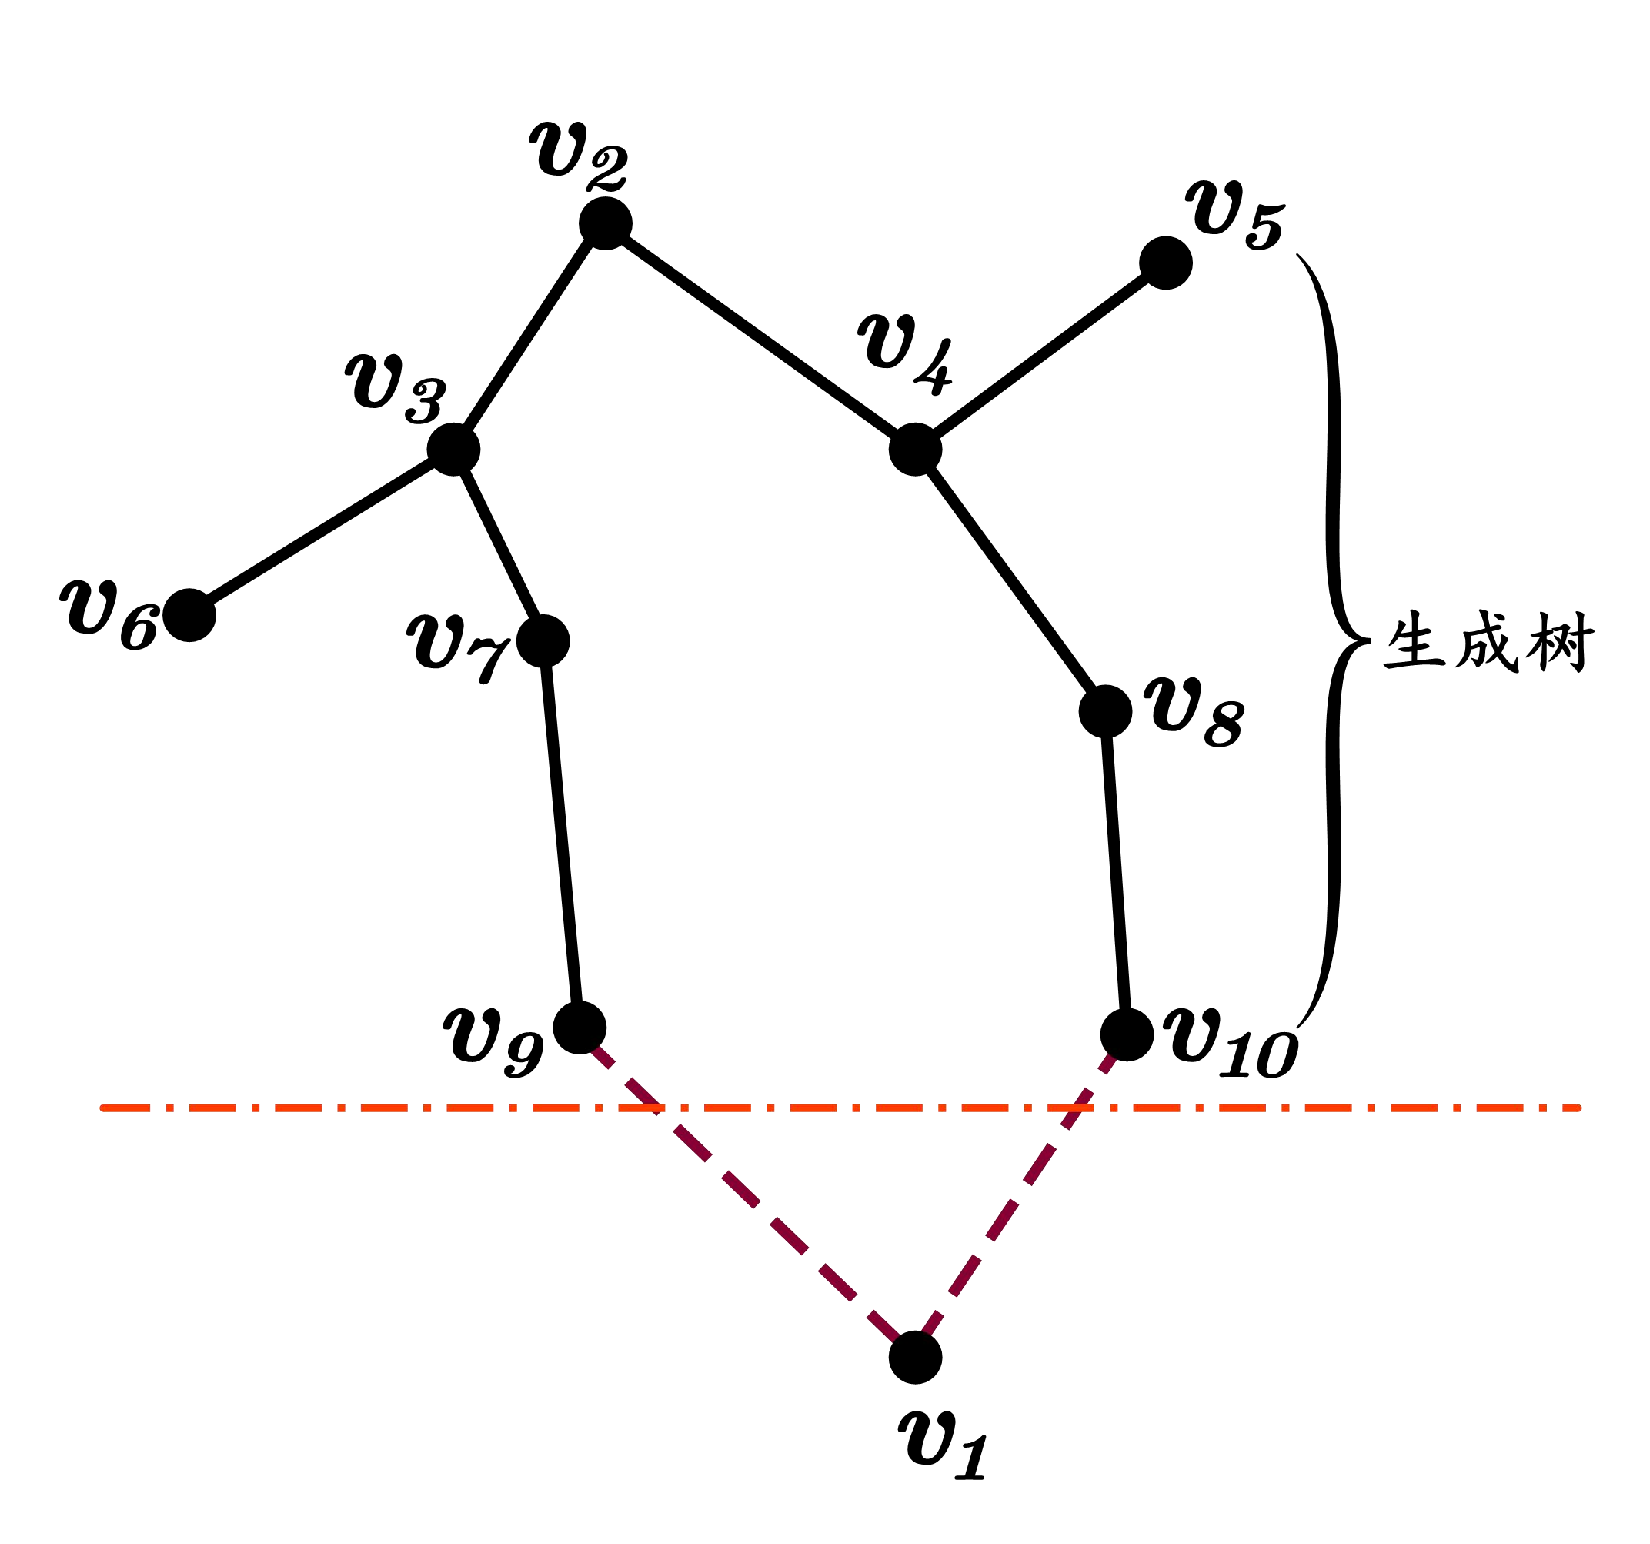
\includegraphics[width=.45\linewidth]{生成1-tree.pdf}
    \caption[生成1-tree示意图]{生成1-tree示意图 \\ 红虚线上方的是一颗不包含点$v_1$的生成树。点$v_1$通过两条边($e_{1,9}, e_{1,10}$)连接到生成树上。其中点$v_1$是任意的。图中生成1-tree包含一个回路$<e_{2,3}, e_{3,7}, e_{7,9}, e_{9,1}, e_{1,10}, e_{10,8}, e_{8,4}, e_{4,2}>$}
    \label{fig:生成1-tree示意图}
\end{figure}
\begin{definition}[最小生成1-tree]
    \label{def:Minimum Spanning 1-tree}
    在无向加权图$\mathcal{G}$中,所有边权和最小的生成1-tree(\autoref{def:Spanning 1-Tree}),称为图$\mathcal{G}$的最小生成1-tree(Minimum Spanning 1-tree,\emph{\textbf{1MST}})。
\end{definition}
\begin{definition}[点度]
    \label{def:Degree}
    顶点的度(\emph{\textbf{Degree}}),即该顶点所连接的边的数量。    
\end{definition}
\par
由哈密顿回路(巡回路径)(\autoref{def:Hamiltonian Cycle}),点度(\autoref{def:Degree})和最小生成1-tree(\autoref{def:Minimum Spanning 1-tree})等定义,可以得到以下推论:
\begin{corollary}
    \label{cor:Optimal Tour1}
    最优巡回路径(\autoref{def:Hamiltonian Cycle})是每个点度(\autoref{def:Degree})为2的最小生成1-tree(\autoref{def:Minimum Spanning 1-tree})。
\end{corollary}
\begin{corollary}
    \label{cor:Optimal Tour2}
    如果一个最小生成1-tree(\autoref{def:Minimum Spanning 1-tree})是巡回路径(\autoref{def:Hamiltonian Cycle}),则该巡回路径是最优的。
\end{corollary}
\par
由上述推论可以知道,TSP问题的最优解就是一个所有点度为2的1MST。但是,1MST一般是不规整的(点度不都为2),即便这样,一个不规整的1MST也会包含大量与最优巡回路径相同的边。而我们构造邻域结构的目的,就是为了在稀疏化图的同时,尽可能的包含这些可能在最优巡回路径中的边。因此,由1MST来构造的邻域结构具有更好的质量。


\subsection{欧拉回路}
\label{subsec:NS_Method:相关定义与基本概念:欧拉回路}
在图论中,欧拉路径(Eulerian Path)是连通图中的一条路径,它只访问图中的边一次(允许重复访问同一个顶点),且访问的起始点和终点不同。当访问的起始点和终点相同时,这条路径即为欧拉回路(Eulerian Cycle)。1736年,Leonhard Euler在解决著名的七桥问题时首次讨论了它们\cite{barnett2005early}。下面,将详细介绍与欧拉回路相关的定义和基本概念。
\begin{definition}[欧拉路径]
    \label{def:Eulerian Path}
    遍历连通图的每条边一次且仅一次,并且有不同的起始点和终点的路径,称为欧拉路径(\emph{\textbf{Eulerian Path}})。
\end{definition}  
\begin{definition}[欧拉回路]
    \label{def:Eulerian Cycle}
    欧拉回路(\emph{\textbf{Eulerian Cycle}})是起始点和终点相同的欧拉路径(\autoref{def:Eulerian Path})。
\end{definition}  
\begin{figure}[htb]
    \subfloat[无向连通图 \label{subfig:无向连通图1}]{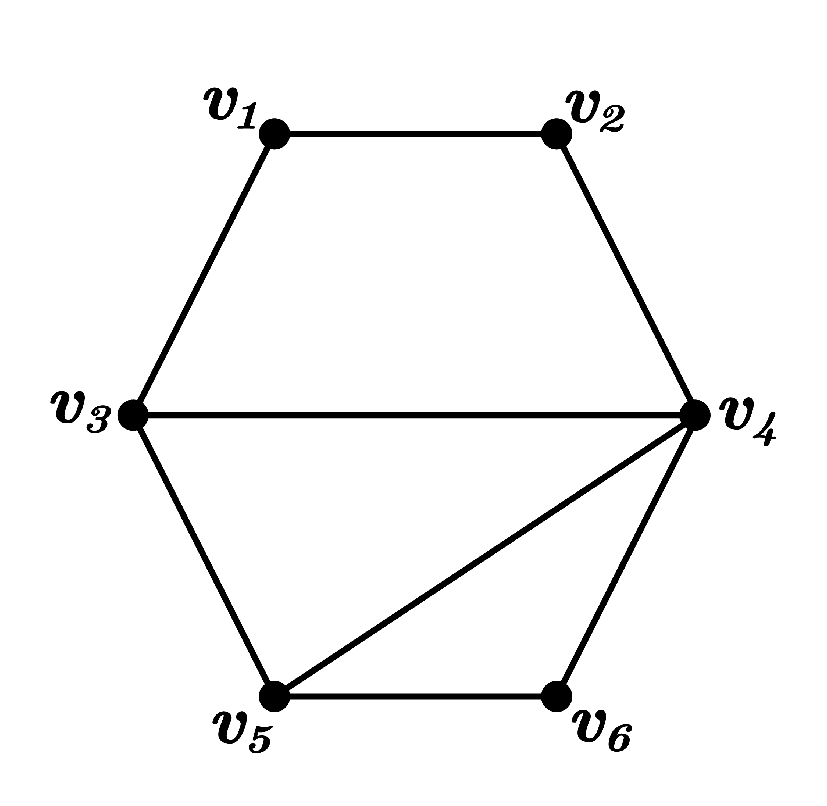
\includegraphics[width=.4\linewidth]{Euler Path Graph.pdf}}\quad
    \subfloat[欧拉路径 \label{subfig:欧拉路径}]{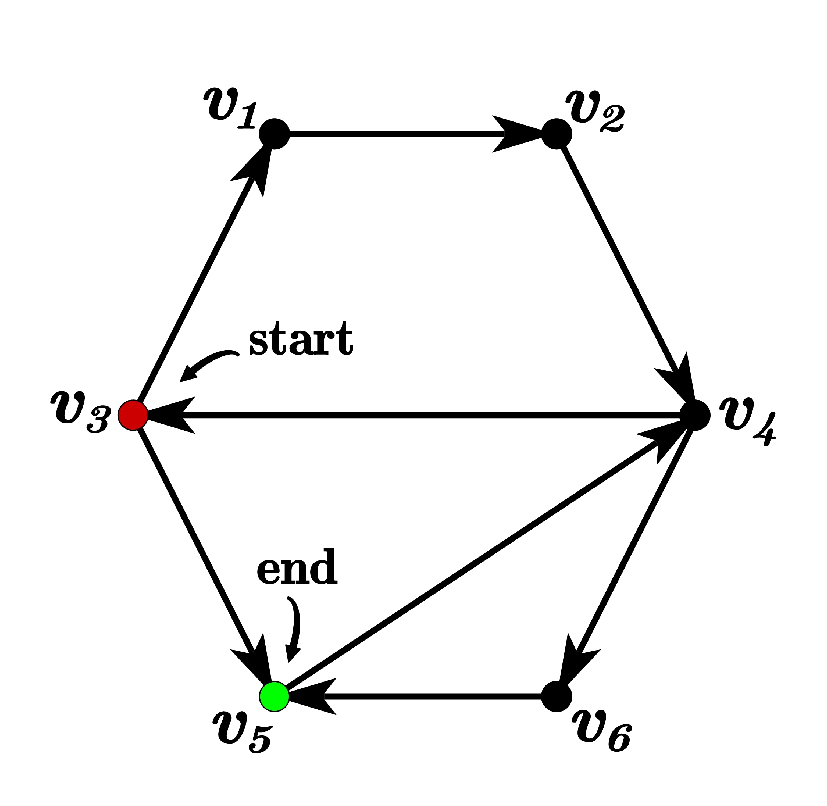
\includegraphics[width=.4\linewidth]{Euler Path.pdf}}
    \caption[欧拉路径示意图]{欧拉路径示意图 \\ 子图\subref{subfig:无向连通图1}~是无向连通图,子图\subref{subfig:欧拉路径}~是子图\subref{subfig:无向连通图1}~的一条欧拉路径$<v_3, v_1, v_2, v_4, v_3, v_5, v_4, v_6, v_5>$}
    \label{fig:欧拉路径示意图}
\end{figure}
\par
如\autoref{fig:欧拉路径示意图}~所示,\autoref{subfig:欧拉路径}~中的欧拉路径是\autoref{subfig:无向连通图1}~中无向连通图的其中一条欧拉路径,这条欧拉路径通过每条边一次,并且在不同的顶点开始($v_3$)和结束($v_5$)。但是,\autoref{subfig:无向连通图1}~中不存在欧拉回路,因为不存在起始点和终点相同的欧拉路径。
\begin{figure}[htb]
    \subfloat[无向连通图 \label{subfig:无向连通图2}]{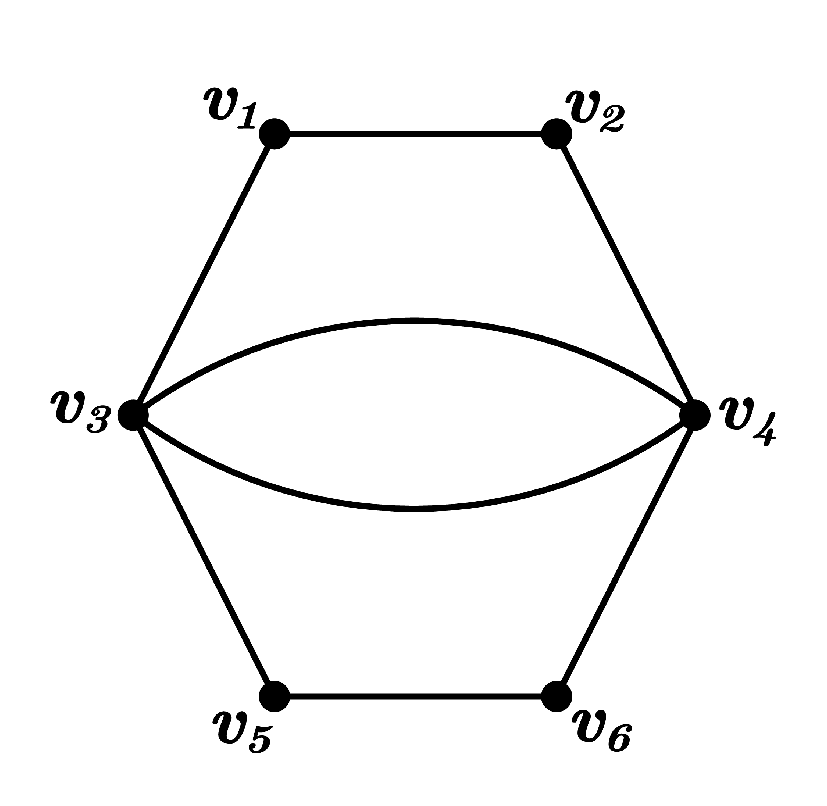
\includegraphics[width=.4\linewidth]{Euler Circuit Graph.pdf}}\quad
    \subfloat[欧拉回路 \label{subfig:欧拉回路}]{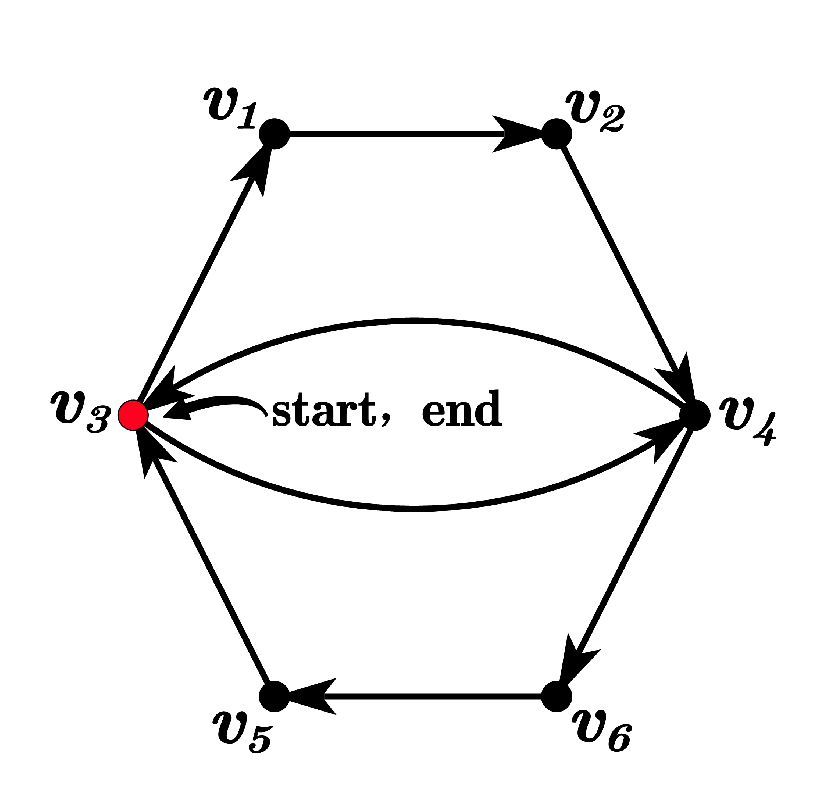
\includegraphics[width=.4\linewidth]{Euler Circuit.pdf}}
    \caption[欧拉回路示意图]{欧拉回路示意图 \\ 子图\subref{subfig:无向连通图2}~是无向连通图,子图\subref{subfig:欧拉回路}~是子图\subref{subfig:无向连通图2}~的一条欧拉回路$<v_3, v_1, v_2, v_4, v_6, v_5, v_3, v_4, v_3>$}
    \label{fig:欧拉回路示意图}
\end{figure}
\par
如\autoref{fig:欧拉回路示意图}~所示,\autoref{subfig:欧拉回路}~中的欧拉回路是\autoref{subfig:无向连通图2}~中无向连通图的其中一条欧拉回路,这条欧拉回路通过每条边一次,并且在同一顶点($v_3$)开始和结束。
\begin{theorem}
    \label{thm:欧拉回路}
    如果一个无向连通图存在度数为奇数的点,则它必定不存在欧拉回路。
\end{theorem}
\begin{corollary}
    \label{cor:欧拉回路}
    如果一个无向连通图的每一个点的度数都为偶数,则它必定存在至少一条欧拉回路。
\end{corollary}
\par
本文需要使用欧拉回路的目的在于将欧拉回路当做1MST和Tour相互转换的一个桥梁。首先,通过将1MST转变为欧拉回路,然后再用欧拉回路来构造Tour。由\autoref{thm:欧拉回路}~和\autoref{cor:欧拉回路}~可以看出,获取欧拉回路的前提是这个图的每个点的度数应该都为偶数。因此,我们需要将1MST改造成每个点都为偶数的图。

\subsection{次梯度优化}
\label{subsec:NS_Method:相关定义与基本概念:次梯度优化}
在章节\ref{subsec:NS_Method:相关定义与基本概念:最小生成1-tree}~中介绍了生成1-tree(\autoref{def:Spanning 1-Tree})和1MST(\autoref{def:Minimum Spanning 1-tree}),而次梯度优化\cite{held1971traveling}是一种可用于优化生成1-tree的方法。从\autoref{cor:Optimal Tour1}~和\autoref{cor:Optimal Tour2}~可知,每一条巡回路径(Tour)都是一颗生成1-tree,所以,1MST的边权和是最优Tour边权和的下界。次梯度优化的作用就是通过对原权重矩阵进行变换,从而不断的优化提高这个下界,用以逼近最优Tour的边权和,这样就能使得最终的邻域结构中包含尽可能多的最优Tour中的边。权重矩阵变换\cite{held1971traveling}可陈述如下:
\begin{itemize}
    \item 如果一个点的所有关联边的权重都以相同的量($\pi$,惩罚值)改变,则原最优Tour不随值$\pi$改变而改变,仍然保持最优。因此,设有权重矩阵$W = (w_{i,j}), \ i,j \in \{ 1, \cdots, n\}$,其中,$w_{i,j}$是边$e_{i,j}$的权重,由此可得转换后的矩阵
    \begin{align}
        \label{eq:Pi权重矩阵}
        W' & = (w'_{i,j}), \\
        w'_{i,j} & = w_{i,j} + \pi_{i} + \pi_{j}, \notag \\
        i,j & \in \{ 1, \cdots, n\}. \notag
    \end{align}
    则可知,$W'$的最优Tour同样也是$W$的最优Tour。由$W'$获取的每条Tour都比$W$所获取的Tour的边权和多$2\sum \pi_i, \ i \in \{1, \cdots, n\}$。使用这种权重矩阵变换,不会改变原问题的最优Tour,但是通常会改变生成的1MST。
    \item 假设$\mathcal{T}_{\pi}$是图$\mathcal{G} = \{ V, E, W' \}$的1MST,$L(\mathcal{T}_{\pi})$为$\mathcal{T}_{\pi}$的边权和,则$L(\mathcal{T}_{\pi})$是$W'$的最优Tour的下界,因此,$\mathcal{L}(\mathcal{T}_{\pi}) = L(\mathcal{T}_{\pi}) - 2\sum \pi_i, \ i \in \{1, \cdots, n\}$是$W$的最优Tour的下界。
\end{itemize}
综上,优化提高最优Tour的边权和的下界的目标就转换成:优化一个变换$W \xrightarrow[]{\mathbf{\pi}} W'$,其中$\mathbf{\pi} = (\pi_1, \cdots, \pi_n)^T$,最大化下界$\mathcal{L}(\mathcal{T}_{\pi}) = L(\mathcal{T}_{\pi}) - 2\sum \pi_i, \ i \in \{1, \cdots, n\}$。由于$\mathcal{L}(\mathcal{T}_{\pi})$是凹的分段线性函数且不可微。因此适合用次梯度(梯度的扩展)优化来最大化$\mathcal{L}(\mathcal{T}_{\pi})$,它是一种通过逐步改变$\pi$来近似$\mathcal{L}(\mathcal{T}_{\pi})$最大值的迭代方法。
\par
\begin{algorithm}[!h]
    \setstretch{1.3}
    \caption{次梯度优化}
    \label{alg:次梯度优化}
    \BlankLine
    \KwIn{ \\
        \hspace{1em} $W$:权重矩阵 \\
        \hspace{1.1em} $n \ $:顶点个数
    }
    \KwOut{$\mathbf{\pi}$}
    \tcp{初始化向量$\pi$,衰减周期$Period$,步长$\sigma$,阶段$Phase$}
    $\mathbf{\pi},\mathbf{\pi^*} \leftarrow \mathbf{0}; \ Period = n/2; \ \sigma = 1; \ Phase = 1 $ \;
    \tcp{使用prim获取$\mathcal{T}$,$L(\mathcal{T})$为$\mathcal{T}$的边权和,$D = (d_i)$为$\mathcal{T}$中每个点的度}
    $\mathcal{T} \xleftarrow[]{prim} W; \ L^* \xleftarrow[]{L(\mathcal{T})} \mathcal{T}; \ D \xleftarrow[]{degree} \mathcal{T}; \ D' \xleftarrow[]{copy} D$ \;
    $Norm(D) = \sum_{i=1}^{n} (d_i-2)^2, \ d_i \in D $ \;
    \lIf(\tcp*[f]{如果Norm为0,说明1MST是Tour}){$Norm(D)==0$}{\textbf{return } $\mathbf{\pi}$}
    \While{$Period > 0 \ $ and $\ \sigma > 0 \ $ and $\ Norm \not = 0$}{
        $P = 1$ \;
        \While{$\sigma > 0\ $ and $\ P \leq Period \ $ and $\ Norm \not = 0$}{
            \For{$i = 1 \ $ to $ \ n$}{
                \lIf{$d_i \not = 2$}{
                    $\pi_i \ += \ \sigma (0.7(d_i-2) + 0.3(d'_i-2))$ \label{line:更新pi}
                }
                $d'_i = d_i$ \;
            }
            $W' \xleftarrow[]{} W + \mathbf{\pi}; \ \mathcal{T} \xleftarrow[]{prim} W'; \ D \xleftarrow[]{degree} \mathcal{T}$ \label{line:1MST} \;
            \lIf{$Norm(D)==0$}{\textbf{return } $\mathbf{\pi^*}$}
            \uIf{$L(\mathcal{T}) > L^*$}{
                $L^* = L(\mathcal{T}); \ \mathbf{\pi^*} = \mathbf{\pi}$ \;
                \lIf{$Phase==1$}{$\sigma \ *= \ 2$}  \label{line:更新步长1}
                \lIf{$Period==P$}{$Period \ *= \ 2$}
            }
            \ElseIf{$Phase==1 \ $ and $\ P > Period/2$}{
                $Period = 0; \ P = 0; \ \sigma *= 3/4 $ \label{line:更新步长2} \;
            }
            $P \ += \ 1$ \;
        }
        $Period \ /= \ 2; \ \sigma \ /= \ 2$ \label{line:更新步长3} \;
    }
    \textbf{return } $\mathbf{\pi^*}$ \;
\end{algorithm}
\par
对于最大化问题$\mathcal{L}(\mathcal{T})$而言,$D$为$\mathcal{T}$中节点的度数向量,可以知道$D-2$为次梯度向量。次梯度优化就是使得$\mathcal{T}$的节点度数往$D=2$的方向优化。算法\ref{alg:次梯度优化}~展示的就是次梯度优化的详细过程。在算法\ref{alg:次梯度优化}~关键步骤在于惩罚值$\mathbf{\pi}$和步长$\sigma$的更新。在第~\ref{line:更新pi}~行中,$\mathbf{\pi}$根据当前1MST和上一迭代时间的1MST的节点度向量按照一定的比重求和,再与当前步长$\sigma$相乘作为当前$\mathbf{\pi}$的更新量,这使得$\mathcal{T_{\pi}}$往最优Tour的方向优化。第(\ref{line:更新步长1},\ref{line:更新步长2},\ref{line:更新步长3})行是步长$\sigma$更新的方式。步长$\sigma$按照不同周期$Period$和阶段$Phase$来更新的。初始周期迭代次数设为$n/2$,每一个周期结束后,周期和步长都会减半。整个算法过程中,$\sigma$分为两个阶段更新,第一个阶段是$\sigma \ *= \ 2$,第二个阶段是$\sigma \ *= \ 3/4$,这保证了$\mathbf{\pi}$在前期能够大幅度的更新,后期能够控制其精细度,使得算法能够快速收敛到理想解\cite{crowder1974computational,hansen1974improvements}。并且从算法流程中可以看出,第~\ref{line:更新步长2}~行中使用不同的$W'$生成了大量未使用的1MST,这正是本文提出的算法所需的。
\par
\begin{figure}[htb]
    \subfloat[初始$\mathcal{T}$ \label{subfig:初始1MST}]{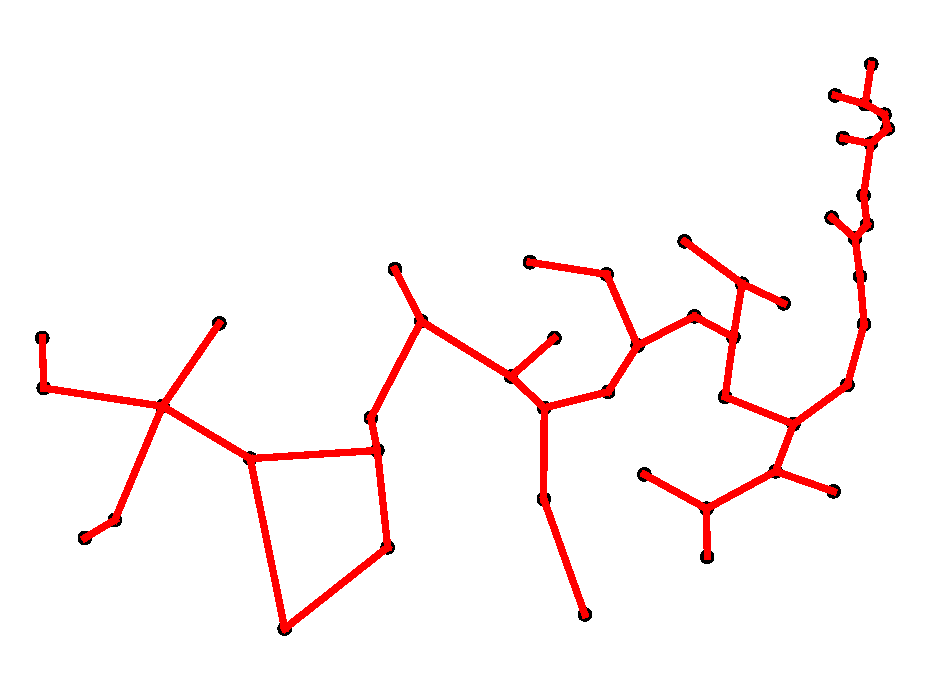
\includegraphics[width=.33\linewidth]{1MST Init.pdf}}
    \subfloat[优化$\mathcal{T_{\pi}}$ \label{subfig:优化1MST}]{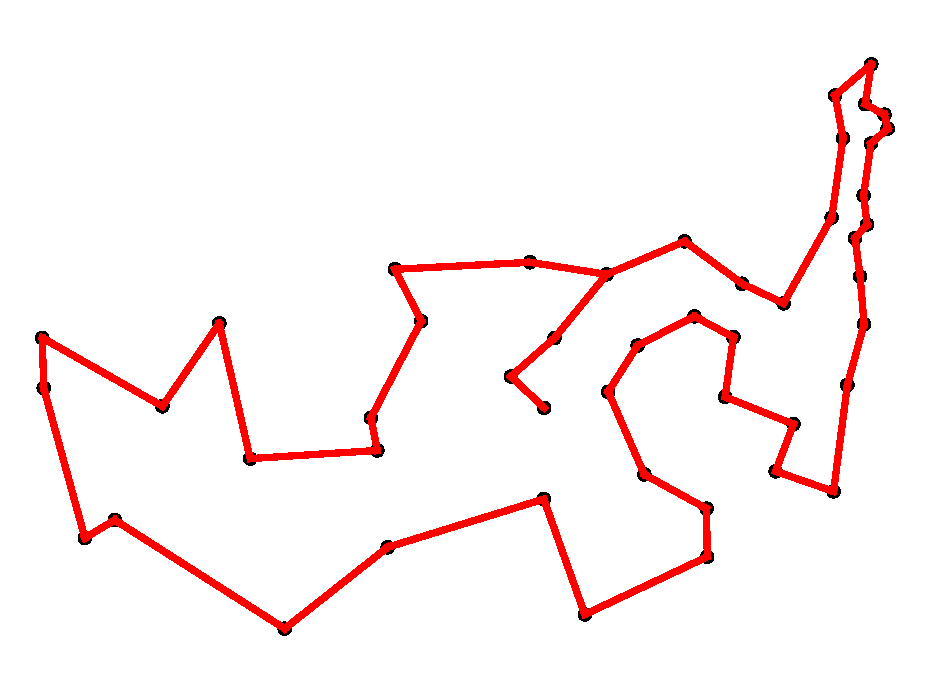
\includegraphics[width=.33\linewidth]{1MST Improved.pdf}}
    \subfloat[最优Tour \label{subfig:最优Tour}]{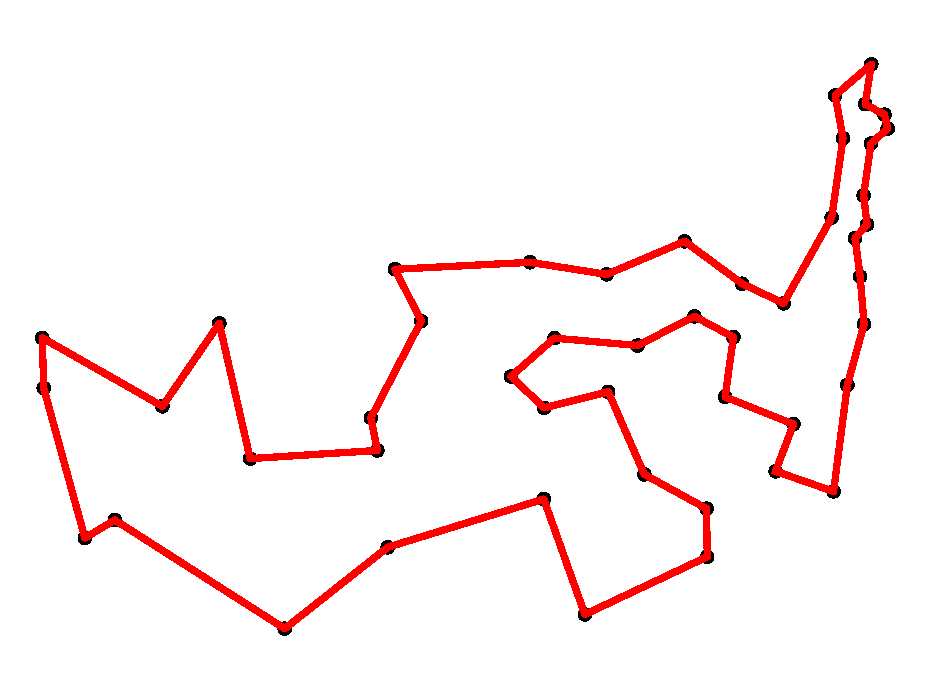
\includegraphics[width=.33\linewidth]{1MST Tour.pdf}}
    \caption[次梯度优化结果示意图]{次梯度优化结果示意图}
    \label{fig:次梯度优化结果示意图}
\end{figure}
\par
\autoref{fig:次梯度优化结果示意图}~中展示了1MST使用次梯度优化后的效果。\autoref{subfig:初始1MST}~是使用原始$W$获取的1MST,\autoref{subfig:优化1MST}~是原始$W$经过次梯度优化后获取的1MST,\autoref{subfig:最优Tour}~展示的是该问题的最优Tour。从图中可以看出,原始1MST经过次梯度优化后,节点的度数都趋向于2,并且包含了大量的最优Tour中的边。

\section{邻域结构生成算法}
\label{sec:NS_Method:邻域结构生成算法}
在这一节,首先将介绍基于最小生成树和欧拉回路的邻域结构(Neighborhood Structure based on Minimum spanning tree and Euler circuit,meNS)生成算法的主框架,然后会分节介绍算法中各个子部分。包括使用1MST来构造Tour以及使用循环扫描局部优化来对Tour进行初步的优化。

\subsection{meNS生成算法主框架}
\label{subsec:NS_Method:邻域结构生成算法:meNS主框架}
实现meNS生成算法的关键在于如何高效的生成一系列中等质量的初始Tour,因为这些初始Tour中必定包含大量的最优Tour中的边。算法利用这一系列中等质量的Tour,将其拆分并重新组装构造成一个完整的邻域结构。从算法\ref{alg:次梯度优化}~可以知道,算法产生了大量的未被使用的1MST。而meNS生成算法的核心思想就是利用这些未被使用的1MST,用欧拉回路最为桥梁,将其转变为Tour。经过1MST转变来的Tour的质量会比随机生成的好很多,因此,这个步骤将节省大部分的优化时间。最后,只需要将这些Tour经过局部优化,就可以得到一个高质量的邻域结构。meNS生成算法主框架如下:
\par
\begin{algorithm}
    \setstretch{1.3}
    \caption{meNS生成算法主框架}
    \label{alg:meNS生成算法主框架}
    \BlankLine
    \KwIn{ \\
        \hspace{1.1em} $T \ $:$\{ \mathcal{T}_1, \cdots, \mathcal{T}_k \}$ \\
        \hspace{1em} $M$:最大候选边数 \\
        \hspace{1.1em} $L \ $:子路径长度 \\
        \hspace{1.1em} $S \ $:扫描次数
    }
    \KwOut{$meNS$}
    $meNS \leftarrow \varnothing$ \label{line:meNS初始化} \;
    \ForEach{$\mathcal{T} \in T$ \label{line:处理1MST}}{
        \tcp{通过$Transform$操作,将$\mathcal{T}$转变为$Tour$}
        $Tour \xleftarrow[]{Transform} \mathcal{T}$ \label{line:1MST转换} \;
        \tcp{通过循环扫描局部优化,对$Tour$进行优化得到$Tour'$}
        $Tour' \xleftarrow[]{Optimize} Tour, L, S$ \label{line:Tour局部优化} \;
        $meNS \leftarrow meNS \bigcup Tour'$ \label{line:并入meNS} \;
    } \label{line:处理1MST结束}
    \tcp{修剪meNS,使得每个点的候选边不超过M条}
    $meNS \xleftarrow[]{Trim} meNS, M$ \label{line:修剪meNS} \;
    \textbf{return } $meNS$ \;
\end{algorithm}
\par
算法\ref{alg:meNS生成算法主框架}~所示为meNS生成算法的主要步骤。第~\ref{line:meNS初始化}~是将邻域结构meNS初始化为空集。第~\ref{line:处理1MST}-\ref{line:处理1MST结束}~行循环处理1MST,将所有的1MST转变为Tour并将其优化。其中,第~\ref{line:1MST转换}~行是将1MST转变为Tour。第~\ref{line:Tour局部优化}~行是对转变得到的Tour进行循环扫描局部优化,得到优化后的$Tour'$。第~\ref{line:并入meNS}~行是将$Tour'$的边并入到邻域结构meNS中。最后,第~\ref{line:修剪meNS}~行是对meNS进行修剪,尽可能的使邻域结构稀疏化。

\subsection{1MST变换}
\label{subsec:NS_Method:邻域结构生成算法:1MST变换}
在算法\ref{alg:meNS生成算法主框架}~中,第~\ref{line:1MST转换}~行使用$Transform$将1MST转换成Tour。在将1MST转换成Tour的过程中,需要先把1MST构造成欧拉回路(\autoref{def:Eulerian Cycle})。根据\autoref{thm:欧拉回路}~和\autoref{cor:欧拉回路}~可知,首先需要将1MST构造成每个点都为偶数度的连通图(欧拉图)。由\autoref{def:Tree}~,\autoref{def:Spanning 1-Tree}~和\autoref{def:Spanning 1-Tree}可知,1MST是具有偶数个(或0个)奇数度节点的连通图,因此,我们只需要将1MST所有的奇数度节点构造成偶数度节点,即可得到欧拉图。一个巧妙的构造方法是将这些奇数度节点根据节点之间的距离分成不同的组,每个组中有两个奇数度节点,然后将每组中的顶点用边链接起来,这样两个奇数度节点就变成了偶数度节点了。其构造过程如算法\ref{alg:Transform}~第~\ref{line:构造成欧拉图}-\ref{line:构造成欧拉图结束}~行所示,其中第\ref{line:closest node}~行就是在$V_{odd}$中获取最近的两个奇度点$v_i, v_j$,第\ref{line:并边}~行将$v_i, v_j$链接成边$e_{i,j}$并入到$G_{euler}$中,最后第\ref{line:删点}~行从$V_{odd}$中删除$v_i, v_j$,最终获得的$G_{euler}$就是欧拉图了。
\par
\begin{algorithm}[htb]
    \setstretch{1.3}
    \caption{Transform}
    \label{alg:Transform}
    \BlankLine
    \KwIn{ \\
        \hspace{1em} $\mathcal{T} = (V, E) \ $:$1MST$
    }
    \KwOut{$Tour$}
    \tcp{初始化欧拉图$G_{euler}$和奇数度点集$V_{odd}$}
    $G_{euler} \xleftarrow[]{\{ e_{i,j} \ | \ e_{i,j} \in E \}} \mathcal{T} $ \label{line:init}\;
    $V_{odd} \xleftarrow[]{} \varnothing $ \;
    \ForEach{$v \in V$}{
        \lIf{$v$ is odd degree}{
            $V_{odd} \leftarrow V_{odd} \bigcup v$
        }
    } \label{line:init end}
    \tcp{将1MST构造成欧拉图}
    \While{$V_{odd} \not = \varnothing$ \label{line:构造成欧拉图}}{
        $v_i, v_j = argmin(\{ d(v_i, v_j) \ | \ v_i, v_j \in V_{odd}, i \not = j \}) $ \label{line:closest node} \;
        $G_{euler} \leftarrow G_{euler} \bigcup (e_{i, j} = (v_i, v_j)) $ \label{line:并边} \;
        $V_{odd} \leftarrow V_{odd}/\{v_i, v_j\}$ \label{line:删点} \;
    } \label{line:构造成欧拉图结束}
    \tcp{从欧拉图中通过\autoref{eq:从欧拉图中获取欧拉回路}~获取欧拉回路}
    $C_{euler} \xleftarrow[]{\text{式}\eqref{eq:从欧拉图中获取欧拉回路}} G_{euler}$ \label{line:从欧拉图中获取欧拉回路} \;
    \tcp{将欧拉回路通过\autoref{eq:将欧拉回路构造成Tour}~构造成Tour}
    $Tour \xleftarrow[]{\text{式}\eqref{eq:将欧拉回路构造成Tour}} C_{euler}$ \label{line:将欧拉回路构造成Tour} \;
    \textbf{return } $Tour$ \;
\end{algorithm}
\par
在算法\ref{alg:Transform}~中,第~\ref{line:init}-\ref{line:init end}~行是初始化阶段,主要作用就是初始化欧拉图和奇数度点集,将1MST中的边并入到初始欧拉图中,并将奇数度点加入到奇数度点集中。第~\ref{line:构造成欧拉图}-\ref{line:构造成欧拉图结束}~行主要是将1MST构造成欧拉图的流程。第\ref{line:从欧拉图中获取欧拉回路}~行通过\autoref{eq:从欧拉图中获取欧拉回路}~从欧拉图中获取欧拉回路:
\vspace{-.5em}
\begin{align}
    \label{eq:从欧拉图中获取欧拉回路}
    C_{euler} = <v_i, v_j, v_k, \cdots, v_m, v_n, v_i>, \\
    \{e_{i,j}, e_{j,k}, \cdots, e_{m,n}, e_{n,i}\} = G_{euler}, \notag \\ 
    e_{i,j} = (v_i, v_j) \in G_{euler}, \ i \not = j. \notag 
\end{align}
\vspace{-.5em}
其中,欧拉回路$C_{euler}$中路径序列所组成的边就是欧拉图$G_{euler}$中的所有边,且这些边不重复,但是点可以重复使用。在第\ref{line:将欧拉回路构造成Tour}~行通过\autoref{eq:将欧拉回路构造成Tour}~将欧拉回路构造成Tour:
\vspace{-.5em}
\begin{align}
    \label{eq:将欧拉回路构造成Tour}
    Tour = <v_i, v_j, \cdots, v_n, v_i>, \\ 
    v_i, \cdots, v_n \in C_{euler}, \ i \not = n. \notag
\end{align}
其中,Tour是按照欧拉回路$C_{euler}$中路径序列的顺序,去除重复的点所构成的一个路径序列。可以知道Tour也包含了欧拉图中的所有点,除去首尾节点相同,其他节点都不相同。
\par
\autoref{fig:1MST构造Tour示意图}~所示是一个1MST转换为Tour的具体实例。其中\autoref{subfig:1MST}~展示的是1MST,它包含了四个奇数度节点$V_{odd} = \{v_3,v_4,v_5,v_6\}$,根据算法\ref{alg:Transform}~第~\ref{line:构造成欧拉图}-\ref{line:构造成欧拉图结束}~行,可以将$V_{odd} = \{v_3,v_4,v_5,v_6\}$中的四个点分成$\{v_3,v_6\}$和$\{v_4,v_5\}$两组,然后将两组中的点分别链接起来得到两条边$e_{3,6} = (v_3,v_6)$和$e_{4,5} = (v_4,v_5)$,然后将$e_{3,6}$和$e_{4,5}$并入到$G_{euler}$中,最终获取到的$G_{euler}$为欧拉图,如\autoref{subfig:欧拉图}~所示,其中红色的边即为$e_{3,6}$和$e_{4,5}$。然后遍历欧拉图$G_{euler}$中的边,根据\autoref{eq:从欧拉图中获取欧拉回路}~可以得到一条欧拉回路$C_{euler} = <v_1, v_9, v_7, v_3, v_6, v_3, v_2, v_4, v_5, v_4, v_8, v_{10}, v_1>$,最后根据\autoref{eq:将欧拉回路构造成Tour}~,删除欧拉回路$C_{euler}$中重复的点,可以得到其中一条$Tour = <v_1, v_9, v_7, v_3, v_6, v_2, v_4, v_5, v_8, v_{10}, v_1>$,如\autoref{subfig:Tour}~所示。
\par
\begin{figure}[htb]
    \subfloat[最小生成1-tree \label{subfig:1MST}]{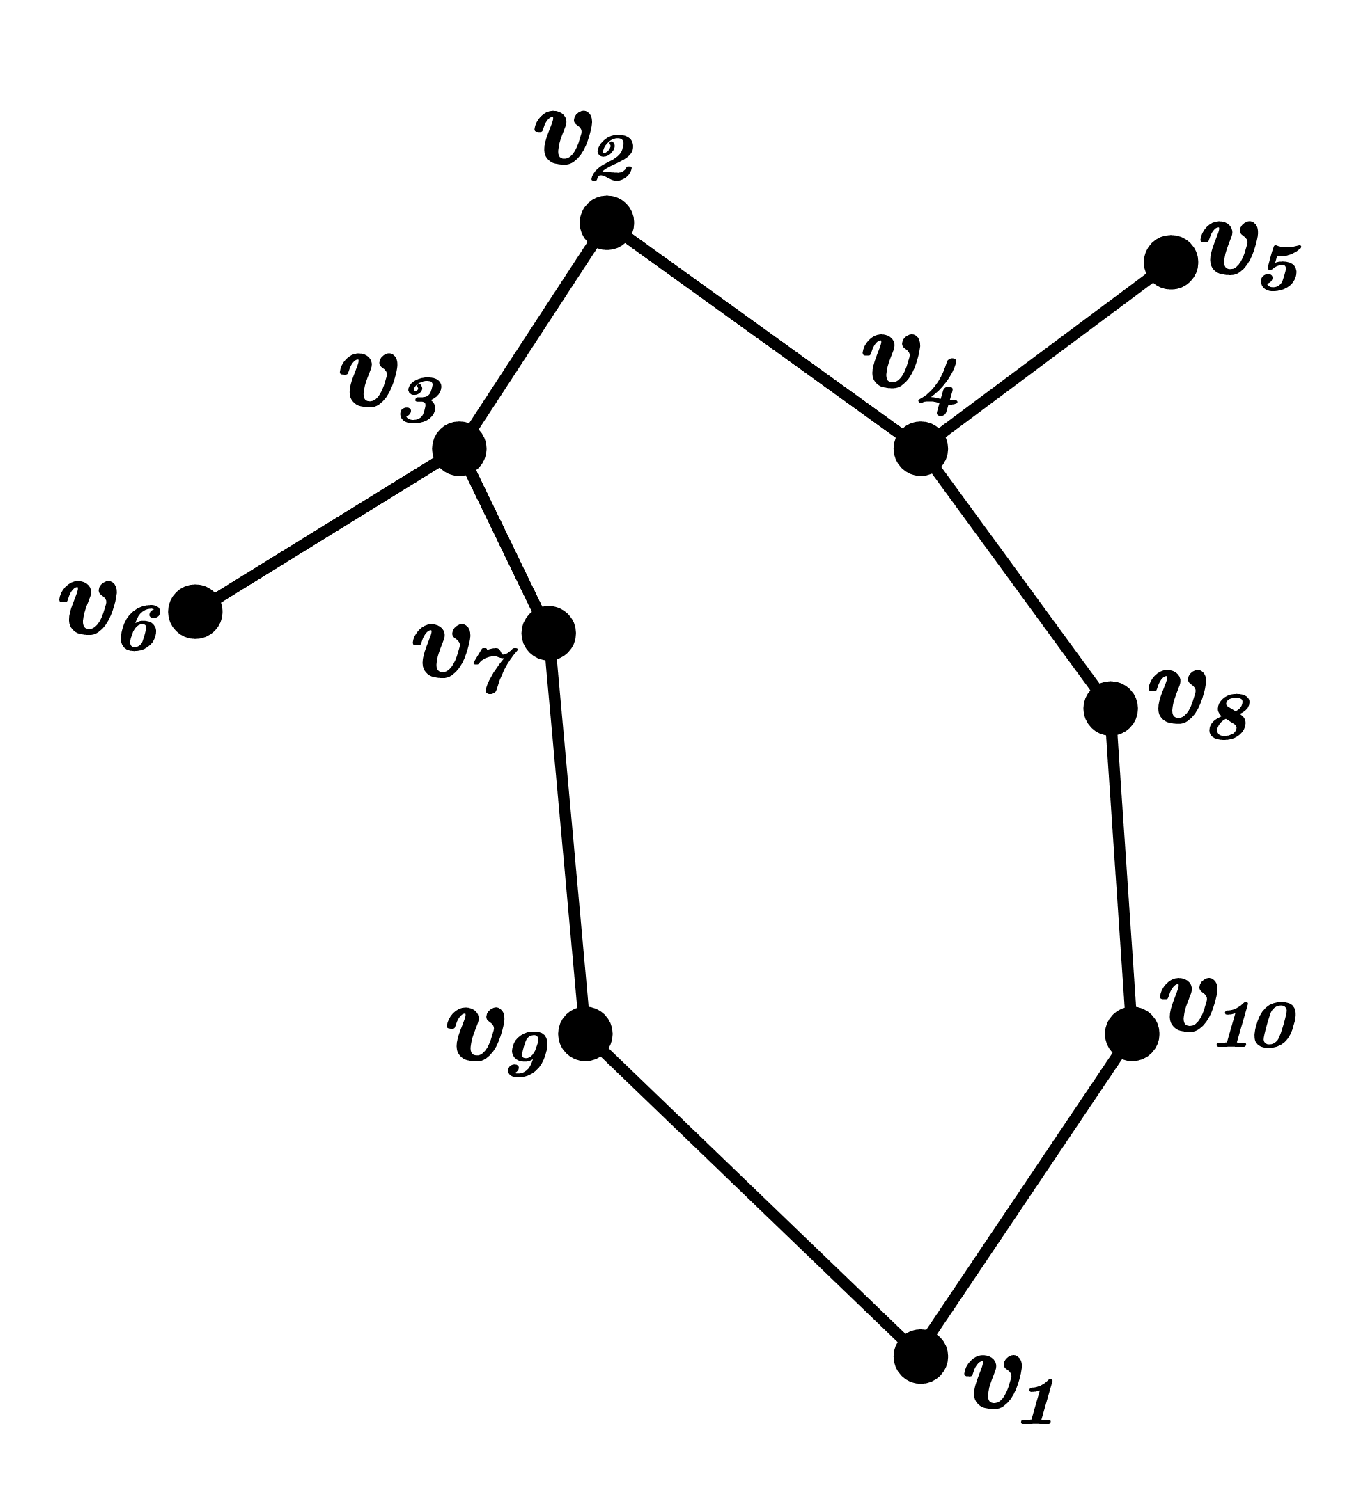
\includegraphics[width=.33\linewidth]{Transform-1MST.pdf}}
    \subfloat[欧拉图 \label{subfig:欧拉图}]{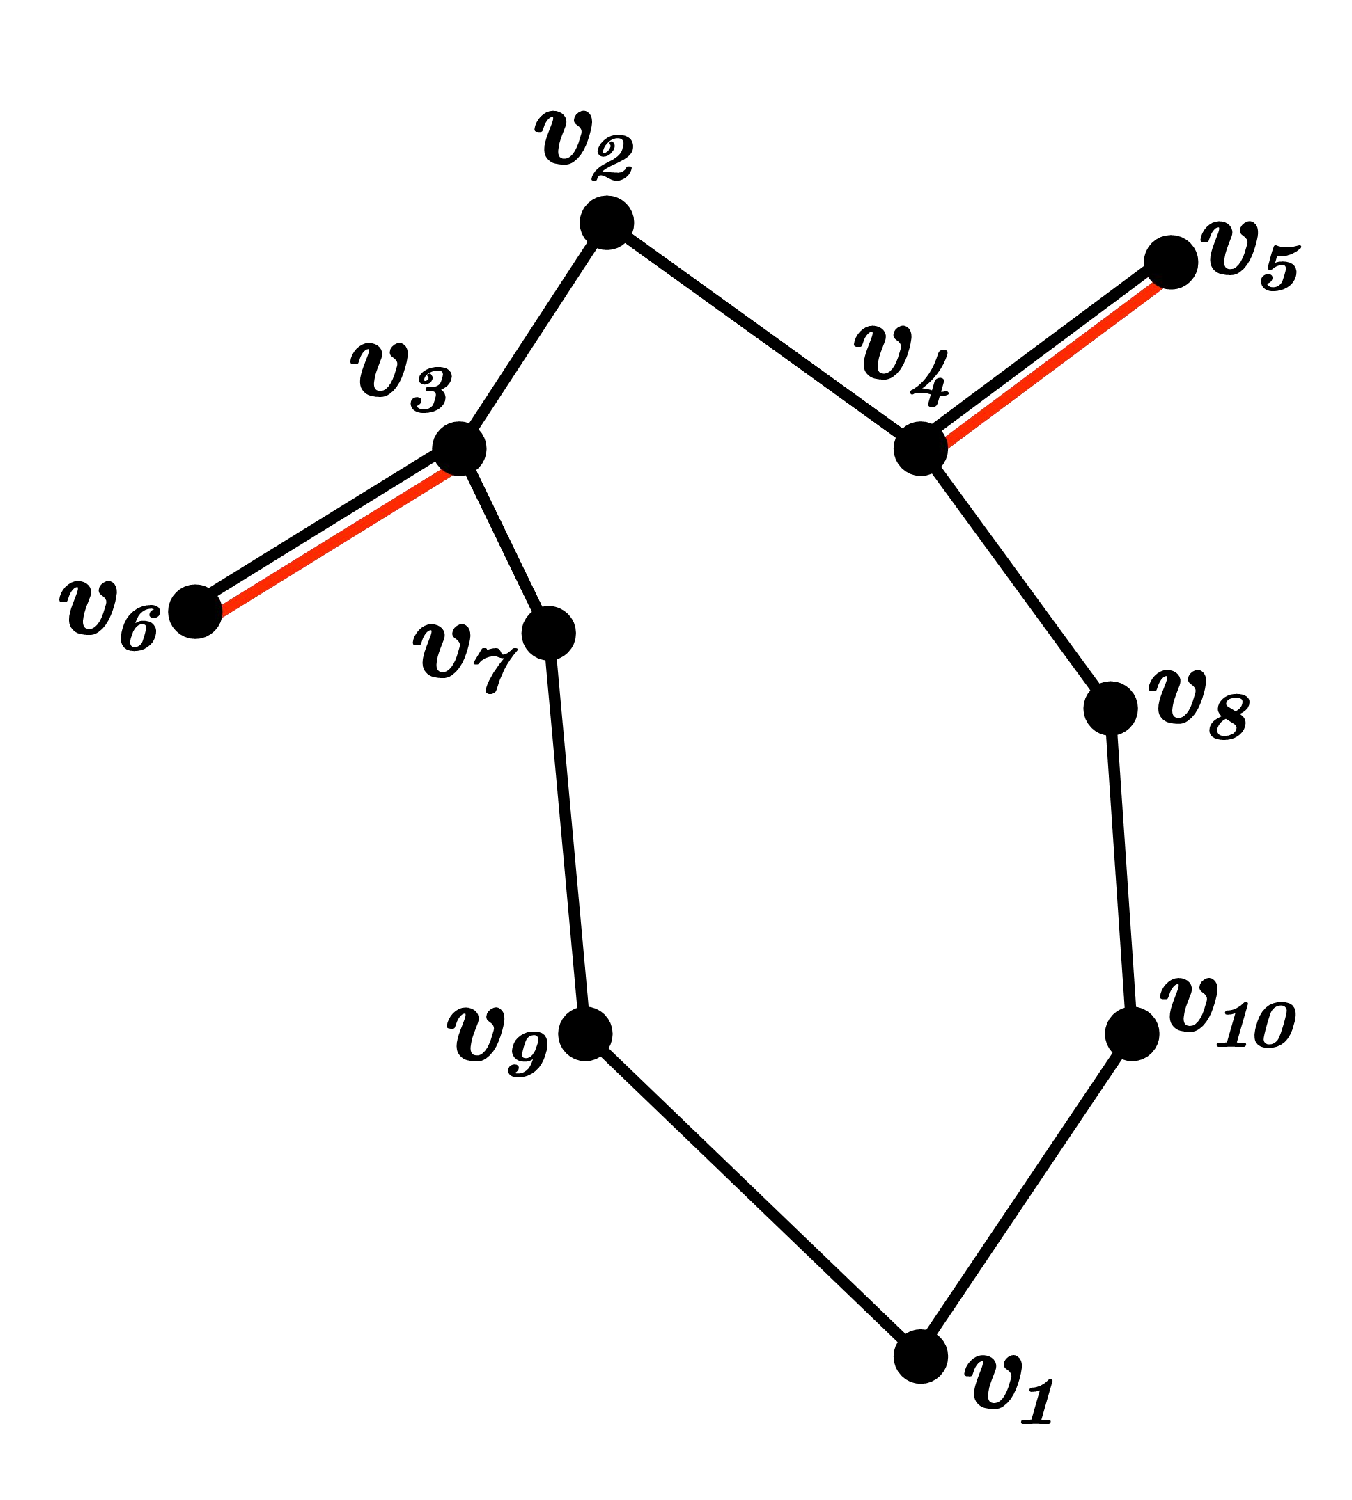
\includegraphics[width=.33\linewidth]{Transform-Euler Graph.pdf}}
    \subfloat[Tour \label{subfig:Tour}]{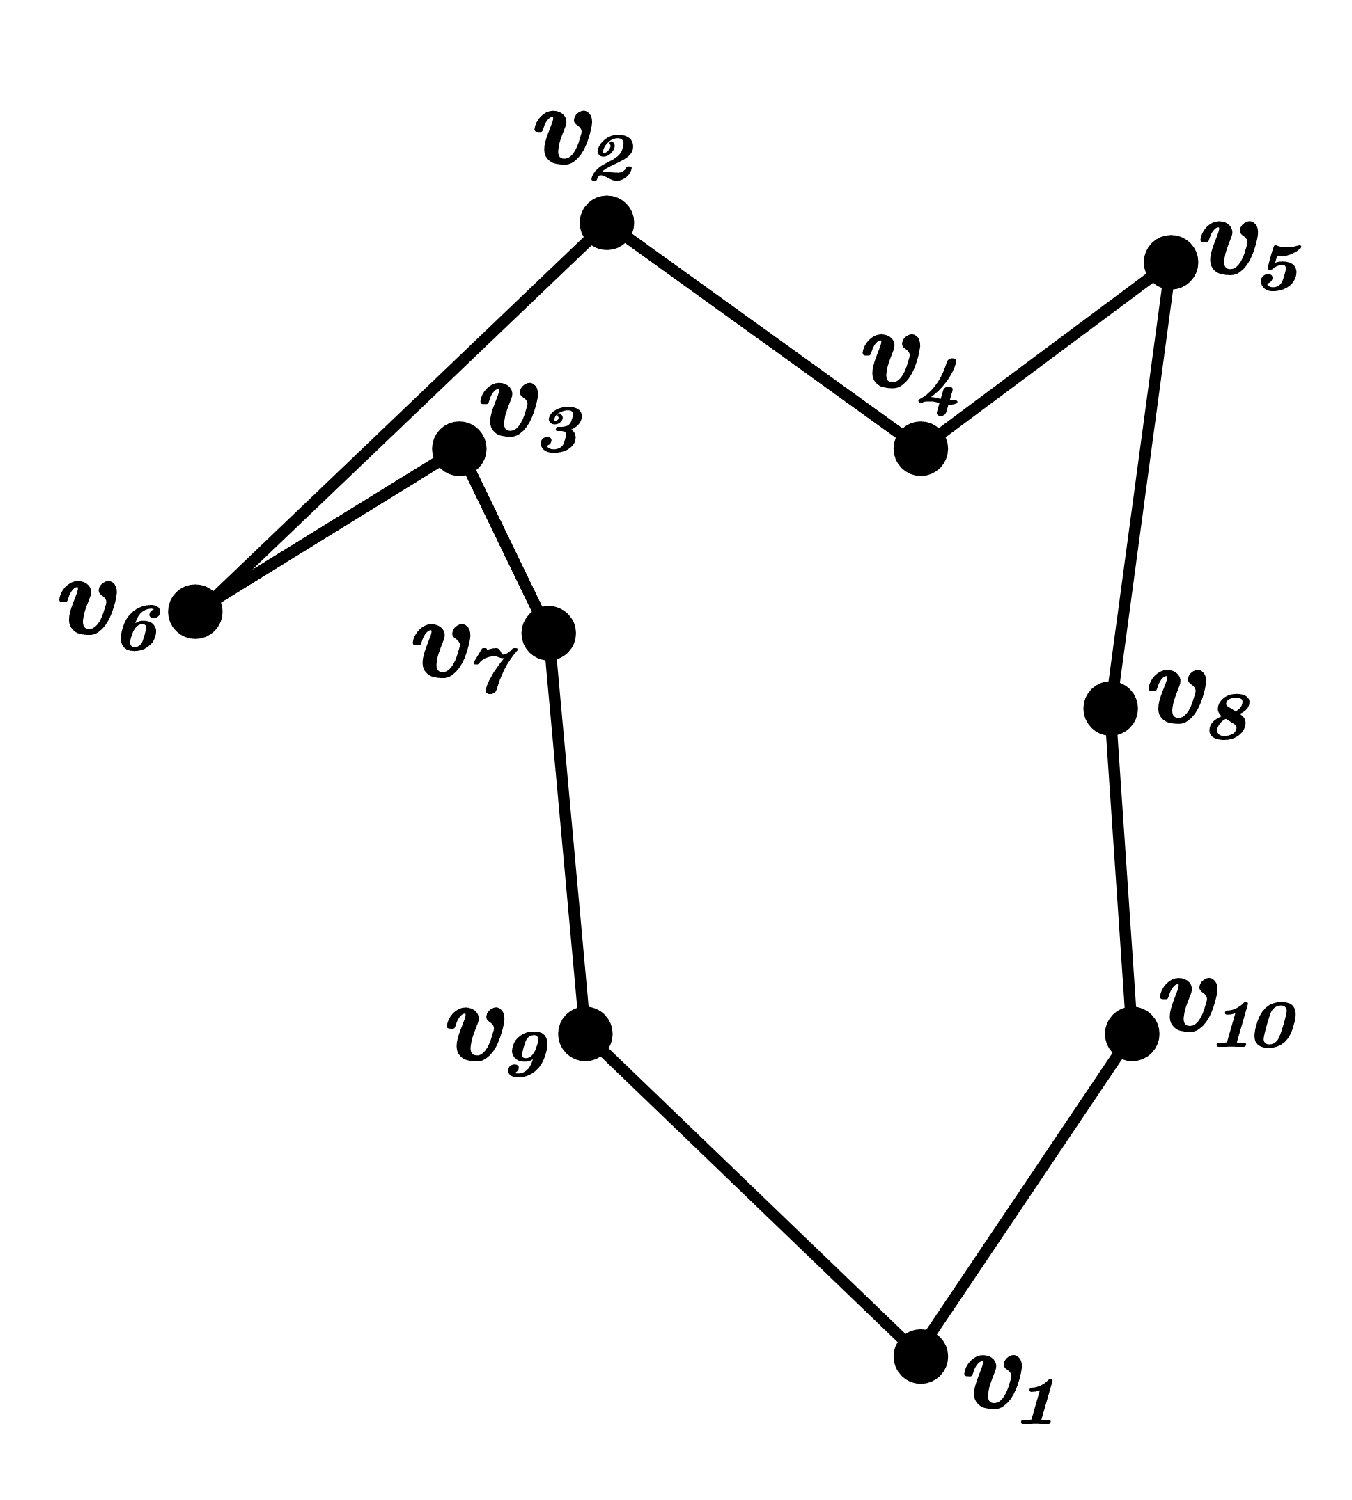
\includegraphics[width=.33\linewidth]{Transform-Tour.pdf}}
    \caption[1MST构造Tour示意图]{1MST构造Tour示意图}
    \label{fig:1MST构造Tour示意图}
\end{figure}

\subsection{循环扫描局部优化}
\label{subsec:NS_Method:邻域结构生成算法:循环扫描局部优化}
在章节\ref{subsec:NS_Method:邻域结构生成算法:1MST变换}~中,算法\ref{alg:Transform}~将1MST构造成了一系列的Tour,本节将介绍一种局部优化的方法,对这些Tour进行更进一步的优化,使得这些Tour尽可能的贴近最优Tour,从而包含更多的最优Tour中的边,以致最终获得的邻域结构的质量更好。其算法流程如下:在算法的输入参数中,$Tour$为待优化的巡回路径;$L$为子路径的长度,因为在算法中,局部优化是以$L$长度为单位进行的,这样就把整个$Tour$分成了$n/L$份,然后对每一个长为$L$的子路径进行局部优化;$S$为算法整体的扫描次数,因为每次扫描后,对整个$Tour$只做了局部的优化,然后对$Tour$通过循环右移的操作将之前的局部性重置,接着再次优化,最后通过多次这样的扫描,使得$Tour$整体都得到优化。
\begin{algorithm}[htb]
    \setstretch{1.3}
    \caption{循环扫描局部优化}
    \label{alg:循环扫描局部优化}
    \BlankLine
    \KwIn{ \\
        \hspace{1.1em} $Tour \ $:待优化Tour \\
        \hspace{1.1em} $L \ $:子路径长度 \\
        \hspace{1.1em} $S \ $:扫描次数
    }
    \KwOut{$Tour \ $:优化后Tour}
    \tcp{Comment}
    $n = |Tour|$ \label{line:节点数} \;
    \For{$i = 1 \ $ to $\ S$ \label{line:扫描}}{
        \lIf{$i \not = 1$}{
            $Tour \xleftarrow[]{\text{循环右移}} Tour, L, S$ \label{line:循环右移}
        }
        \For{$j =0 \ $ to $\ \lfloor n/L \rfloor - 1 $}{
            $Tour \xleftarrow[]{2-opt} Tour, L, jL$ \label{line:局部优化1} \;
        }
        \lIf{$n \% L \not = 0$}{
            $Tour \xleftarrow[]{2-opt} Tour, L, n-L$ \label{line:局部优化2} 
        }
    }\label{line:扫描结束}
    \textbf{return } $Tour$ \;
\end{algorithm}
\par
如算法\ref{alg:循环扫描局部优化}~所示,第~\ref{line:节点数}~行中$|\cdot|$表示集合中元素的个数。第~\ref{line:扫描}-\ref{line:扫描结束}~行是$S$次扫描优化的过程。其中第~\ref{line:循环右移}~是对$Tour$进行整体循环右移$L/S$位,这样可以打破原有的局部性,使得$Tour$能够在全局上得到优化。第~\ref{line:局部优化1}~行和第~\ref{line:局部优化2}~是分别对前$\lfloor n/L \rfloor - 1$个子路径和最后一个子路径进行优化,其中,用到的局部优化算子为2-opt(如\autoref{subfig:2-opt}),因为2-opt的低复杂度能够使子路径快速被优化。循环扫描局部优化如\autoref{fig:循环扫描局部优化示意图}~所示,每次只优化长度为$L$的子路径,再进行了整体的局部优化后,将$Tour$整体向右循环移动$L/S$个位置,经过$S$遍循环扫描后,$Tour$就整体右移了$L$个位置,刚好是一个子路径的长度,这样使得原来优化的局部性通过循环右移的操作扩散到全局,从而使得$Tour$得到了全局性的优化。
\begin{figure}[!htb]
    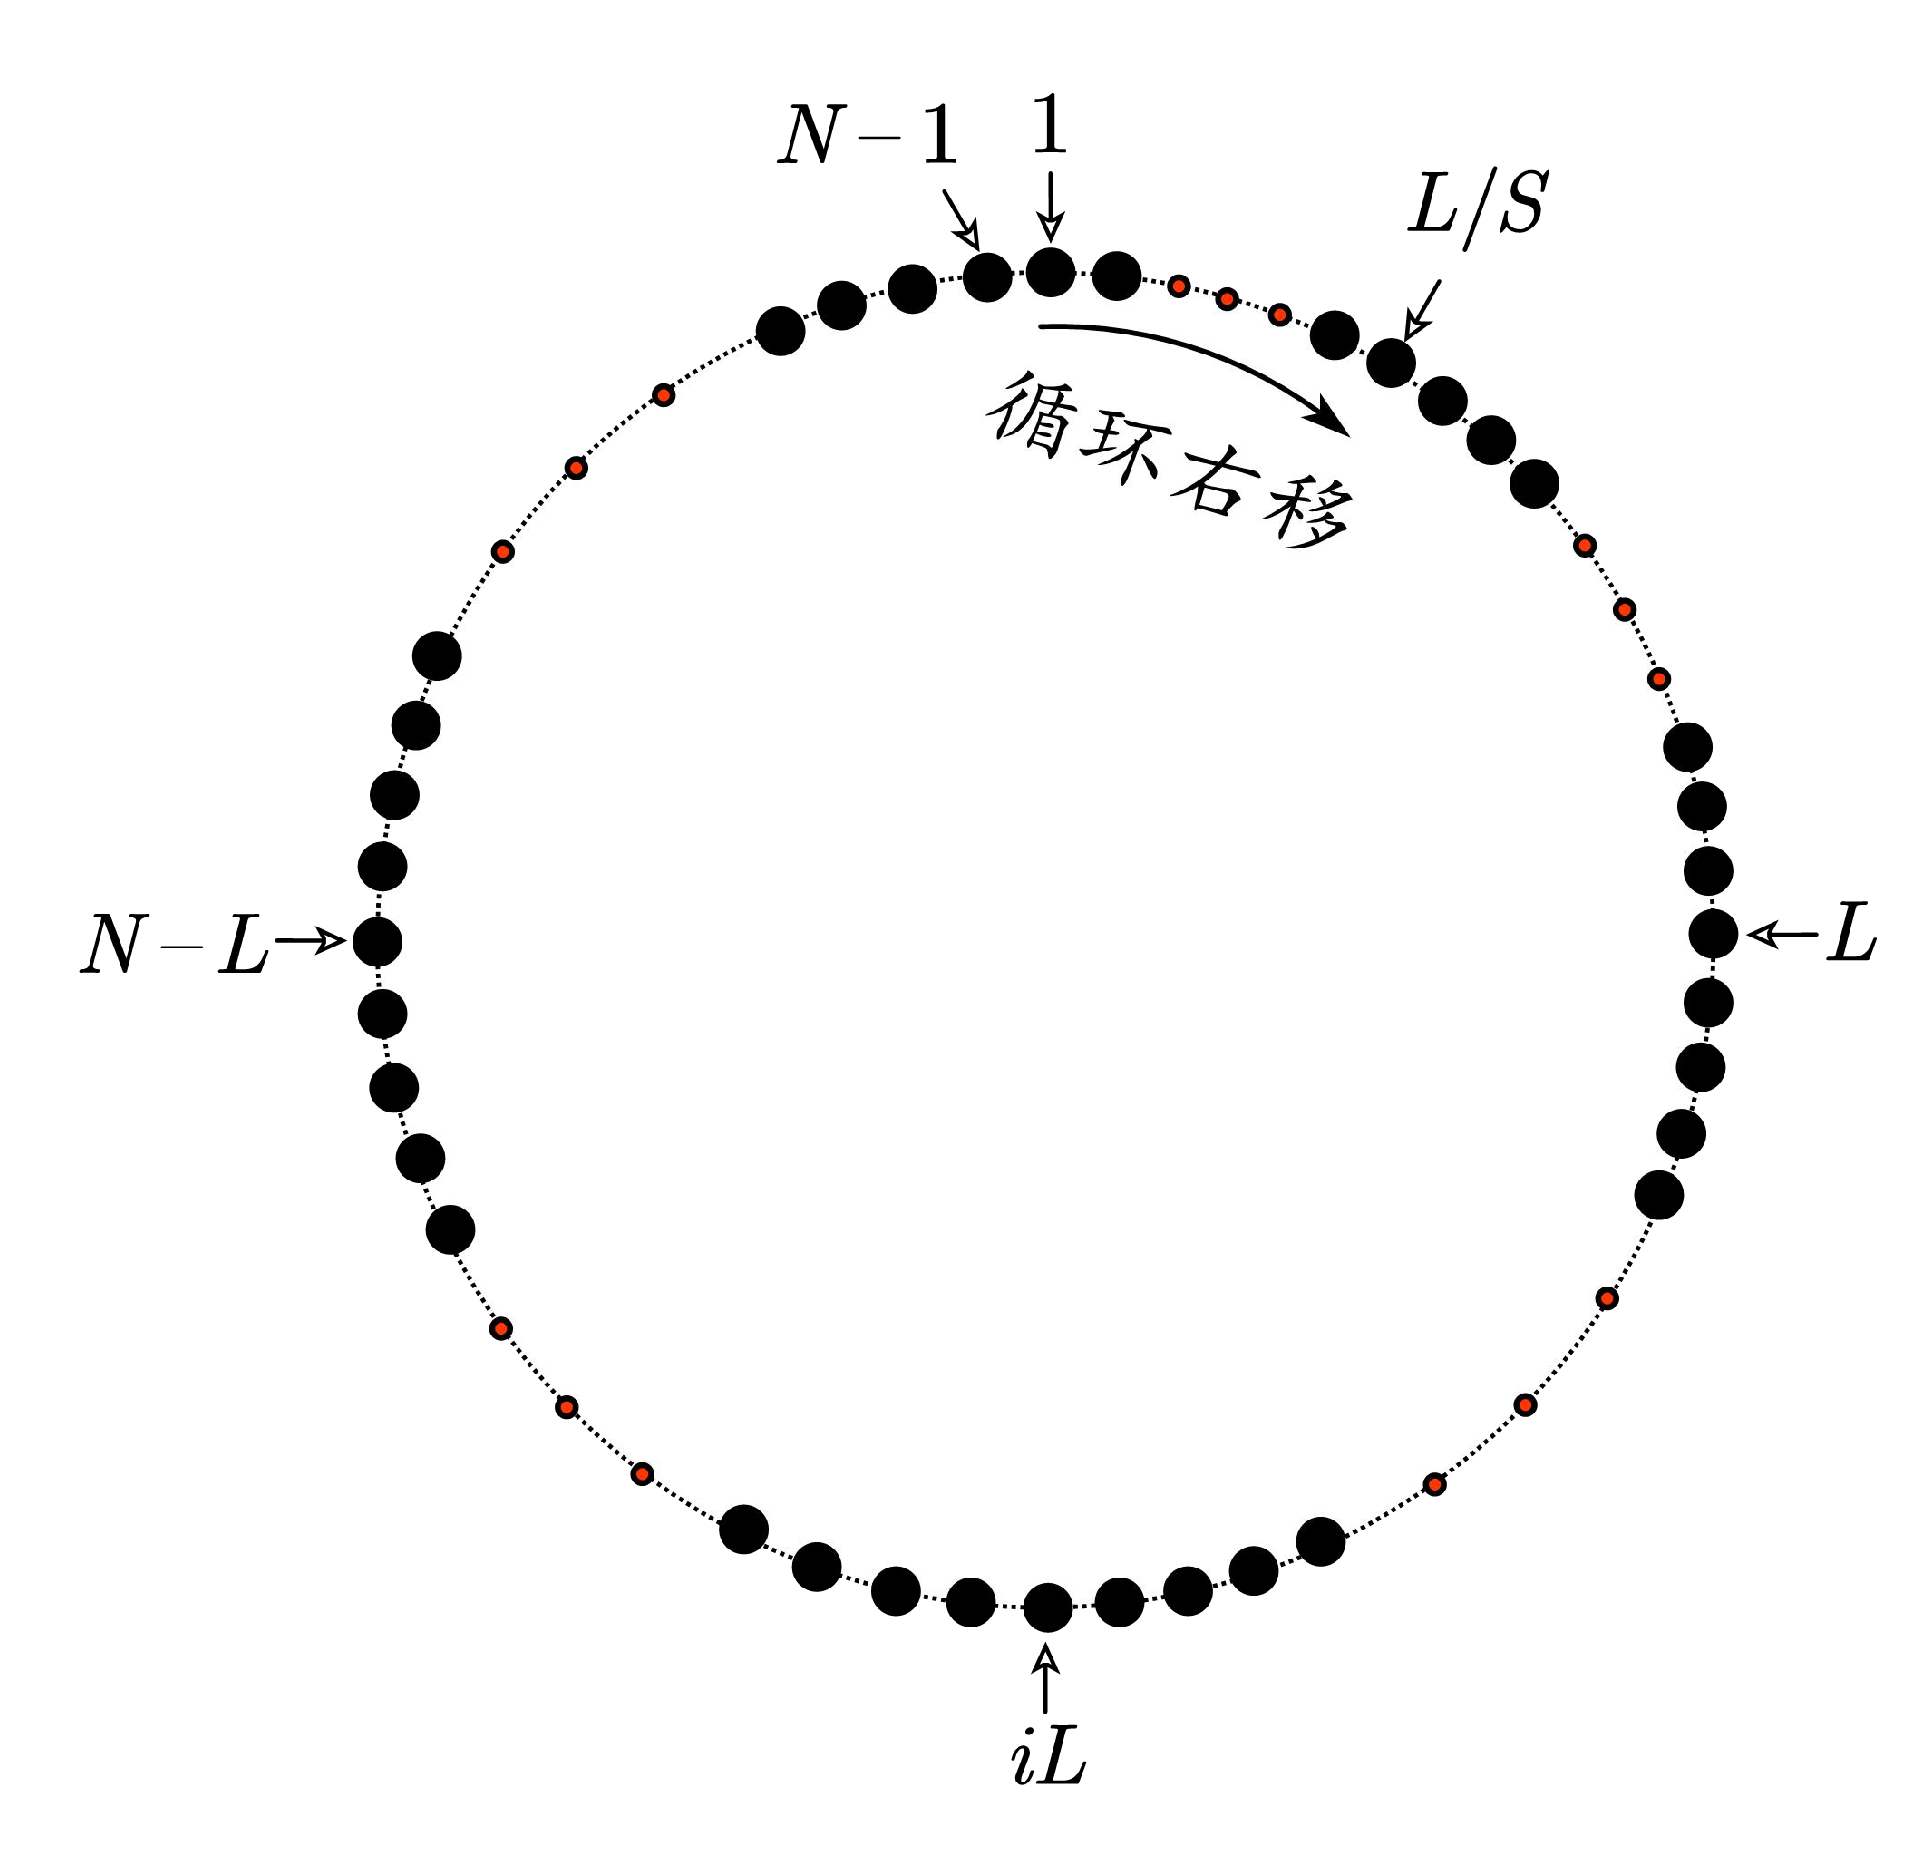
\includegraphics[width=.45\linewidth]{循环右移.pdf}
    \caption[循环扫描局部优化示意图]{循环扫描局部优化示意图}
    \label{fig:循环扫描局部优化示意图}
\end{figure}

\section{实验与讨论}
\label{sec:NS_Method:实验与讨论}

\subsection{实验设置及测试集}
\label{subsec:NS_Method:实验与讨论:测试集}
本节是对邻域结构生成方法进行实验,所有程序都是在Windows 10操作系统,2.4GHz的Intel i7 CPU和8G RAM的笔记本电脑上完成的。
\par
本实验使用的测试集都来自于DIMACS TSP竞赛\footnote{http://dimacs.rutgers.edu/archive/Challenges/TSP/}和TSPLIB\footnote{http://comopt.ifi.uni-heidelberg.de/software/TSPLIB95/}。包括了聚类型测试用例、均匀分布型测试用例、印刷电路板测试用例和真实地理位置测试用例,它们能够从各个方面体现算法生成的邻域结构的质量优劣,其具体信息如\autoref{tab:邻域结构测试集}~:
\begin{table}[htb]
    \caption[邻域结构测试集]{邻域结构测试集\label{tab:邻域结构测试集}}
    \begin{tabular}{llll}
        \toprule
        测试集类型 & 测试用例名称 & 节点数   & 权重类型 \\
        \midrule
        \multirow{5}[2]{*}{聚类型} & C1k   & 1000  & EUC\_2D \\
              & C3k   & 3162  & EUC\_2D \\
              & C10k  & 10000 & EUC\_2D \\
              & C31k  & 31623 & EUC\_2D \\
              & C100k & 100000 & EUC\_2D \\
        \midrule
        \multirow{5}[2]{*}{均匀分布型} & E1k   & 1000  & EUC\_2D \\
              & E3k   & 3162  & EUC\_2D \\
              & E10k  & 10000 & EUC\_2D \\
              & E31k  & 31623 & EUC\_2D \\
              & E100k & 100000 & EUC\_2D \\
        \midrule
        \multirow{2}[2]{*}{印刷电路板} & pla7397 & 7397  & CEIL\_2D \\
              & pla85900 & 85900 & CEIL\_2D \\
        \midrule
        真实地理位置 & brd14051 & 14051 & EUC\_2D \\
        \bottomrule
    \end{tabular}%
\end{table}
\par
在\autoref{tab:邻域结构测试集}~中,权重类型\cite{reinelt1995tsplib95}有两种,除了印刷电路板测试用例的权重类型是$CEIL\_2D$外,其他的测试用例的权重类型都为$EUC\_2D$,其计算公式如下:
\begin{itemize}
    \item $EUC\_2D$为二维欧几里得权重,设有两点及其坐标$v_i = (x_i, y_i)$和$v_j = (x_j, y_j)$,则边$e_{i,j}$的权重为:
    \vspace{-1.5em}
    \begin{align}
        \label{eq:EUC_2D}
        w_{i,j} = \lfloor \sqrt{(x_i-x_j)^2 + (y_i-y_j)^2} + 0.5 \rfloor .
    \end{align}
    \vspace{-1.5em}
    \item $EUC\_2D$为二维向上取整的欧几里得距离,设有两点及其坐标$v_i = (x_i, y_i)$和$v_j = (x_j, y_j)$,则边$e_{i,j}$的权重为:
    \vspace{-1.5em}
    \begin{align}
        \label{eq:CEIL_2D}
        w_{i,j} = \lceil \sqrt{(x_i-x_j)^2 + (y_i-y_j)^2} \rceil .
    \end{align}
\end{itemize}
\par
同时,为了测试算法的性能,本节主要用到了距离趋近度指标(章节~\ref{subsec:背景介绍:性能评价指标:距离趋近度指标})和最优边遗失率指标(章节~\ref{subsec:背景介绍:性能评价指标:最优边遗失率指标})来衡量算法生成的邻域结构的质量。

\subsection{meNS的质量及其生成算法的效率}
\label{subsec:NS_Method:实验与讨论:meNS质量及其生成算法的效率}
在本节中,将会验证meNS生成算法的执行效率及其生成meNS的质量。从章节~\ref{sec:NS_Method:邻域结构生成算法}~中可以知道,meNS生成算法是从大量的1MST中构造出一系列的Tour,这些Tour也可以被看作是问题的一个解。而meNS的最终质量也取决于这些被优化后的Tour的质量,因为meNS是由这些Tour的边构成的。从章节~\ref{subsec:NS_Method:邻域结构生成算法:meNS主框架}~中的算法\ref{alg:meNS生成算法主框架}~可以知道,meNS生成算法可以分成两个子部分:获取初始Tour和优化Tour。将1MST转变为Tour的操作就属于第一个部分,也正是这个部分不仅能提高最终生成邻域结构的质量,还能节省算法的时间,下面将比较meNS生成算法与随机初始Tour(raNS)的生成算法的效率和质量。
\begin{table}[htbp]
    \centering
    \caption{meNS生成算法的效率和质量 \label{tab:meNS生成算法的效率和质量}}
    \begin{threeparttable}
        \begin{tabular}{ll|cc|cc|cc}
            \toprule
            \multirow{2}[4]{*}{测试用例} & \multirow{2}[4]{*}{节点数} & \multicolumn{2}{c}{Time (s)} & \multicolumn{2}{c}{Gap (\%)} & \multicolumn{2}{c}{Degree}                          \\
            \cmidrule{3-8}               &                            & meNS                         & raNS                       & meNS                       & raNS  & meNS & raNS  \\
            \midrule
            C1k                      & 1000                       & 0.38                         & 0.46                         & 11.62                      & 20.70  & 6.9  & 6.5    \\
            C3k                        & 3162                       & 1.90                         & 2.05                         & 9.66                       & 17.37  & 6.6  & 6.9    \\
            C10k                       & 10000                      & 6.43                         & 7.95                         & 13.50                      & 37.05  & 6.6  & 7.0    \\
            C31k                       & 31623                      & 12.28                        & 15.85                        & 11.47                      & 41.77  & 6.3  & 7.0    \\
            C100k                      & 100000                     & 51.26                        & 53.00                        & 12.38                      & 43.38  & 7.6  & 7.1    \\
            \midrule
            E1k                       & 1000                       & 0.44                         & 0.40                         & 8.16                       & 14.28  & 6.8  & 7.1    \\
            E3k                        & 3162                       & 2.10                         & 2.26                         & 9.30                       & 17.37  & 6.7  & 7.4    \\
            E10k                       & 10000                      & 6.40                         & 7.50                         & 10.25                      & 20.12  & 7.0  & 7.6    \\
            E31k                       & 31623                      & 10.50                        & 15.01                        & 10.02                      & 21.93  & 6.6  & 7.8    \\
            E100k.0                      & 100000                     & 33.64                        & 51.81                        & 9.99                       & 22.90  & 6.5  & 7.8    \\
            \midrule
            pla7397                      & 7397                       & 1.80                         & 3.88                         & 9.82                       & 27.54  & 7.1  & 7.5    \\
            pla85900                     & 85900                      & 20.20                        & 37.94                        & 9.38                       & 27.00  & 7.0  & 7.9    \\
            \midrule
            brd14051                     & 14051                      & 6.42                         & 9.61                         & 8.27                       & 18.07  & 6.6  & 7.6    \\
            \bottomrule
        \end{tabular}
        \begin{tablenotes}
            \item meNS为meNS生成算法.
            \item raNS为随机初始Tour的生成算法.
        \end{tablenotes}
    \end{threeparttable}
\end{table}
\par
\autoref{tab:meNS生成算法的效率和质量}~展示的是meNS生成算法(简称meNS)与随机初始Tour的生成算法(简称raNS)的效率和质量。在\autoref{tab:meNS生成算法的效率和质量}~中比较了meNS与raNS的三项指标,分别是算法生成邻域结构的时间、算法最终优化后的Tour的平均Gap(距离趋近度)指标和算法生成的邻域结构的平均稀疏度(节点的度)。
\par
从\autoref{tab:meNS生成算法的效率和质量}~中可以看出,meNS在三项指标上都要优于raNS。在算法生成邻域结构的时间上,如\autoref{fig:meNS与raNS时间对比示意图}~所示,虽然meNS和raNS随着节点数的增加,其时间增长速度都远低于二次方时间复杂度的增长速度,但是meNS在多种类型的测试用例上所用的时间都比raNS要少,这是因为,meNS在算法的第一阶段用1MST生成了大量的优质初始Tour,这个操作不仅能够使得算法节省生成Tour的时间,还能够使得算法在第二阶段优化这些Tour的时候更快的收敛到理想值。而raNS是随机产生的初始Tour,这个操作虽然用时可能更少,生成的初始Tour的质量不一定高,这使得算法在第二阶段需要花费大量的时间来进一步优化这些质量并不好的Tour,这导致算法整体的时间过长。在算法最终优化的Tour的平均Gap指标上,meNS生成的Tour的平均Gap指标只有raNS的一半左右,说明meNS生成的Tour更接近最优Tour,这意味着用这些Tour来构造邻域结构会包含更多的最优Tour中的边。在算法生成的邻域结构的平均稀疏度上,meNS生成的邻域结构也比raNS生成的邻域结构更稀疏,并且这是算法生成邻域结构后未被修剪的数据,这说明meNS生成的邻域结构更加精简,算法在使用时能够更快的收敛。
\begin{figure}[htb]
    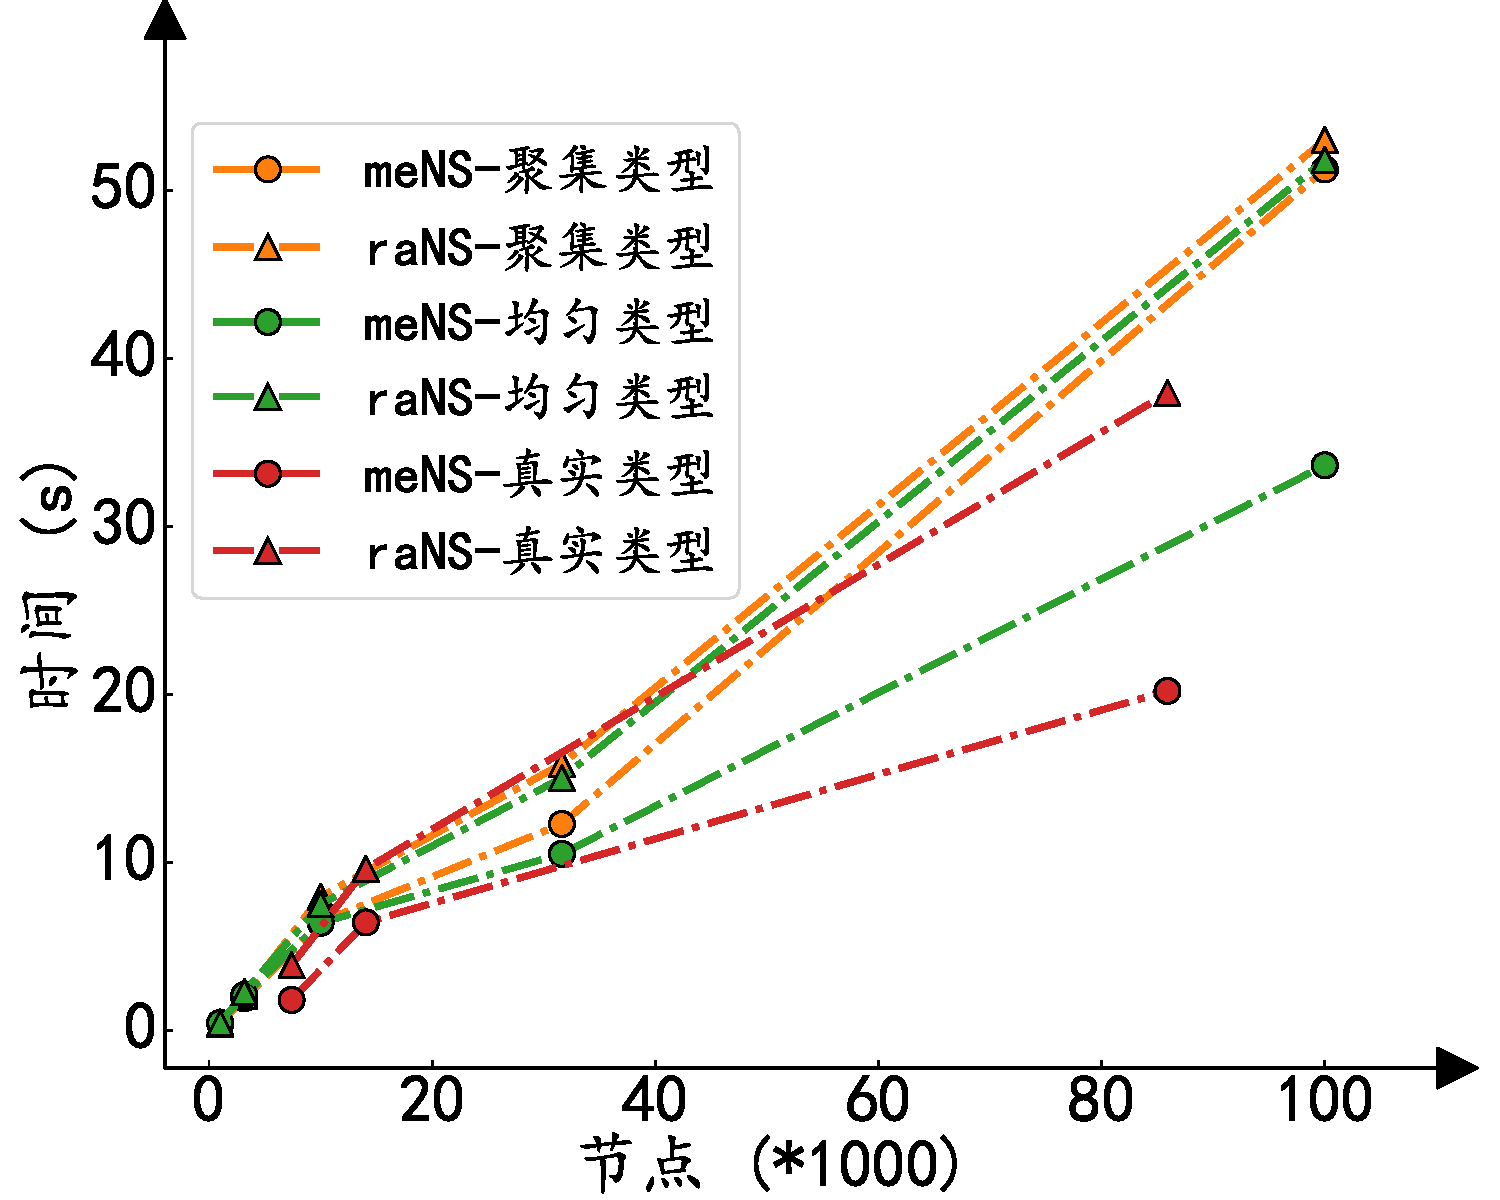
\includegraphics[width=.75\linewidth]{meNS时间对比.pdf}
    \caption[meNS与raNS时间对比示意图]{meNS与raNS时间对比示意图}
    \label{fig:meNS与raNS时间对比示意图}
\end{figure}

\subsection{meNS与其他邻域结构生成算法的比较}
\label{subsec:NS_Method:实验与讨论:meNS与其他邻域结构生成算法的比较}
在章节~\ref{subsec:NS_Method:实验与讨论:meNS质量及其生成算法的效率}~中,展示了meNS生成算法生成的未修剪的邻域结构的质量。在本节中,将会对比由meNS生成算法生成的修剪过的邻域结构与K最邻近(K-NN)、$\alpha$-nearest和三角剖分(Delaunay)算法生成的邻域结构的质量。由章节~\ref{subsec:NS_Method:邻域结构生成算法:meNS主框架}~中算法\ref{alg:meNS生成算法主框架}~可知,邻域结构在经过进一步的优化后,还需要进行修剪。因为邻域结构的稀疏度关乎到算法的运行速度,邻域结构越稀疏,算法的收敛的就越快。但是,邻域结构又不能太稀疏,因为这可能使得邻域结构中包含最优Tour的边变少,所以,在算法中,使邻域结构中的每个点只保留$M$条边的方式来进行邻域结构的修剪,在本文中,所有的邻域结构的最大保留边都设为$M=5$。
\setlength{\tabcolsep}{13pt}
\begin{longtable}[c]{llllll}
    \caption{meNS与K-NN、$\alpha$-nearest和Delaunay邻域结构生成算法的邻域结构质量对比}\label{tab:各算法表现}\\
    \toprule
	测试用例  & 指标  & meNS  & K-NN  & $\alpha$-nearest & Delaunay \\ 
    \midrule
	\endfirsthead
	\multicolumn{6}{c}{\nuaafontcaption 续表~\thetable\hskip1em meNS与K-NN、$\alpha$-nearest和三角剖分邻域结构生成算法的邻域结构质量对比}\\
	\toprule
	测试用例  & 指标  & meNS  & K-NN  & $\alpha$-nearest & Delaunay \\ 
    \midrule
	\endhead
	\hline
	\multicolumn{6}{r}{续下页}
	\endfoot
	\endlastfoot
    \multirow{4}[2]{*}{C1k}    & Preprocessing Time (s) & 1.7    & 1.18   & 2.74    & 0.96   \\
                & NS Degree       & 4.6    & 4.7    & 5       & 5      \\
                & Missing (\%)              & 0.2000  & 0.2000  & 0.4000  & 0.5000  \\
                & LKH Gap (\%)           & 0.5438 & 0.5438 & 0.5438  & 0.5438 \\
    \midrule
    \multirow{4}[2]{*}{C3k}    & Preprocessing Time (s) & 7.43   & 4.99   & 19.06   & 3.43   \\
                & NS Degree       & 4.6    & 4.9    & 5       & 5      \\
                & Missing (\%)               & 0.1898  & 0.1581  & 0.4111  & 0.2530  \\
                & LKH Gap (\%)           & 0.6179 & 0.7107 & 0.6179  & 0.6179 \\
    \midrule
    \multirow{4}[2]{*}{C10k}   & Preprocessing Time (s) & 33.77  & 20.26  & 82.09   & 15.54  \\
                & NS Degree       & 4.6    & 4.8    & 5       & 5      \\
                & Missing (\%)               & 0.4400  & 0.1700  & 0.3200  & 0.2900  \\
                & LKH Gap (\%)           & 0.6688 & 0.7141 & 0.7966  & 0.7412 \\
    \midrule
    \multirow{4}[2]{*}{C31k}   & Preprocessing Time (s) & 119.26 & 83.12  & 506.62  & 63.95  \\
                & NS Degree       & 4.6    & 4.8    & 5       & 5      \\
                & Missing (\%)               & 0.2245  & 0.1328  & 0.3731  & 0.3384  \\
                & LKH Gap (\%)           & 0.5183 & 0.7978 & 1.7965  & 0.8065 \\
    \midrule
    \multirow{4}[2]{*}{C100k}  & Preprocessing Time (s) & 888.83 & 358.82 & 5140.05 & 323.03 \\
                & NS Degree       & 4.7    & 4.8    & 5       & 5      \\
                & Missing (\%)               & 0.13  & 0.173 & 0.363 & 0.353 \\
                & LKH Gap (\%)           & 0.1919 & 0.8343 & 1.2847  & 1.5998 \\
    \midrule
    \multirow{4}[2]{*}{E1k}    & Preprocessing Time (s) & 1.71   & 1.12   & 2.72    & 0.75   \\
                & NS Degree       & 4.5    & 4.8    & 5       & 4      \\
                & Missing (\%)               & 0.2000  & 0.2000  & 0.3000  & 2.8000  \\
                & LKH Gap (\%)           & 0.7677 & 0.7967 & 0.7677  & 1.012  \\
    \midrule
    \multirow{4}[2]{*}{E3k}    & Preprocessing Time (s) & 7.87   & 5.17   & 12.37   & 3.11   \\
                & NS Degree       & 4.6    & 4.9    & 3.1     & 3.8    \\
                & Missing (\%)               & 0.2846  & 0.2214  & 2.0873  & 1.3599  \\
                & LKH Gap (\%)           & 0.7138 & 0.7107 & 1.057   & 0.8482 \\
    \midrule
    \multirow{4}[2]{*}{E10k}   & Preprocessing Time (s) & 32.82  & 20.25  & 84.12   & 15.17  \\
                & NS Degree       & 4.6    & 4.9    & 4.2     & 4.9    \\
                & Missing (\%)               & 0.1600  & 0.0900  & 0.4500  & 0.1500  \\
                & LKH Gap (\%)           & 0.7103 & 0.7166 & 0.7481  & 0.7104 \\
    \midrule
    \multirow{4}[2]{*}{E31k}   & Preprocessing Time (s) & 112.95 & 73.63  & 497.43  & 74.01  \\
                & NS Degree       & 4.6    & 4.9    & 5       & 5      \\
                & Missing (\%)              & 0.1708  & 0.1202  & 0.2340  & 0.2150  \\
                & LKH Gap (\%)           & 0.3615 & 0.6463 & 0.6505  & 0.6549 \\
    \midrule
    \multirow{4}[2]{*}{E100k}  & Preprocessing Time (s) & 626.55 & 382.07 & 3349.24 & 323.62 \\
                & NS Degree       & 4.6    & 4.9    & 5       & 5      \\
                & Missing (\%)               & 0.1920  & 0.1220  & 0.2770  & 0.2230  \\
                & LKH Gap (\%)           & 0.4078 & 0.6664 & 0.6687  & 0.6658 \\
    \midrule
    \multirow{4}[2]{*}{pla7397}  & Preprocessing Time (s) & 9.82   & 12.17  & 41.33   & 11.38  \\
                & NS Degree       & 4.4    & 4.9    & 4.9     & 4.9    \\
                & Missing (\%)               & 0.1352  & 0.1622  & 0.2433  & 0.2433  \\
                & LKH Gap (\%)           & 0.586  & 0.5806 & 0.5842  & 0.5806 \\
    \midrule
    \multirow{4}[2]{*}{pla85900} & Preprocessing Time (s) & 432.86 & 337.45 & 1789.22 & 404.99 \\
                & NS Degree       & 4.5    & 5      & 4.8     & 4.8    \\
                & Missing (\%)               & 0.1630  & 0.0827  & 0.1281  & 0.1292  \\
                & LKH Gap (\%)           & 0.4701 & 0.4468 & 0.4774  & 0.4665 \\
    \midrule
    \multirow{4}[2]{*}{brd14051} & Preprocessing Time (s) & 43.66  & 32.52  & 125.29  & 26.7   \\
                & NS Degree       & 4.7    & 5      & 5       & 5      \\
                & Missing (\%)               & 0.0641  & 0.0925  & 0.1139  & 0.1139  \\
                & LKH Gap (\%)           & 0.4877 & 0.4855 & 0.4889  & 0.4883 \\
    \bottomrule
\end{longtable}
\par
\autoref{tab:各算法表现}~展示的是meNS与K-NN、$\alpha$-nearest和Delaunay算法生成的邻域结构的对比数据,并且在\autoref{tab:各算法表现}~中比较了各个算法生成的邻域结构在LKH算法\cite{helsgaun2000effective}(目前解决大型TSP问题最优秀的算法之一)中的表现,同时统计了各算法在生成邻域结构的时间(LKH预处理时间,Preprocessing Time)、邻域结构的稀疏度(NS Degree)、最优边遗失率(Missing)和LKH最终解的距离趋近度(LKH Gap)四项指标数据。
\par
从\autoref{tab:各算法表现}~可以看出,在Preprocessing Time指标数据上,使用Delaunay生成的邻域结构耗费的时间比其他算法生成邻域结构花费的时间都要少,因为Delaunay算法采用分治的思想对整个图进行三角剖分,能够在$O(nlogn)$的时间复杂度内完成邻域结构的构建,但是Delaunay只能在二维坐标测试问题上有效生成邻域结构,当测试问题的坐标维度高于二维时,Delaunay算法就难以保持其高效性且算法会变得及其复杂。而K-NN和$\alpha$-nearest算法都是$O(n^2)$的时间复杂度,所以在构造邻域结构花费的时间最多,meNS生成算法构造邻域结构花费的时间介于Delaunay和K-NN、$\alpha$-nearest算法构造邻域结构花费的时间之间,从侧面也可以证明meNS生成算法的时间复杂度是低于二次方时间复杂度的。\autoref{fig:meNS和其他算法生成邻域结构的时间示意图}~展示的是meNS生成算法和其他算法在不同类型测试用例构造邻域结构的时间示意图,从图中也能够得看出,meNS生成算法的高效性。
\begin{figure}[htb]
    \subfloat[聚类型 \label{subfig:聚类型}]{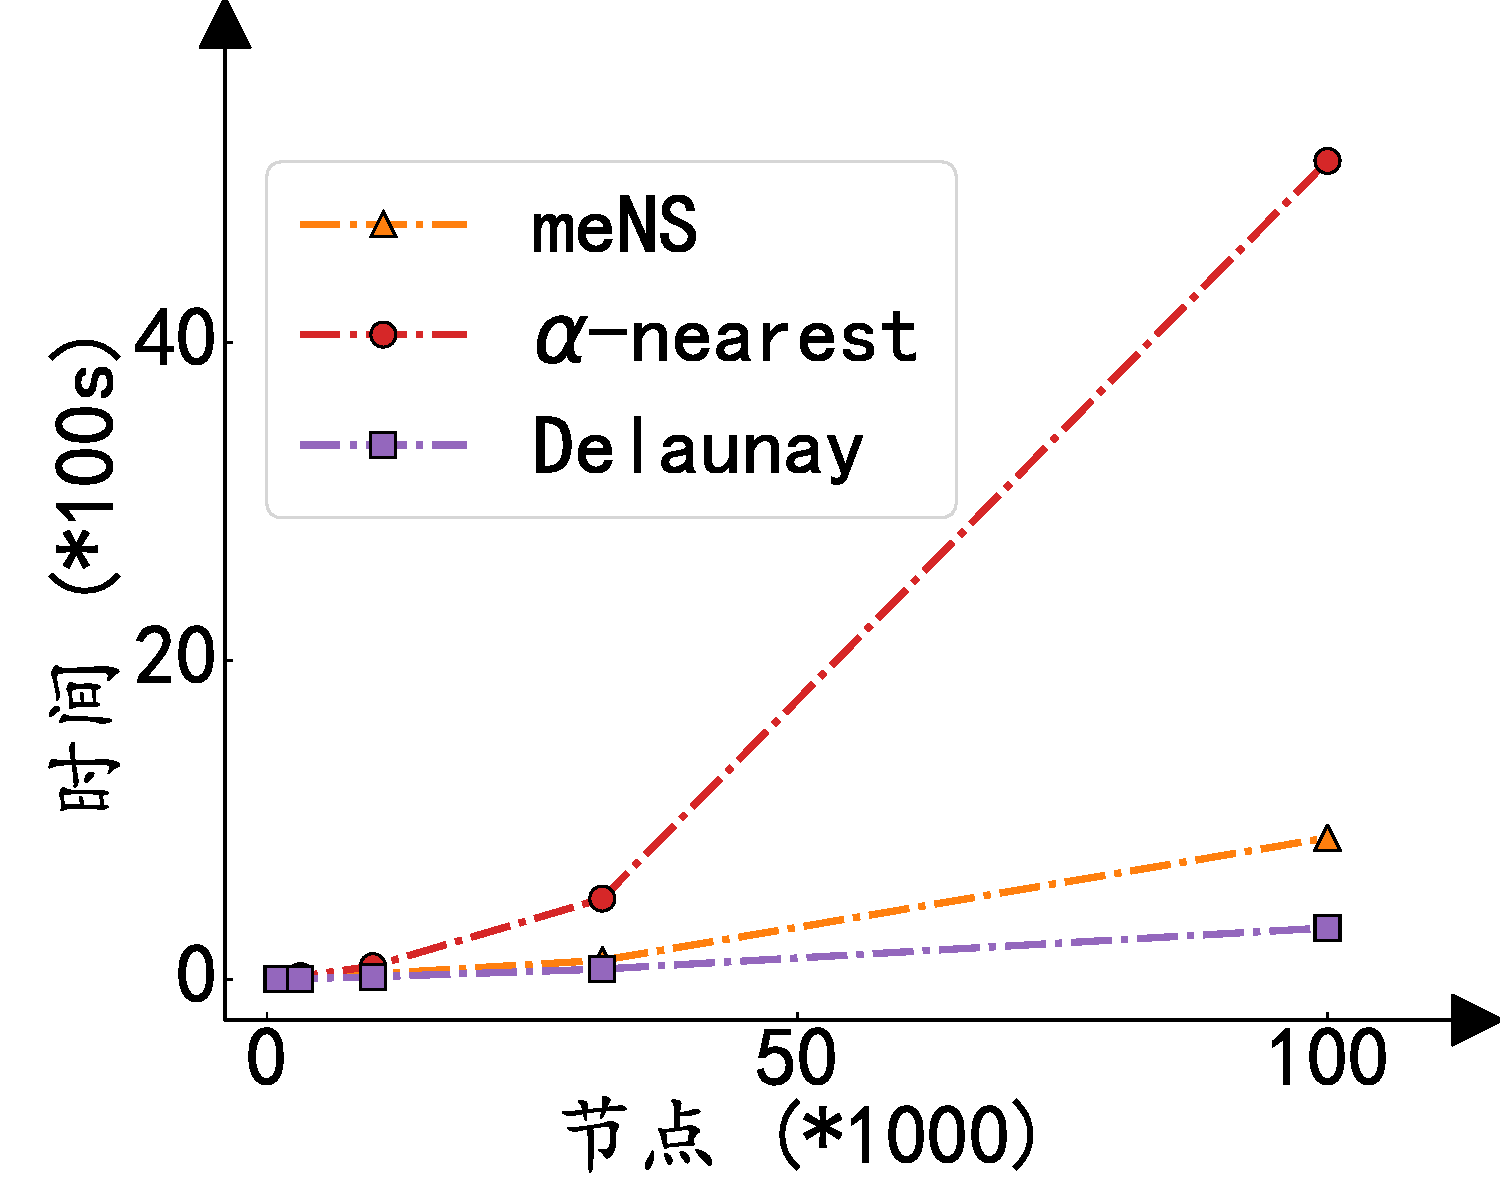
\includegraphics[width=.33\linewidth]{聚类型.pdf}}
    \subfloat[均匀分布型 \label{subfig:均匀分布型}]{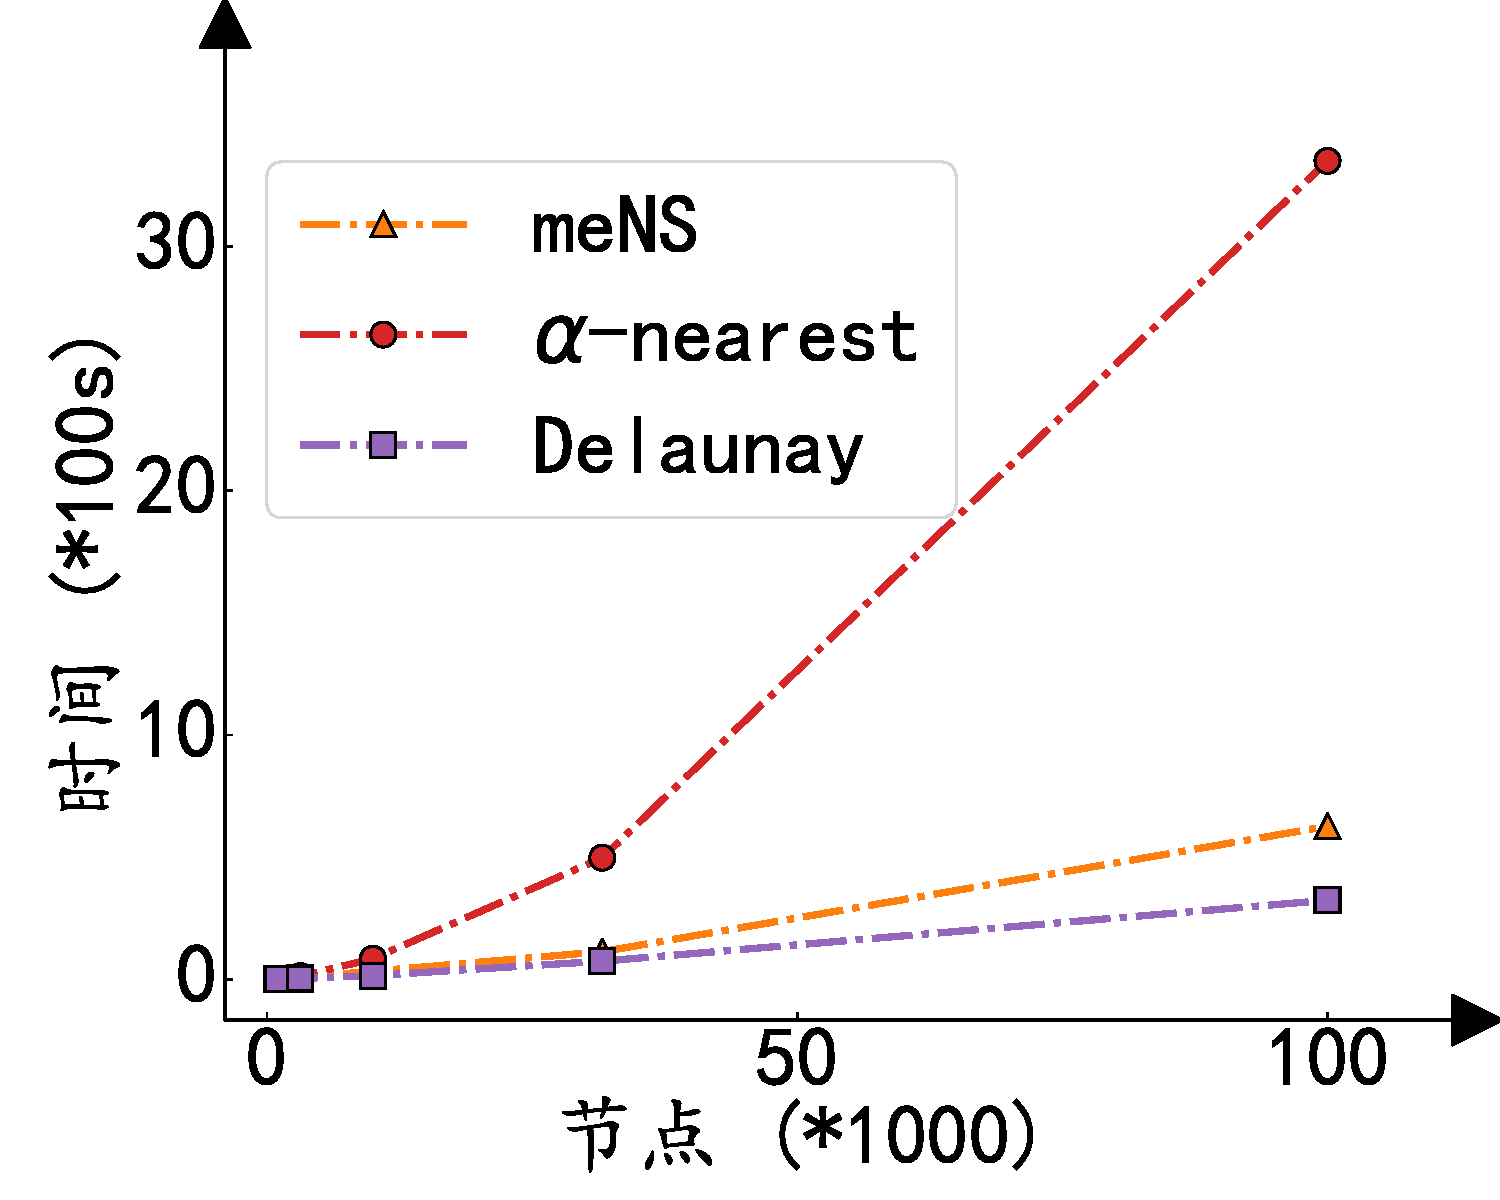
\includegraphics[width=.33\linewidth]{均匀分布型.pdf}}
    \subfloat[真实数据 \label{subfig:真实数据}]{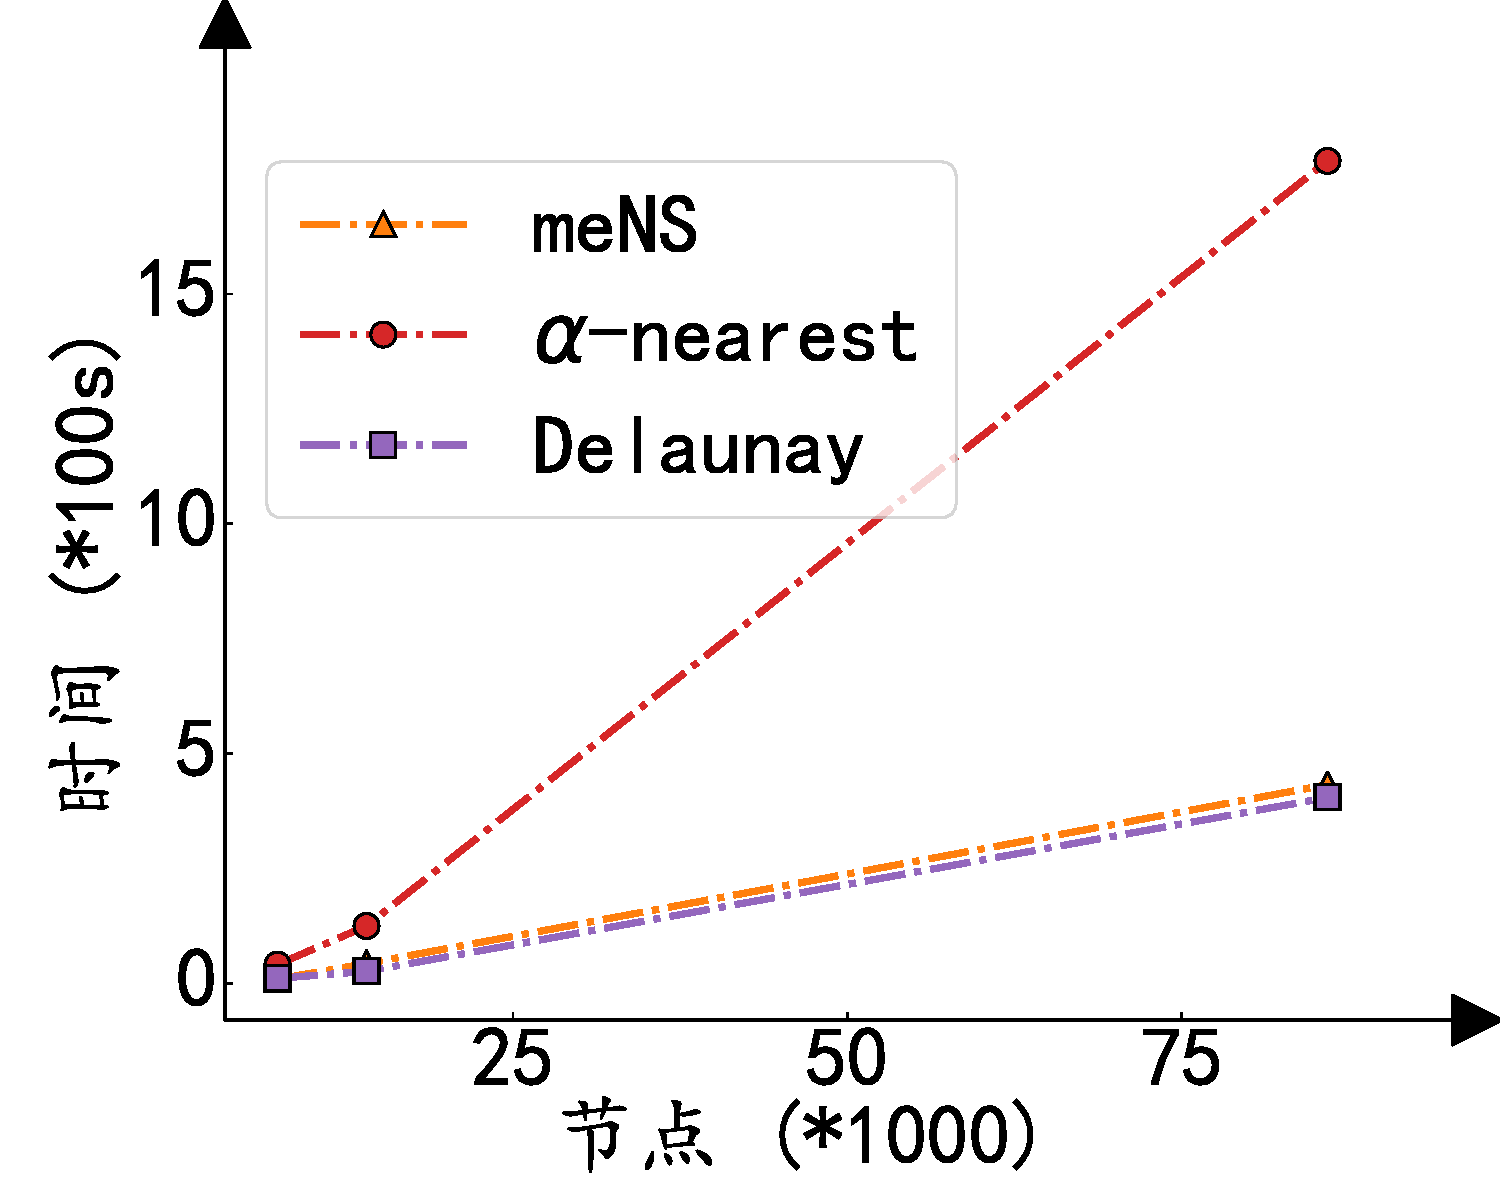
\includegraphics[width=.33\linewidth]{真实数据.pdf}}
    \caption[meNS和其他算法生成邻域结构的时间示意图]{meNS和其他算法生成邻域结构的时间示意图}
    \label{fig:meNS和其他算法生成邻域结构的时间示意图}
\end{figure}
\par
在将各算法生成的邻域结构正式应用到LKH算法中之前,还需要对邻域结构进行修剪,以保证邻域结构的稀疏度。在本文中,邻域结构在修剪后,每个点最多只保留$M=5$条边作为其邻域。因此,从\autoref{tab:各算法表现}~中可以知道,在NS Degree指标数据上,所有的数值都不超过5,这是就是对邻域结构修剪的结果,但是,在各数值上仍然能够得出,meNS生成算法的邻域结构修剪后要比其他生成算法修剪后的邻域结构更加稀疏,这使得该邻域结构用在求解算法中会收敛的更快,\autoref{fig:各算法在聚类型用例C10K生成的邻域结构}~、\autoref{fig:各算法在聚类型用例C10K生成的邻域结构}~,\autoref{fig:各算法在印刷电路板测试用例pla7397生成的邻域结构}~和\autoref{fig:各算法在真实地理位置测试用例brd14051生成的邻域结构}~中分别展示了各算法对于不同类型的测试用例生成的邻域结构修剪后的部分示意图。
\begin{figure}[!htb]
    \subfloat[meNS]{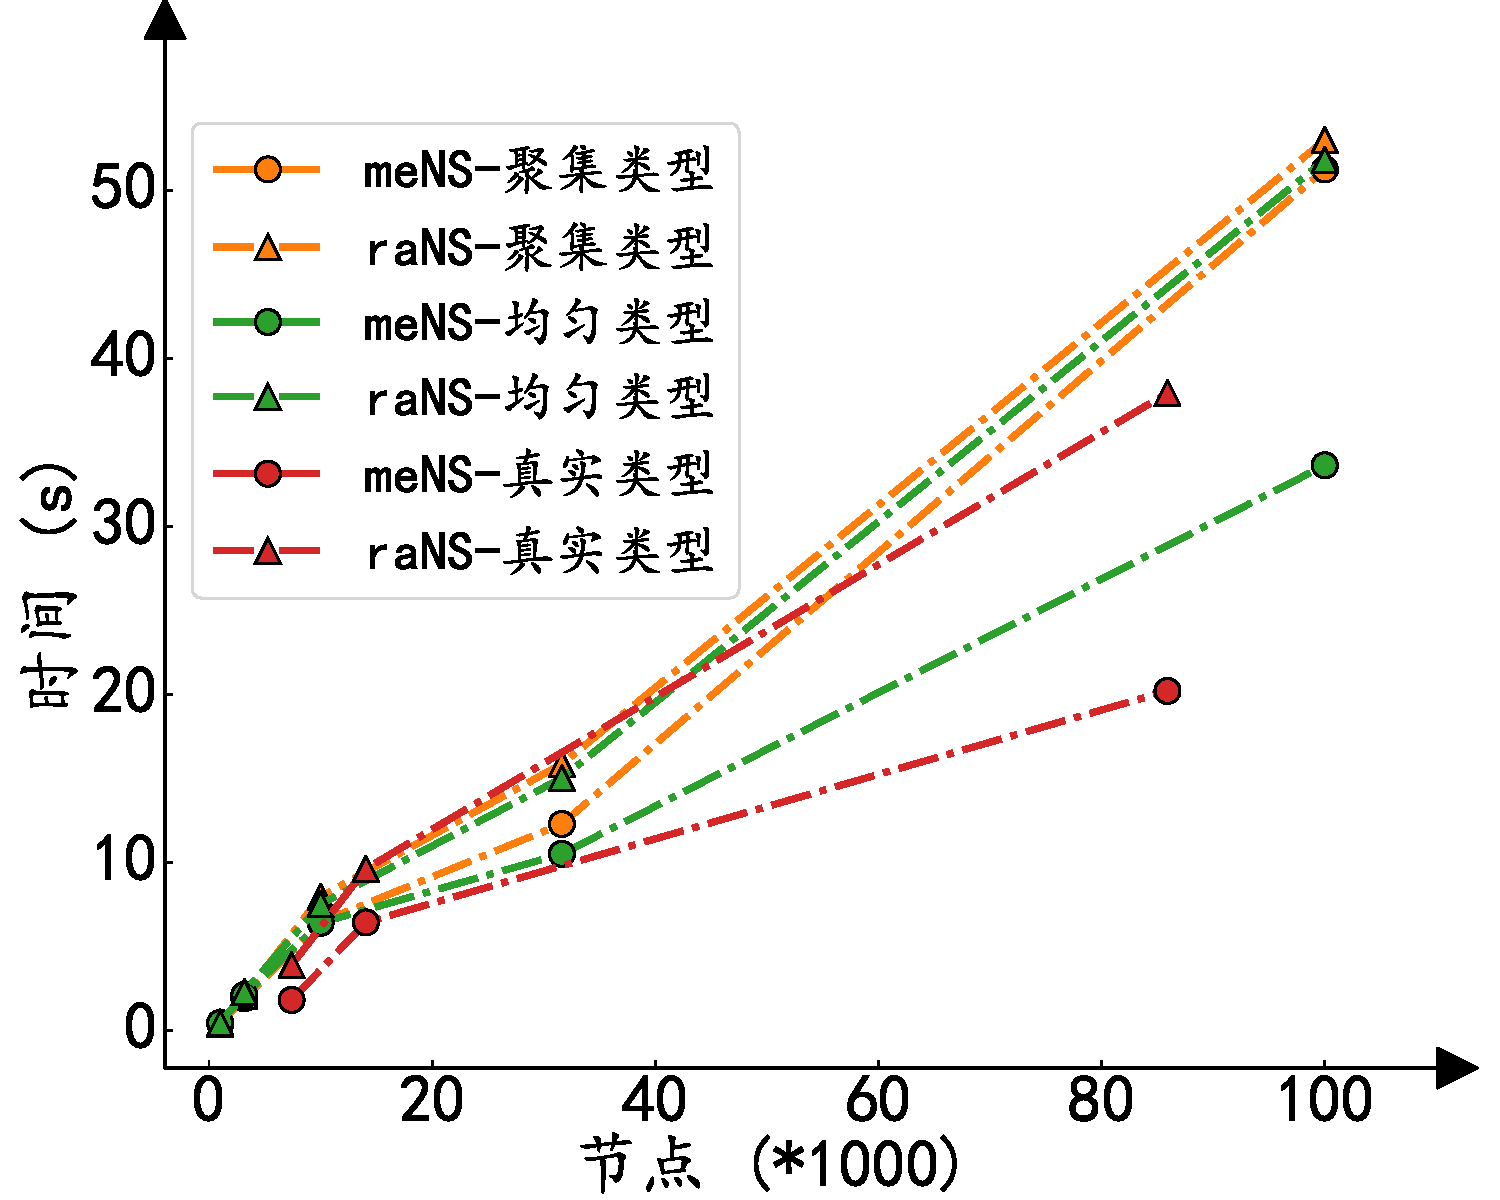
\includegraphics[width=.3\linewidth]{meNS时间对比.pdf}}
    \subfloat[K-NN]{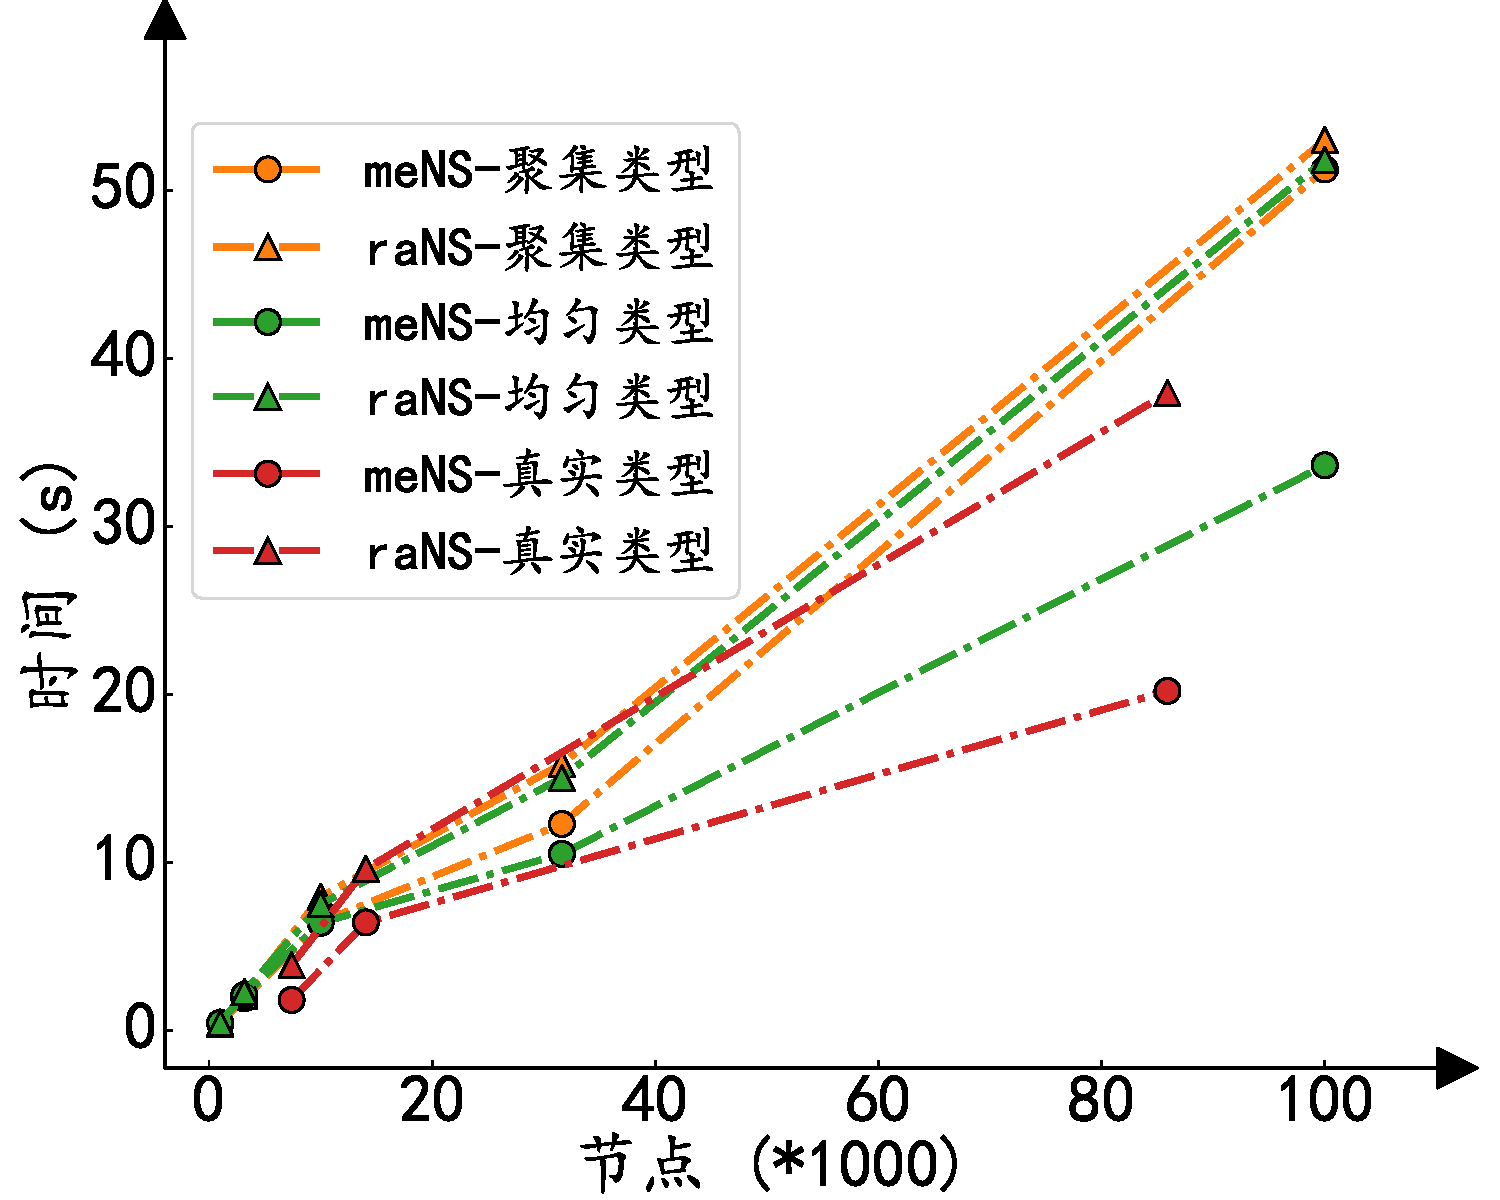
\includegraphics[width=.3\linewidth]{meNS时间对比.pdf}} \\
    \subfloat[$\alpha$-nearest]{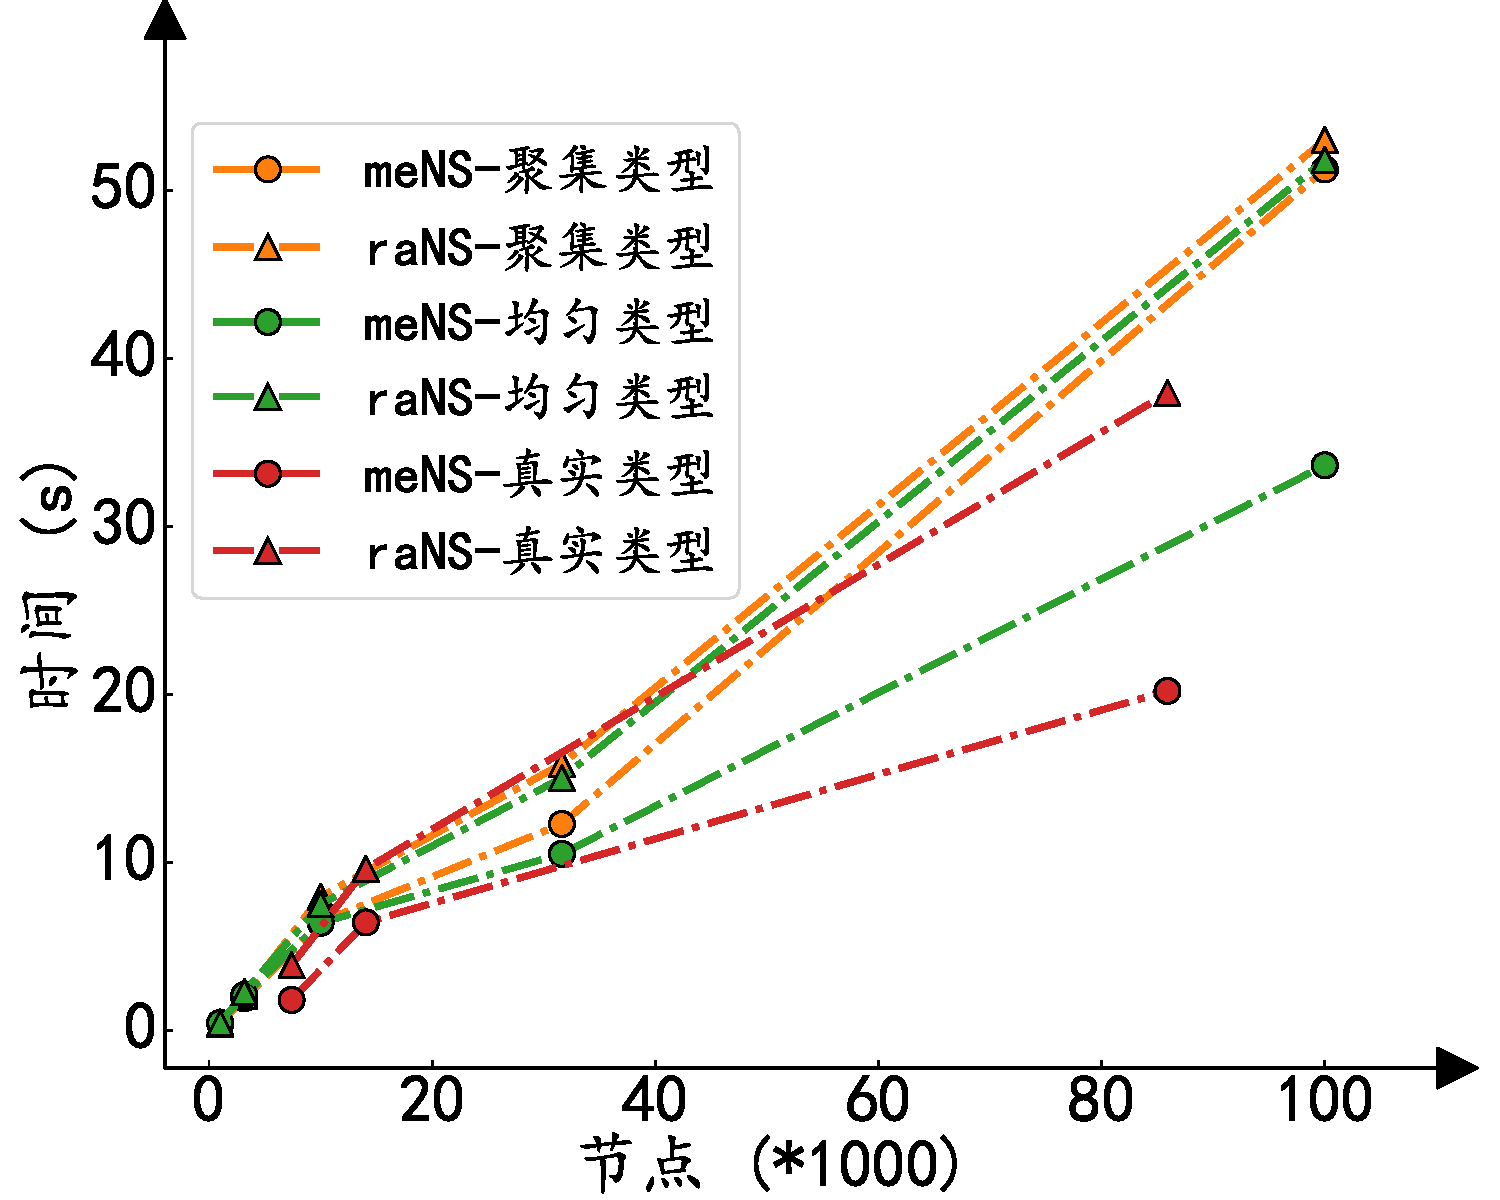
\includegraphics[width=.3\linewidth]{meNS时间对比.pdf}}
    \subfloat[Delaunay]{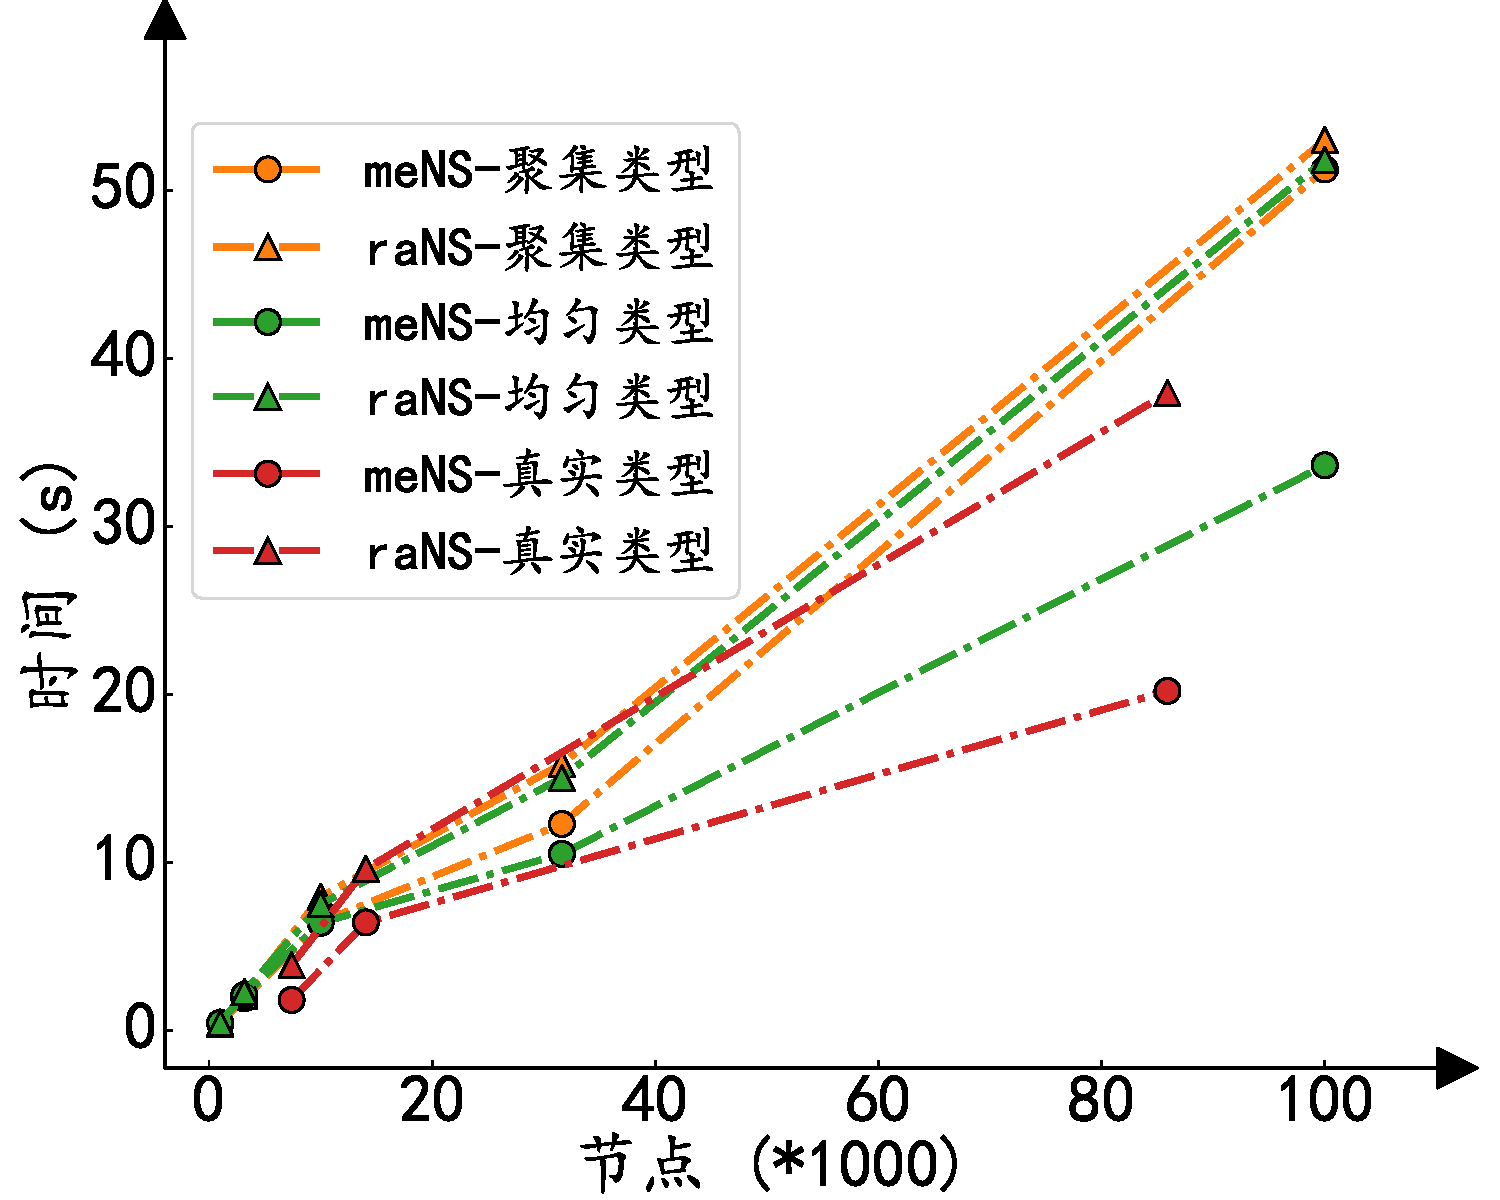
\includegraphics[width=.3\linewidth]{meNS时间对比.pdf}}
    \caption[各算法在聚类型用例$C10K$生成的邻域结构]{各算法在聚类型用例$C10K$生成的邻域结构}
    \label{fig:各算法在聚类型用例C10K生成的邻域结构}
\end{figure}
\begin{figure}[!h]
    \subfloat[meNS]{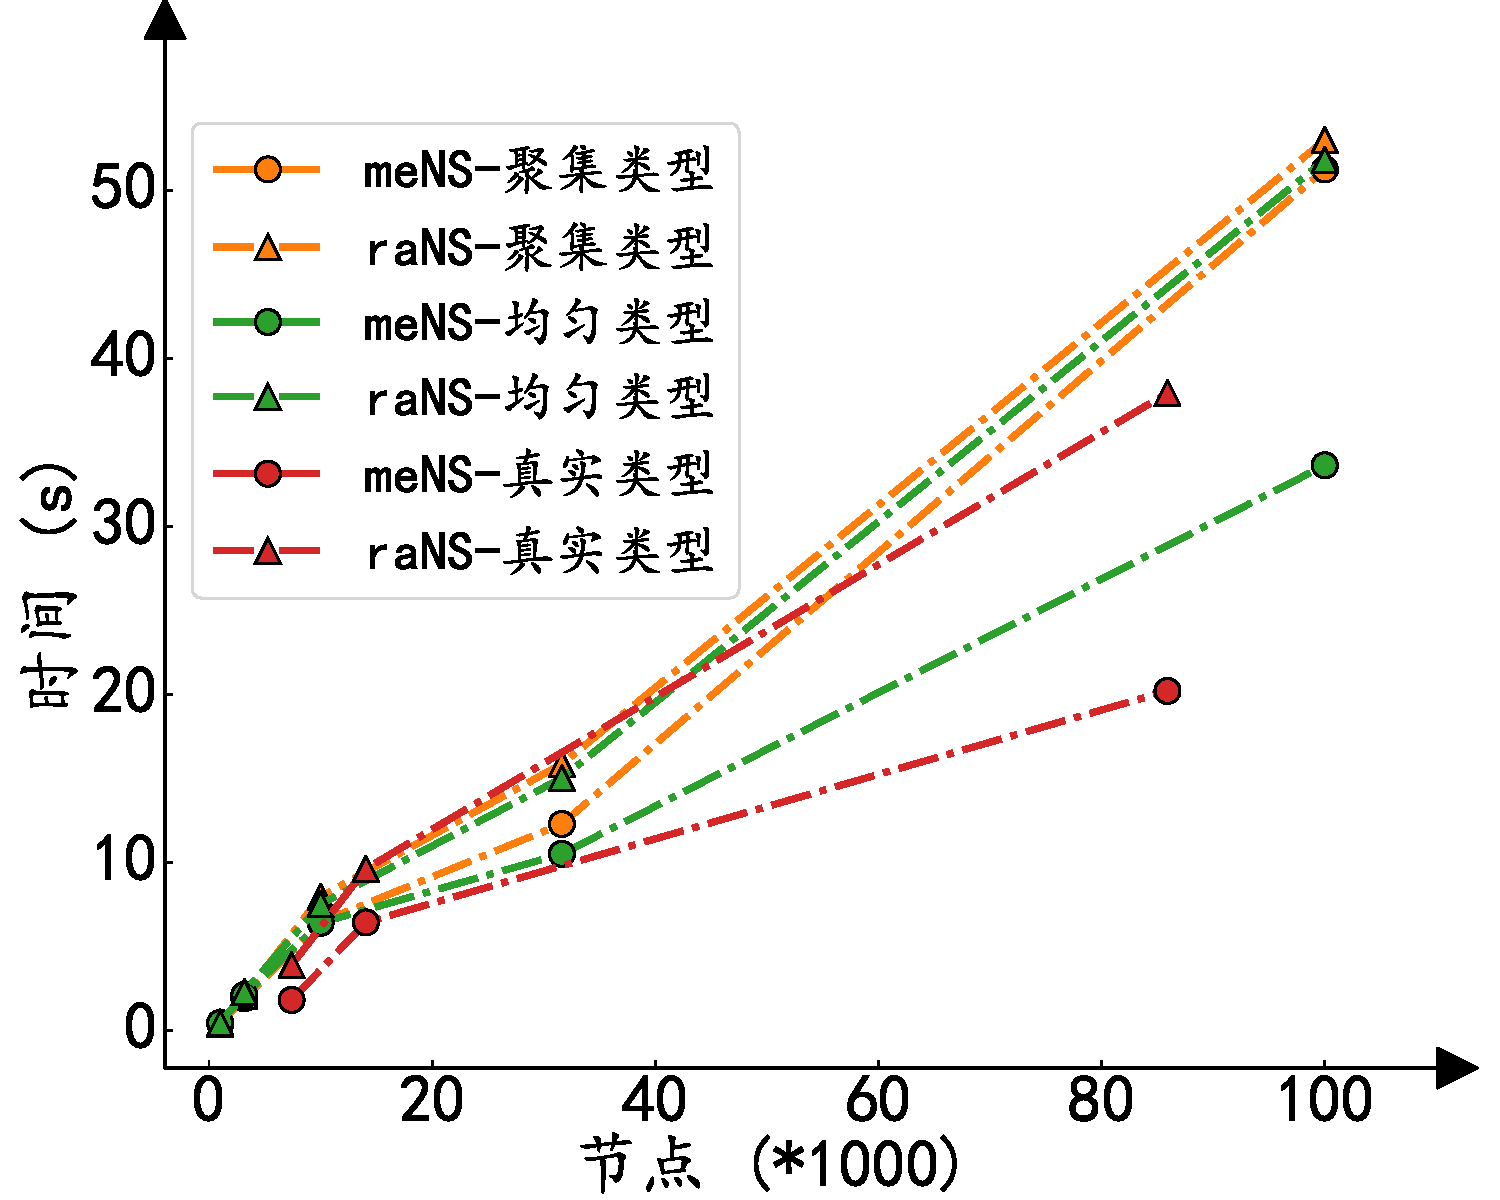
\includegraphics[width=.3\linewidth]{meNS时间对比.pdf}}
    \subfloat[K-NN]{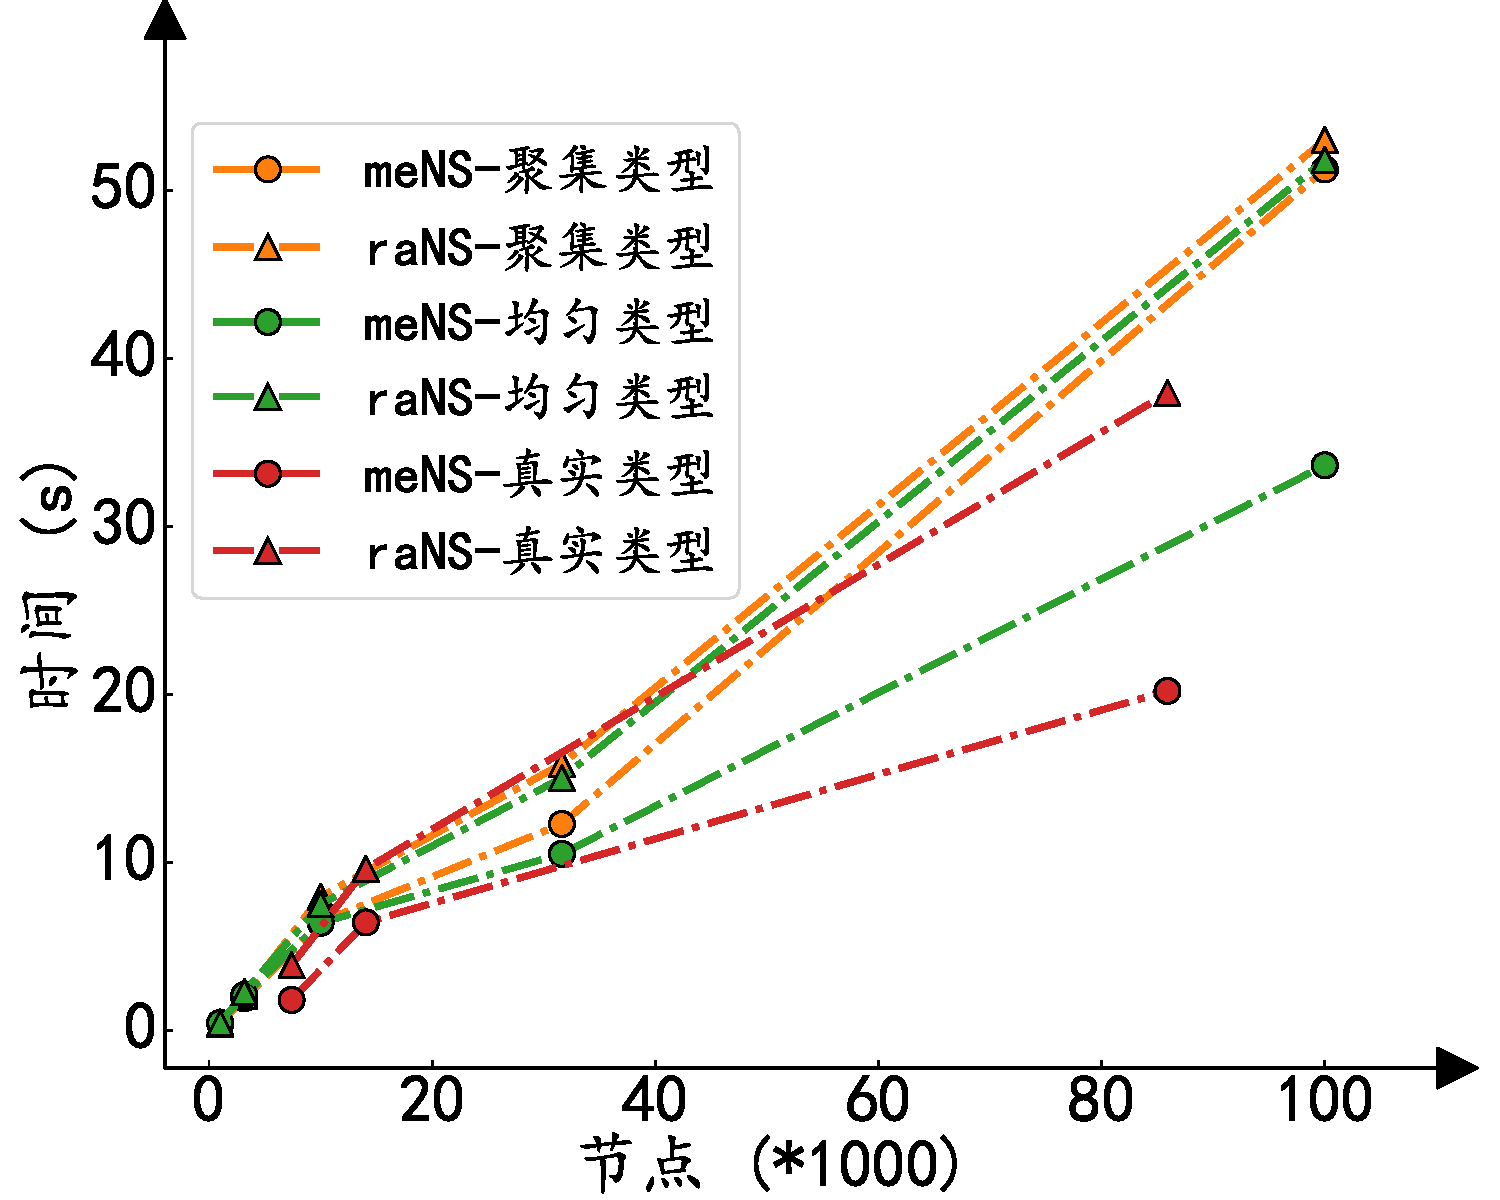
\includegraphics[width=.3\linewidth]{meNS时间对比.pdf}} \\
    \subfloat[$\alpha$-nearest ]{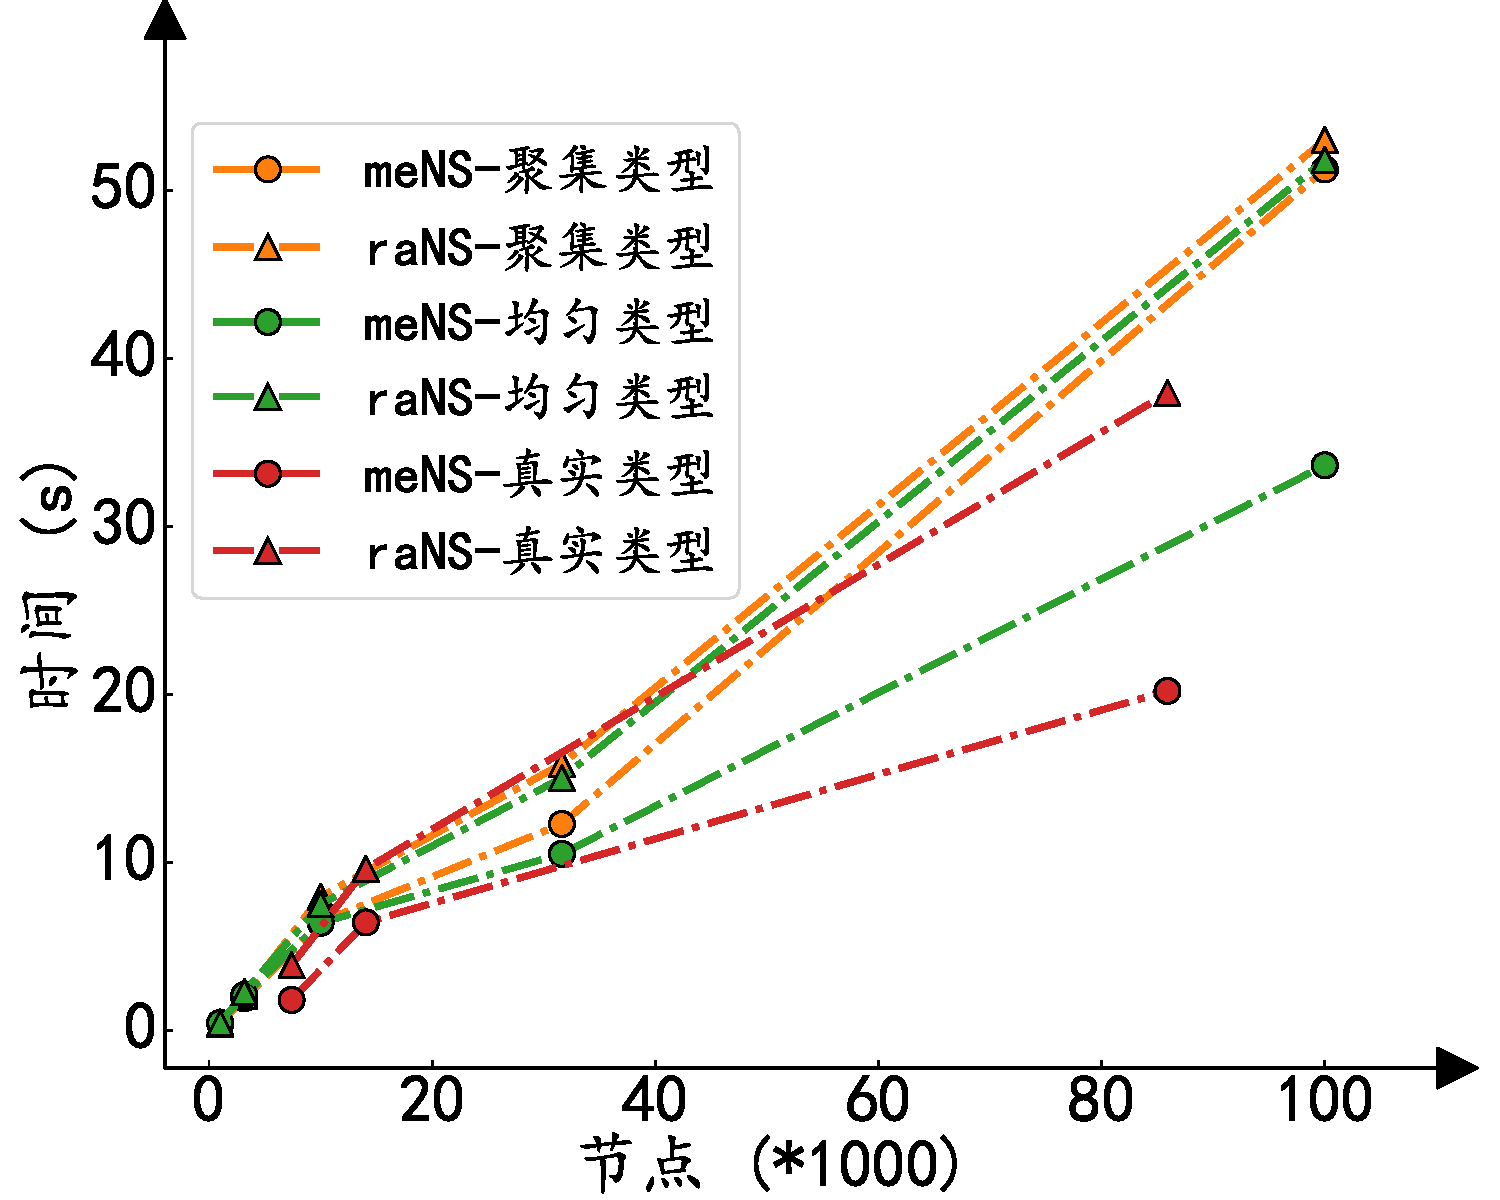
\includegraphics[width=.3\linewidth]{meNS时间对比.pdf}}
    \subfloat[Delaunay]{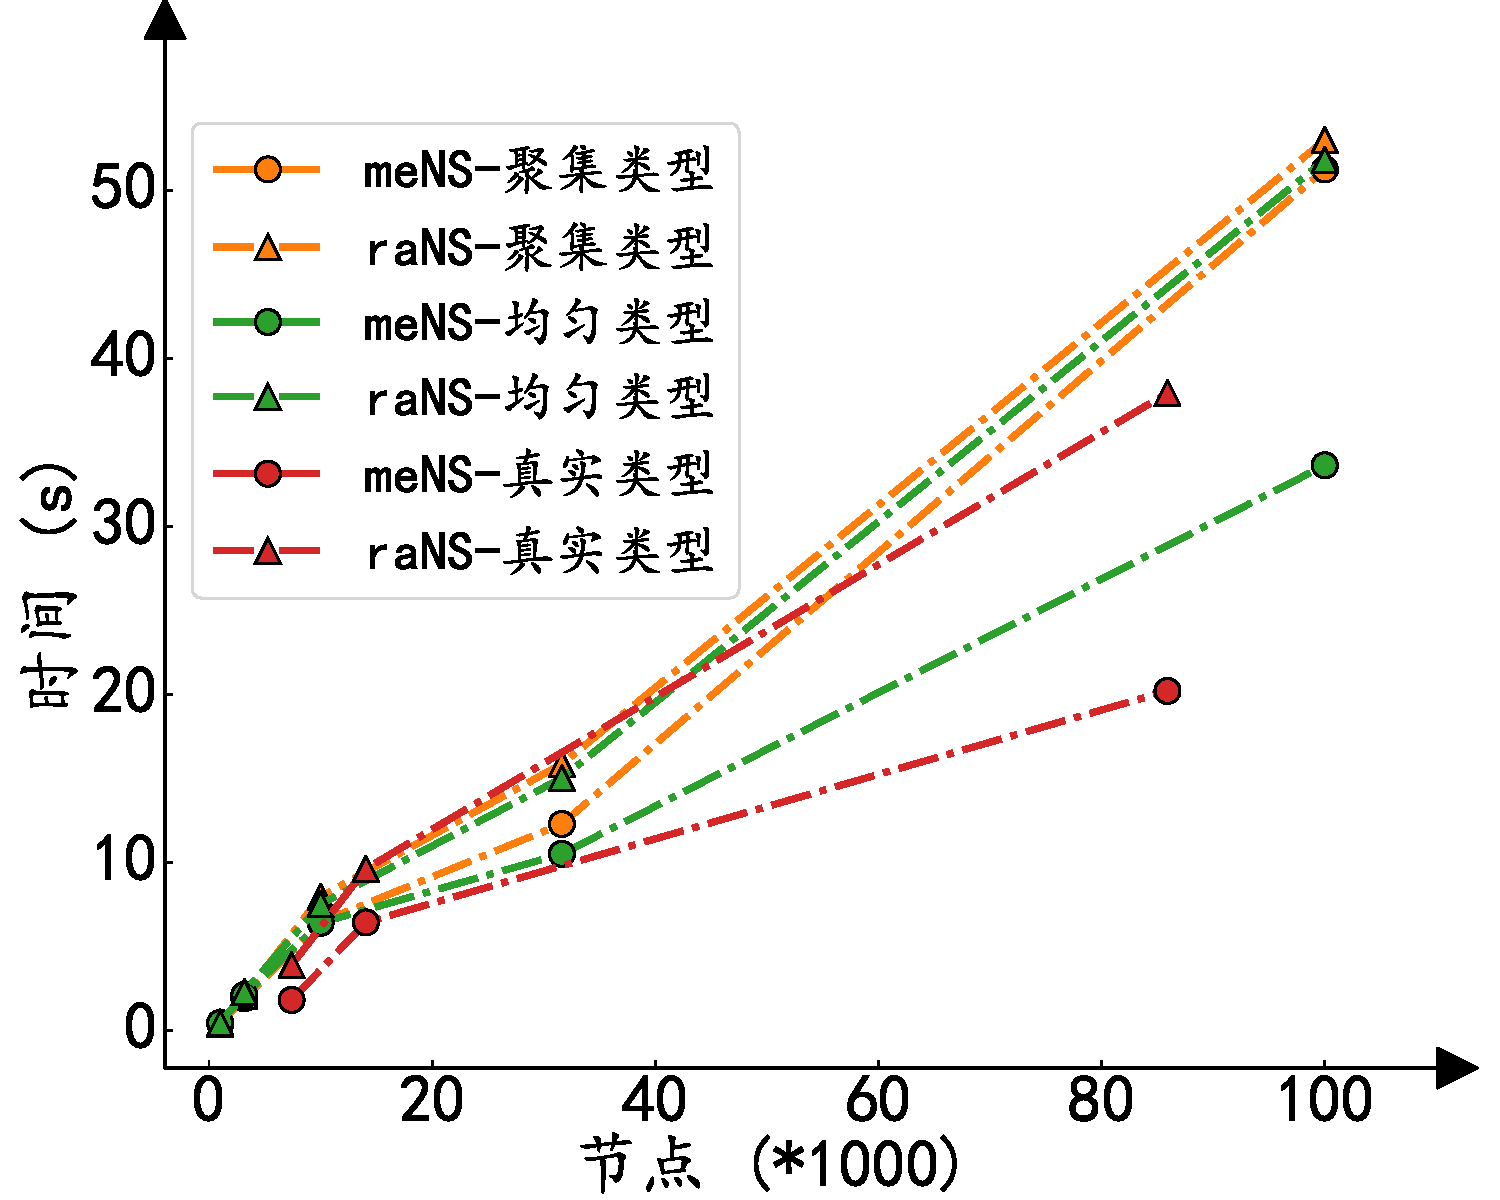
\includegraphics[width=.3\linewidth]{meNS时间对比.pdf}}
    \caption[各算法在均匀分布型用例$E10K$生成的邻域结构]{各算法在均匀分布型用例$E10K$生成的邻域结构}
    \label{fig:各算法在均匀分布型用例E10K生成的邻域结构}
\end{figure}
\begin{figure}[!h]
    \subfloat[meNS]{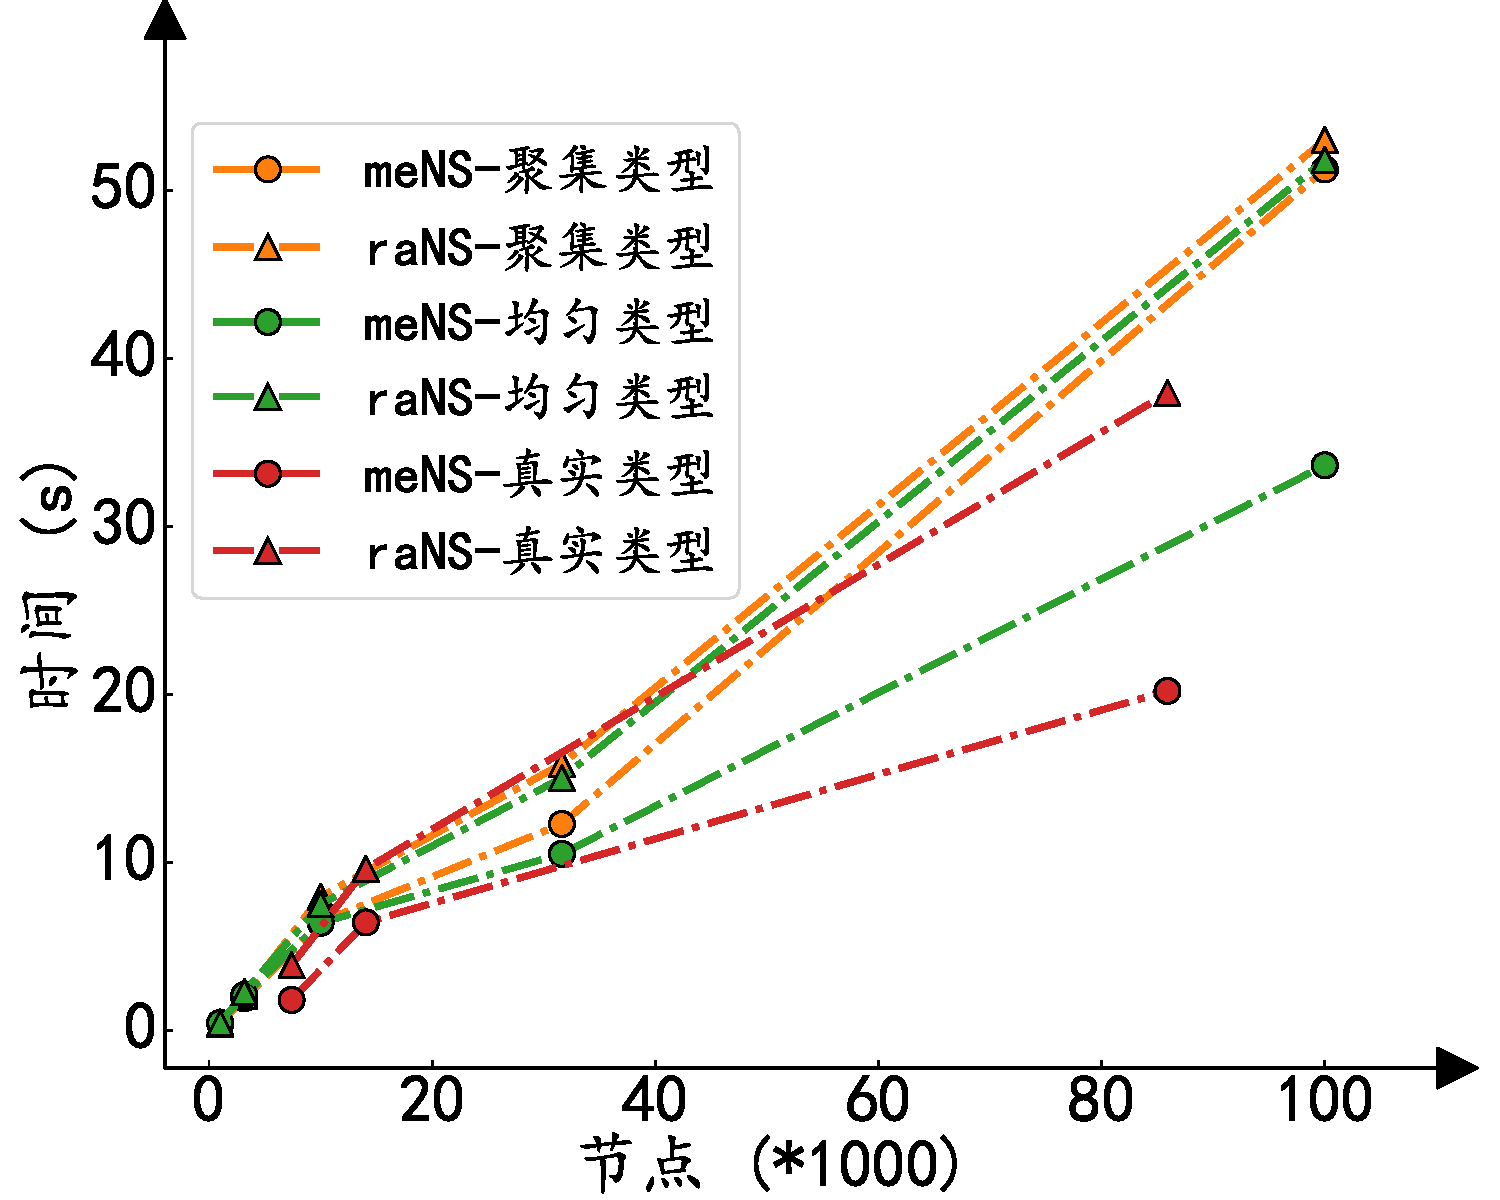
\includegraphics[width=.3\linewidth]{meNS时间对比.pdf}}
    \subfloat[K-NN]{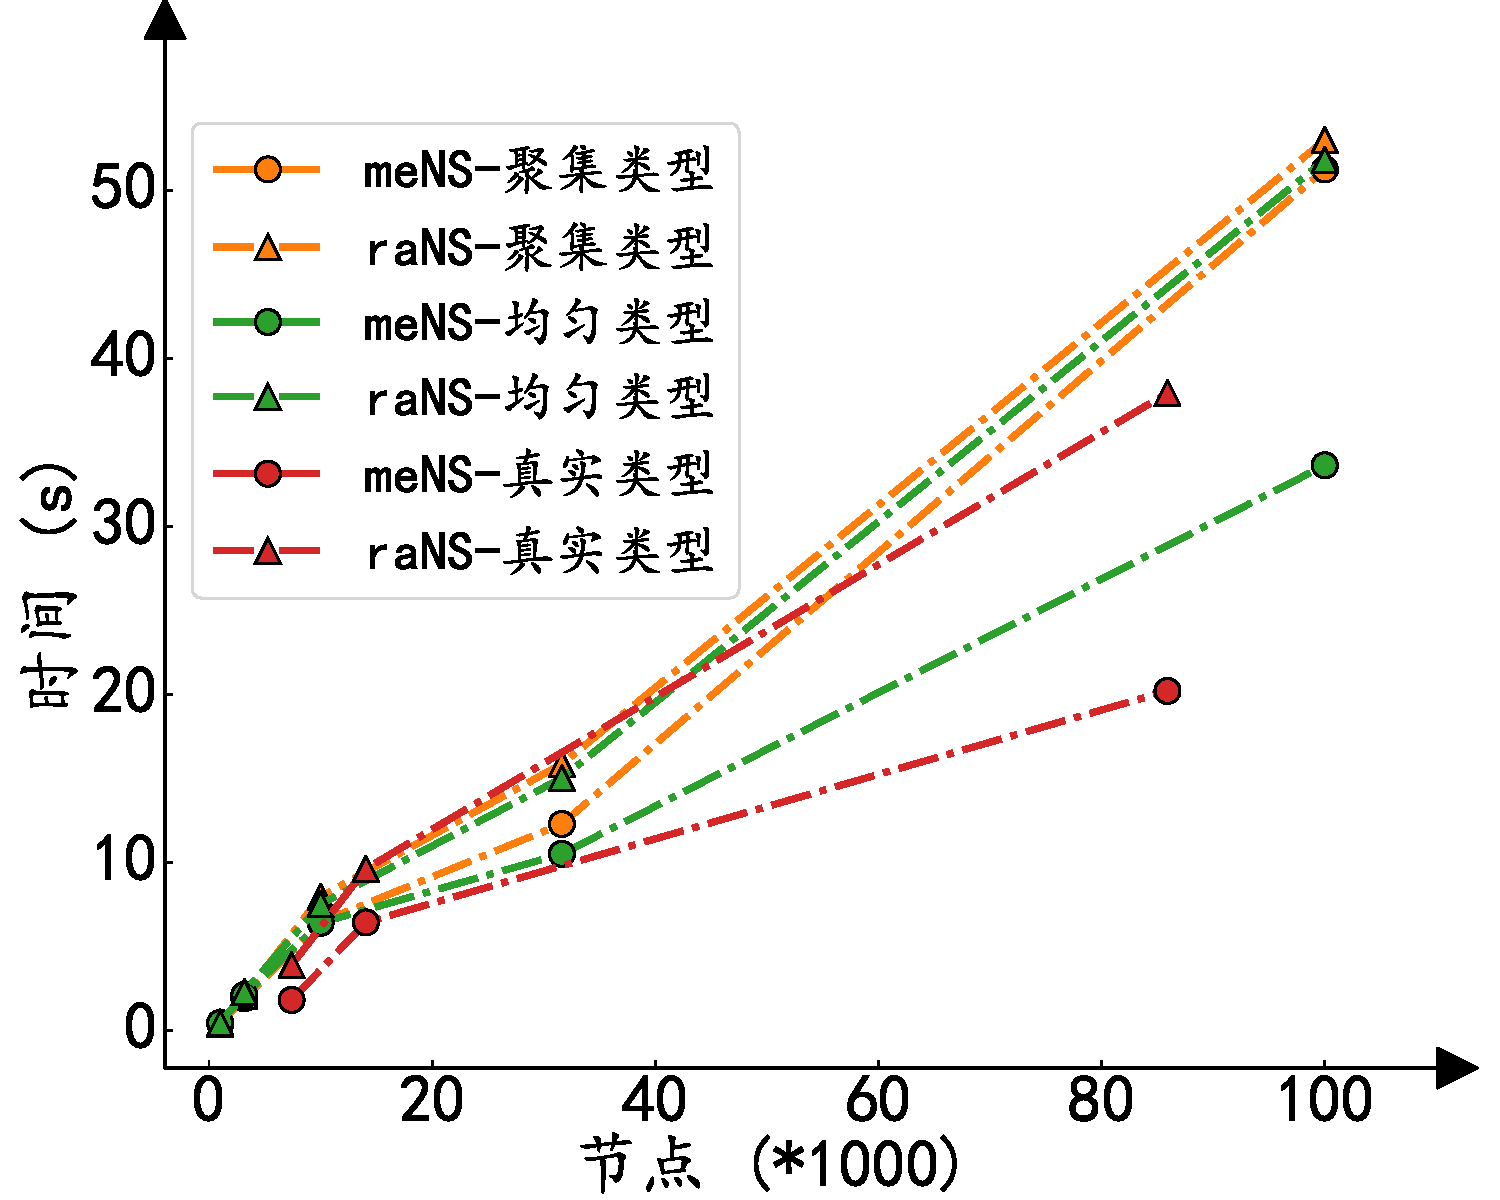
\includegraphics[width=.3\linewidth]{meNS时间对比.pdf}} \\
    \subfloat[$\alpha$-nearest ]{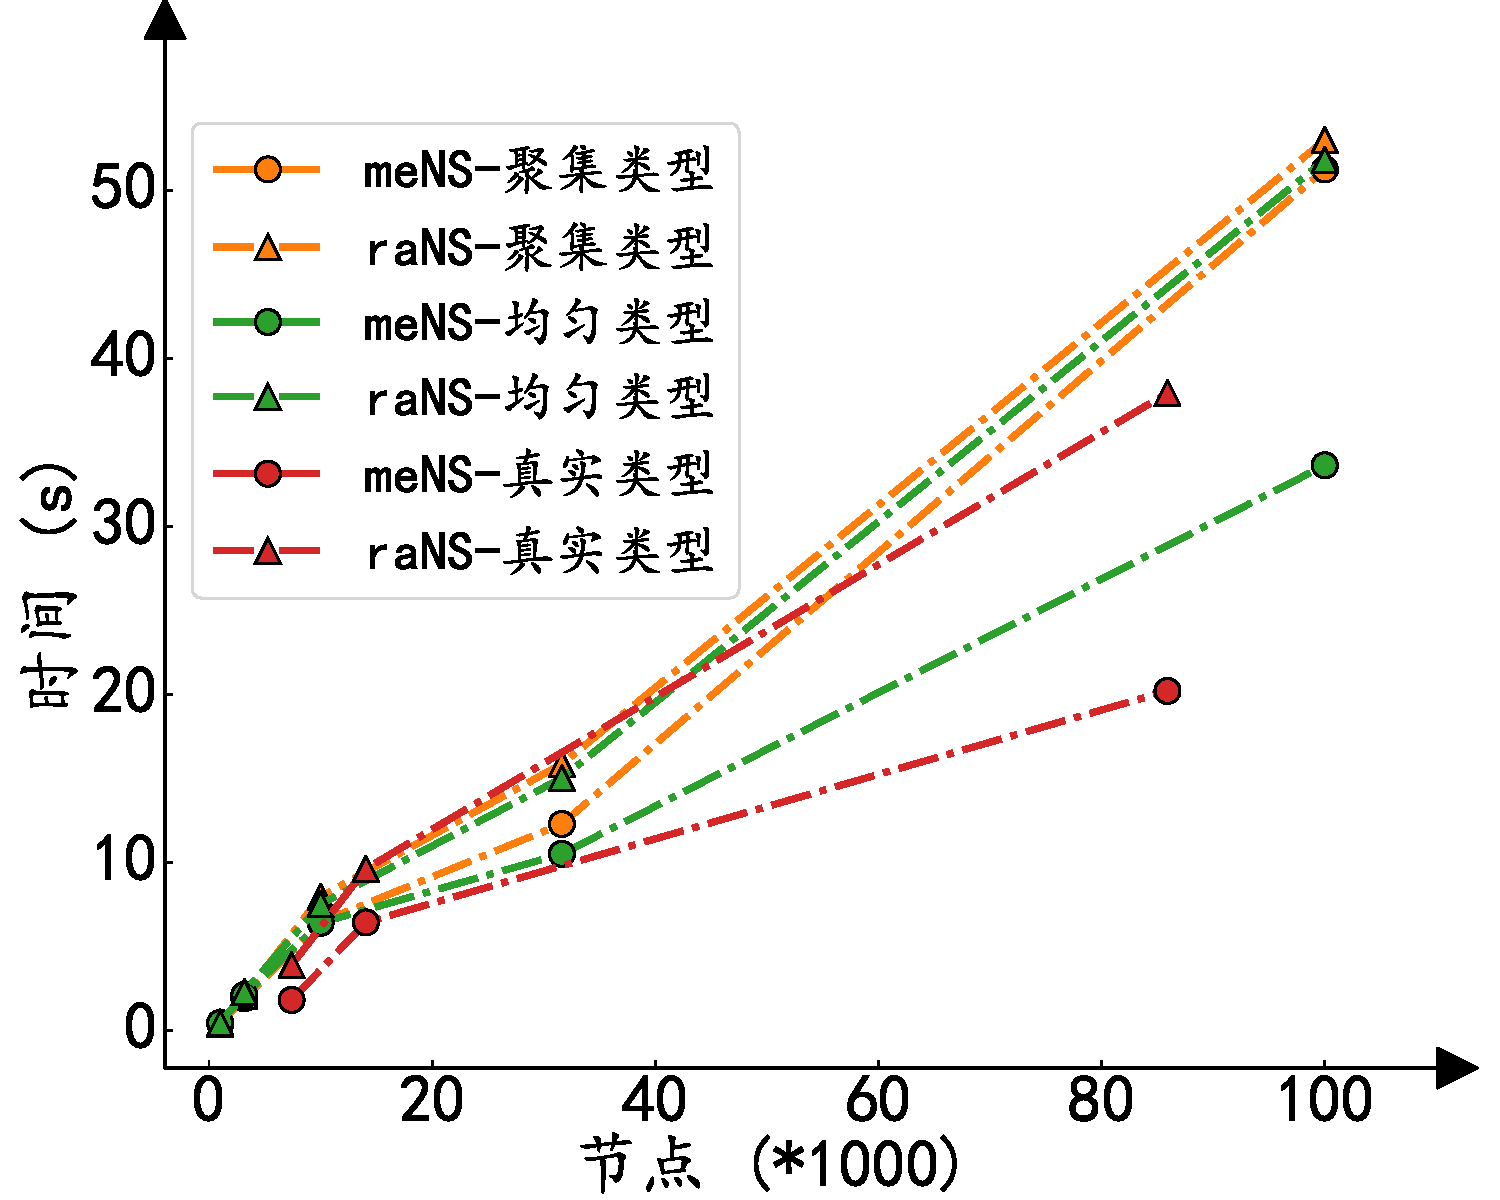
\includegraphics[width=.3\linewidth]{meNS时间对比.pdf}}
    \subfloat[Delaunay]{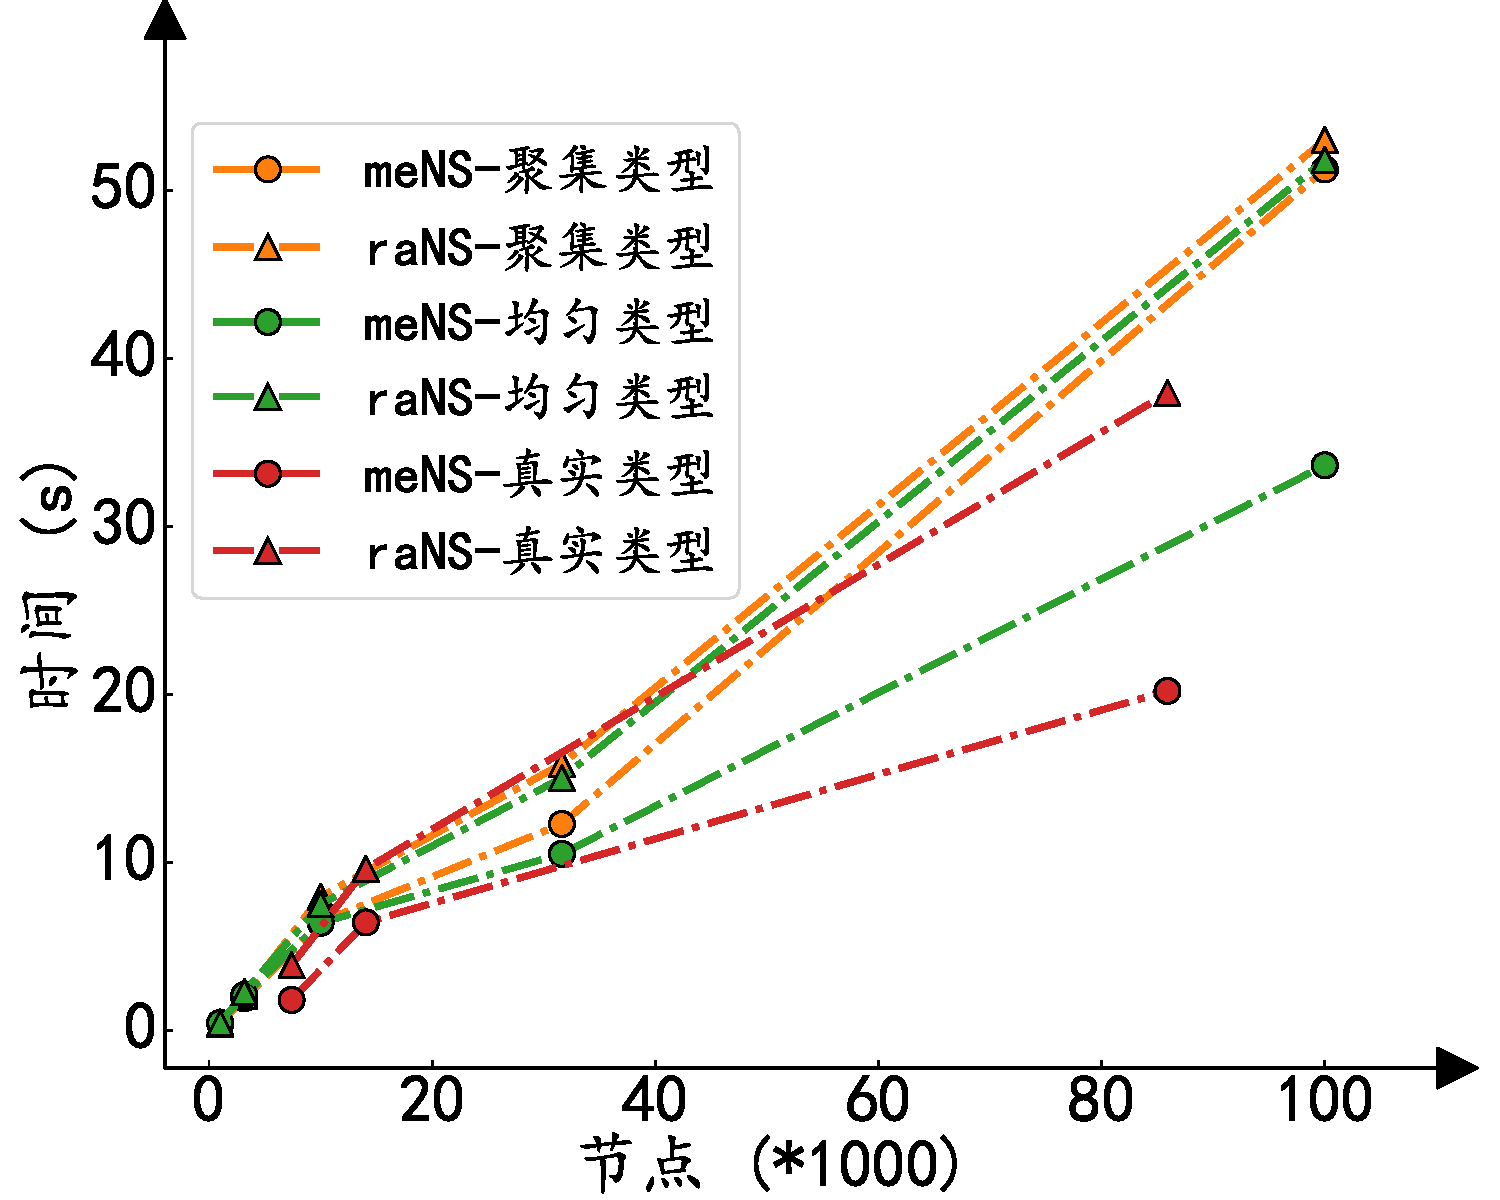
\includegraphics[width=.3\linewidth]{meNS时间对比.pdf}}
    \caption[各算法在印刷电路板测试用例$pla7397$生成的邻域结构]{各算法在印刷电路板测试用例$pla7397$生成的邻域结构}
    \label{fig:各算法在印刷电路板测试用例pla7397生成的邻域结构}
\end{figure}
\begin{figure}[!h]
    \subfloat[meNS]{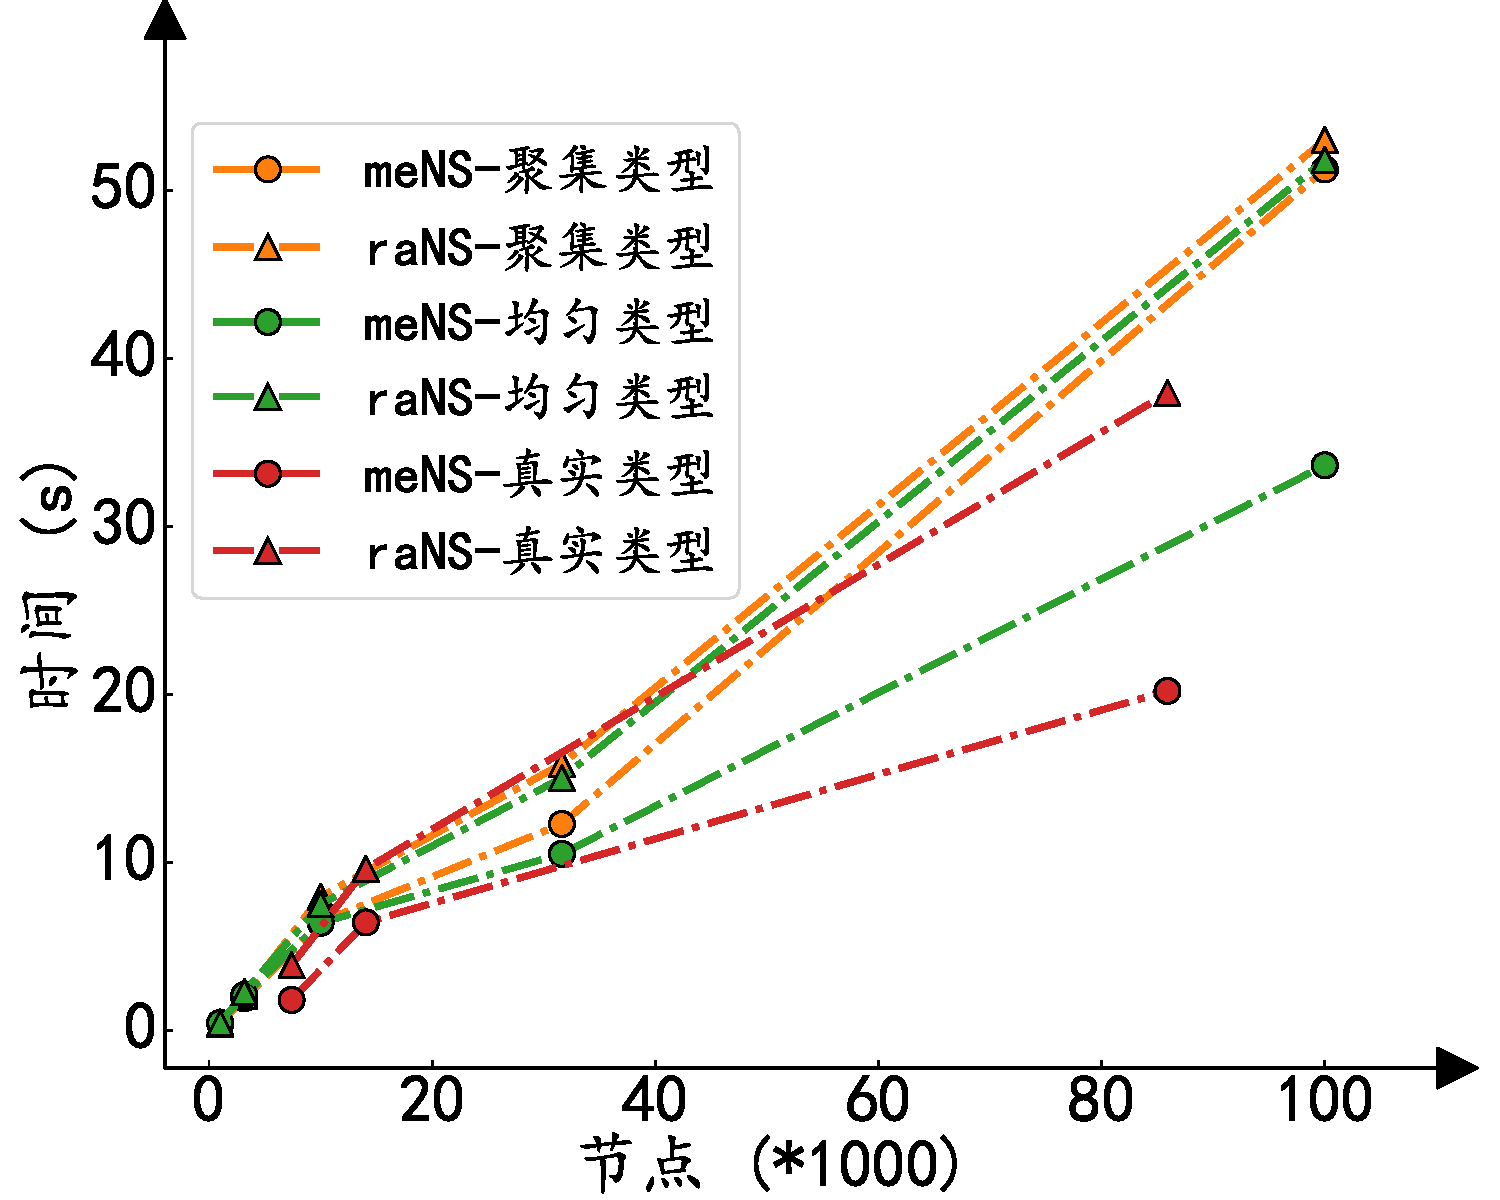
\includegraphics[width=.3\linewidth]{meNS时间对比.pdf}}
    \subfloat[K-NN]{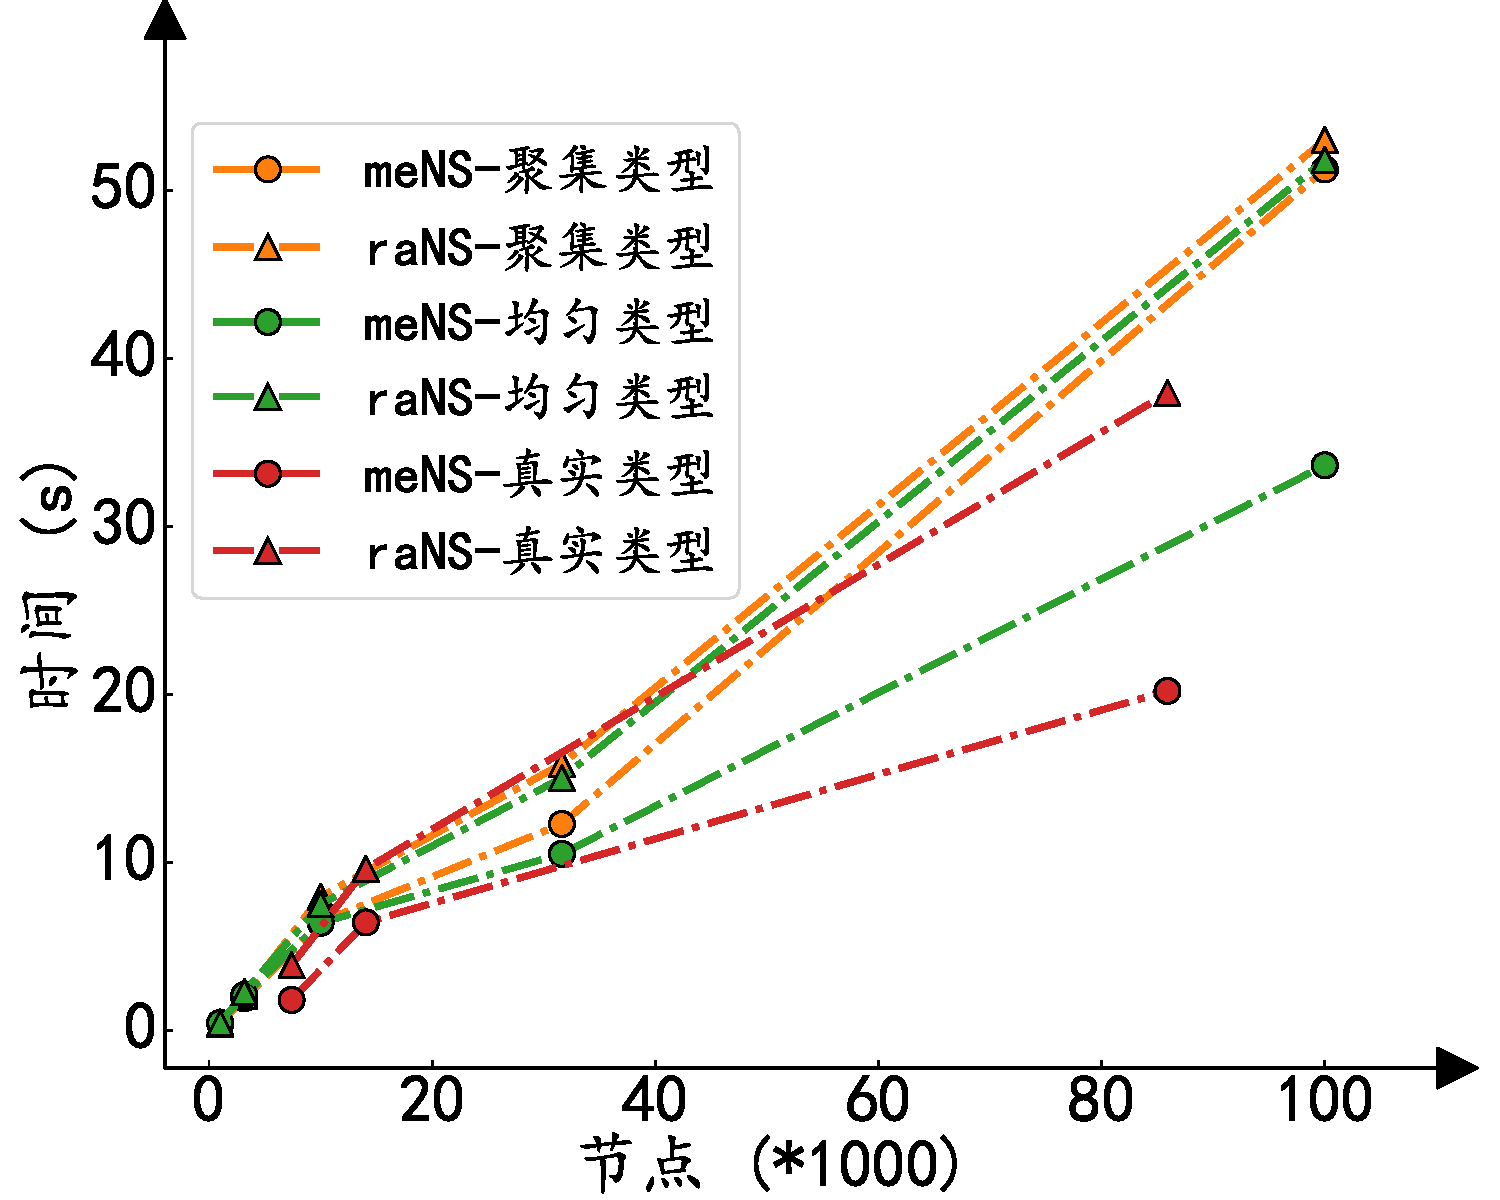
\includegraphics[width=.3\linewidth]{meNS时间对比.pdf}} \\
    \subfloat[$\alpha$-nearest ]{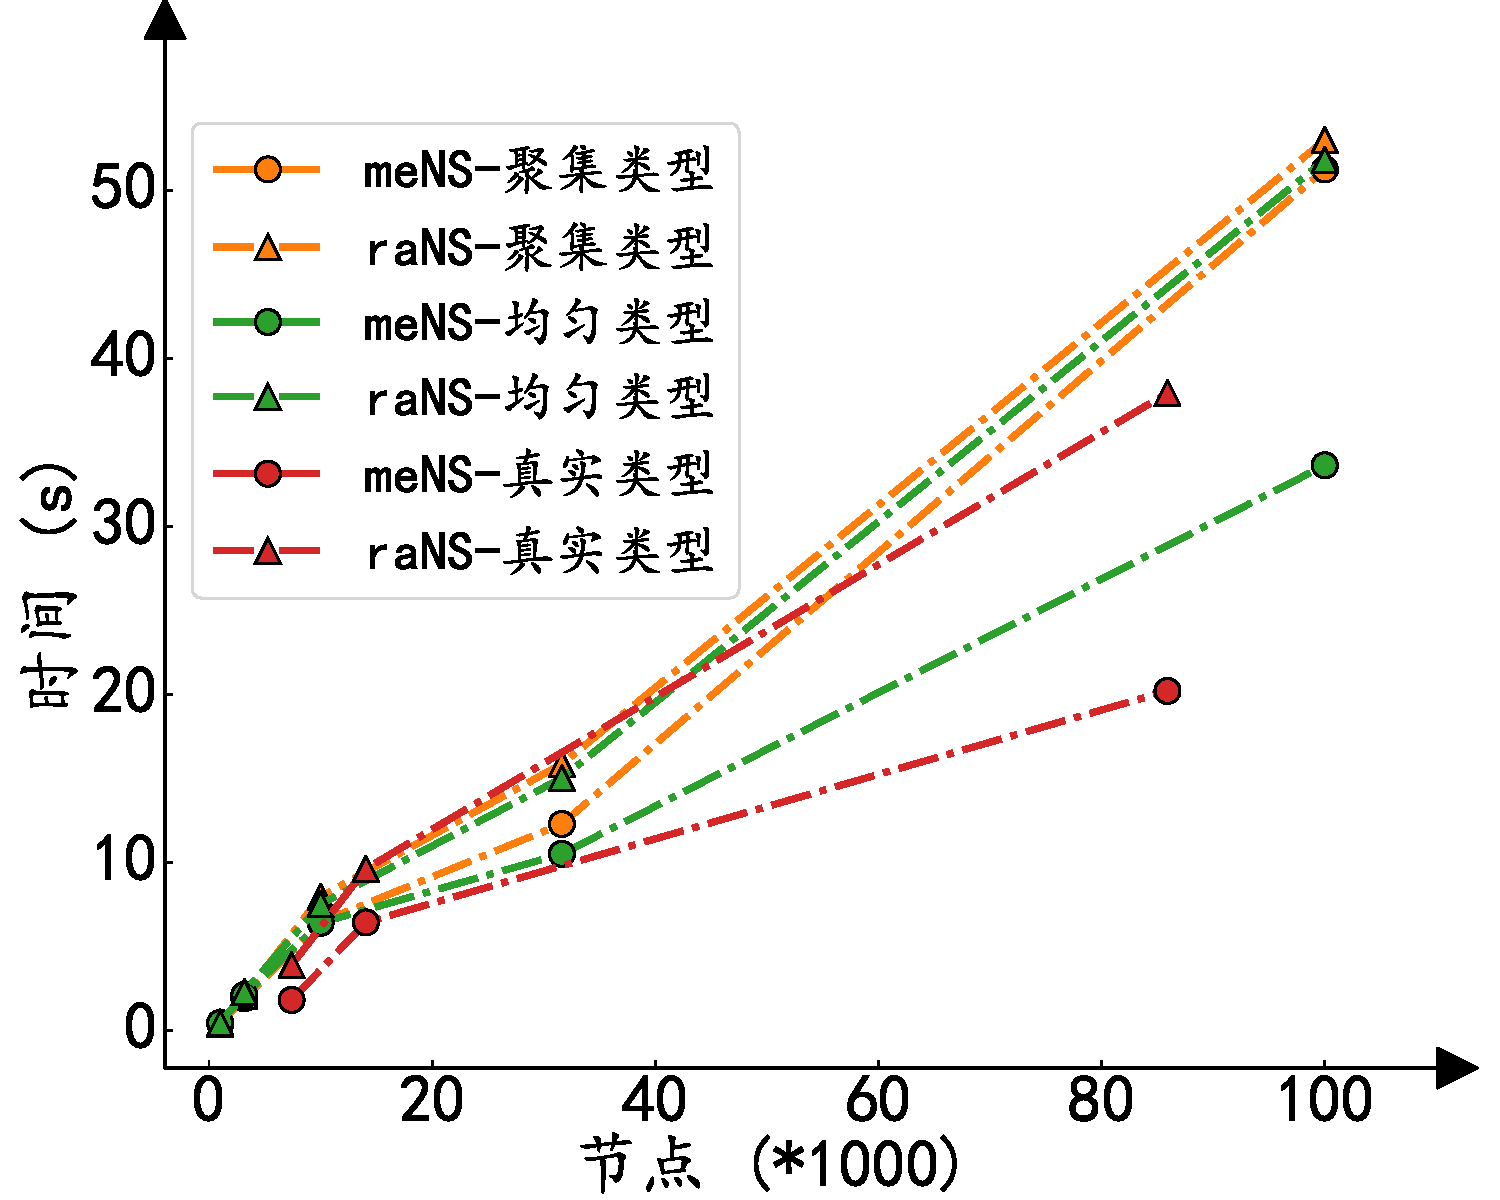
\includegraphics[width=.3\linewidth]{meNS时间对比.pdf}}
    \subfloat[Delaunay]{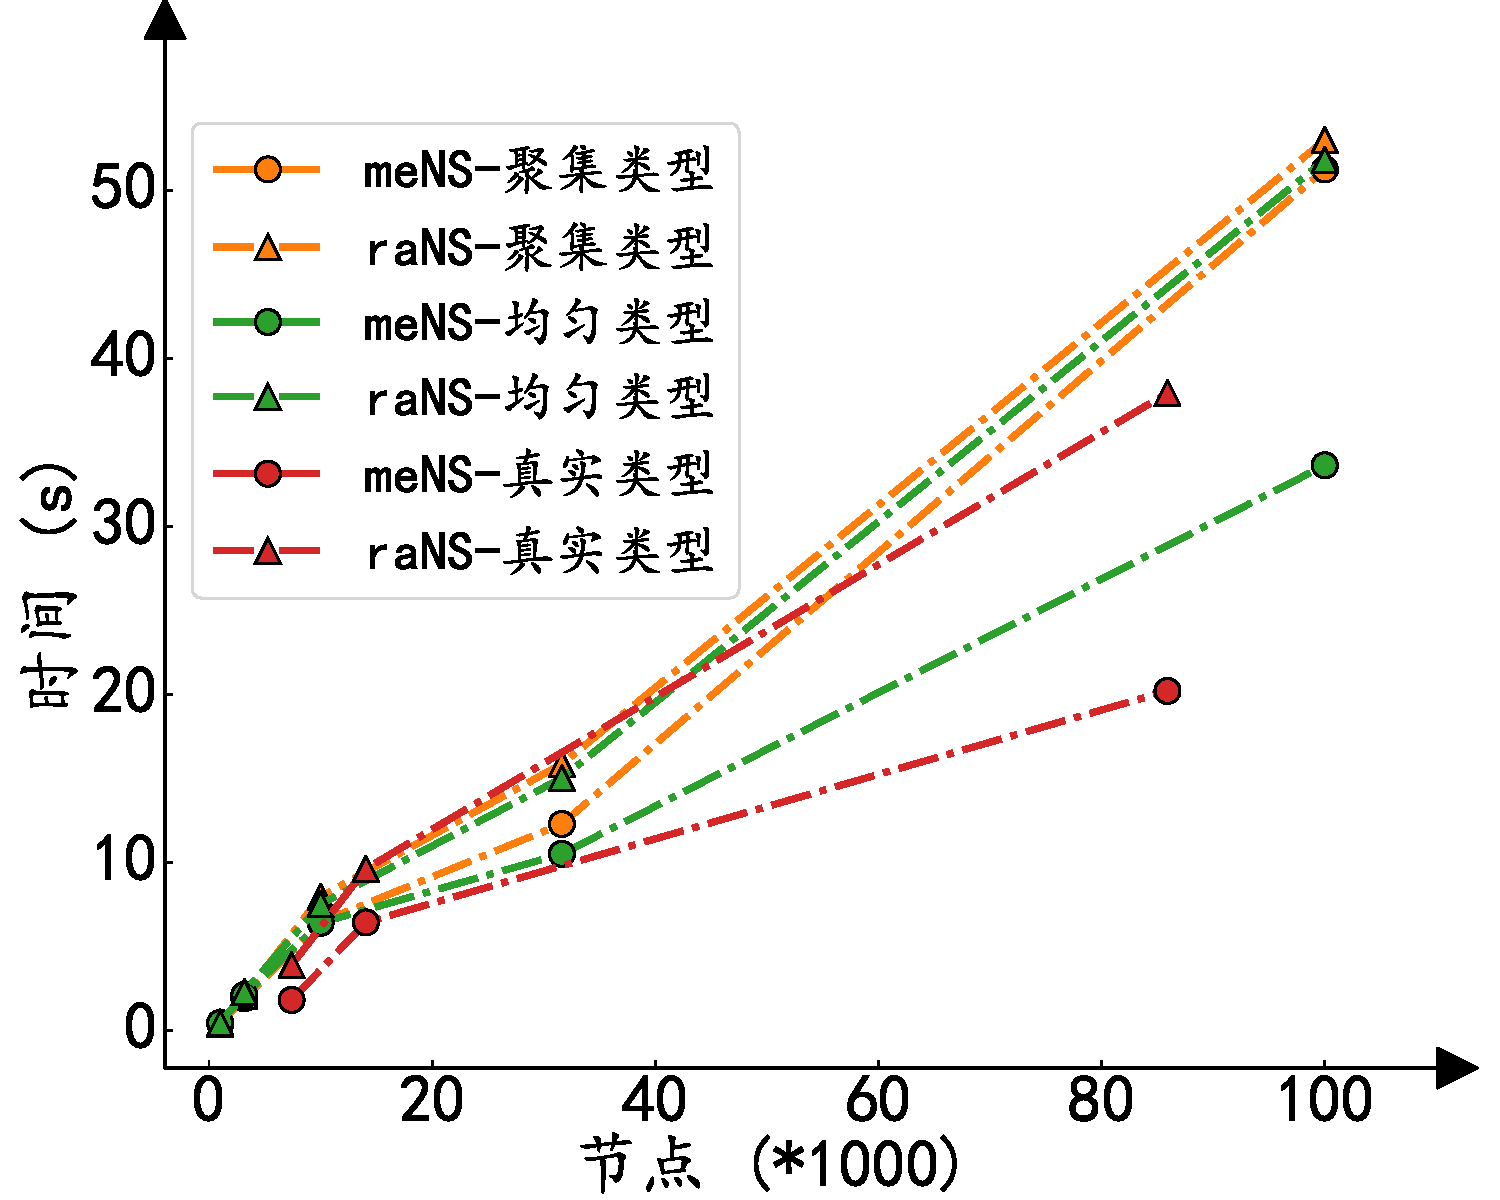
\includegraphics[width=.3\linewidth]{meNS时间对比.pdf}}
    \caption[各算法在真实地理位置测试用例$brd14051$生成的邻域结构]{各算法在真实地理位置测试用例$brd14051$生成的邻域结构}
    \label{fig:各算法在真实地理位置测试用例brd14051生成的邻域结构}
\end{figure}
\par
从NS Degree指标数据可以知道,虽然meNS生成的邻域结构在修剪后要比其他算法生成的邻域结构在修剪后更加的稀疏,但是这并不意味着meNS的质量会比其他算法的邻域结构的质量要差。从\autoref{tab:各算法表现}~中的最优边遗失率Missing指标数据和LKH最终解的距离趋近度LKH Gap指标数据上可以分析出,在大多数测试用例上,meNS生成的邻域结构在修剪后,其Missing指标值与其他算法生成的邻域结构在修剪后的Missing指标值相差不大,甚至更低,并且在LKH Gap指标数据上,meNS也比其他算法在大多数测试用例上要好。这就意味着,meNS生成算法不仅能够在合理的时间内产生比其他算法更加稀疏的邻域结构,而且在大多数测试用例上,其质量也不比其他算法的邻域结构的质量要低,甚至更好。这从多个方面验证了meNS生成算法的有效性。

\section{本章小结}
\label{sec:NS_Method:本章小结}
本章提出了一种利用最小生成树和欧拉回路来生成邻域结构(meNS)的方法。该算法能够将次梯度优化中产生的未被利用的中间产物1MST,以欧拉回路回路为中间桥梁,构造初始Tour并优化,最后使用这些被优化后的Tour来生成邻域结构。经过实验数据的比较与分析,可以知道meNS生成算法不仅能够在合理的时间内生成比其他算法更加稀疏的邻域结构,而且这些邻域结构能够包含最优Tour中的边,不少于其他算法生成的邻域结构,这意味着meNS生成算法生成的邻域结构更加稀疏的同时,其质量也不比其他算法生成的邻域结构差。
